% PREAMBLE
\documentclass[11pt, a4paper]{report}
\usepackage[utf8]{inputenc}
\usepackage{amsmath, amssymb, amsfonts}
\usepackage{graphicx, geometry, hyperref, fancyhdr, titlesec, xcolor}
\usepackage{tikz}
\usetikzlibrary{decorations.pathmorphing, decorations.markings, arrows.meta, calc}
\geometry{margin=0.8in}

\hypersetup{
colorlinks=true,
linkcolor=blue,
urlcolor=blue,
citecolor=blue
}

\titleformat{\chapter}[display]{\normalfont\Large\bfseries}{\chaptertitlename\ \thechapter}{1em}{}
\titlespacing*{\chapter}{0pt}{5pt}{15pt}
\titleformat{\section}{\normalfont\Large\bfseries\itshape}{\thesection}{1em}{}
\titleformat{\subsection}{\normalfont\large\itshape}{\thesubsection}{1em}{}
\titleformat{\subsubsection}{\normalfont\normalsize\itshape}{\thesubsubsection}{1em}{}

\pagestyle{fancy}
\fancyhf{}
\fancyhead[L]{\nouppercase{\leftmark}}
\fancyfoot[C]{\thepage}
\renewcommand{\headrulewidth}{1pt}
\renewcommand{\footrulewidth}{1pt}

\begin{document}

\begin{titlepage}
    \begin{center}
        \vspace*{28.45pt}
            
        \Huge
        \textbf{Foundations of General Relativity: From Flat Spacetime to the Schwarzschild Solution}
            
        \vspace{14.23pt}
        \LARGE
        A Mathematical and Geometric Approach to Gravitation
            
        \vspace{42.68pt}
            
        \textbf{Abdelrahman Mohamed Anwar}
            
        \vfill
            
        \Large
        A thesis presented for the degree of\\
        Bachelor of Science
            
        \vspace{22.76pt}
            
        \Large
        Department of Physics\\
        Ain Shams University\\
        2026
            
    \end{center}
\end{titlepage}

\newpage
\thispagestyle{empty}

\begin{abstract}
This thesis provides a comprehensive, mathematically rigorous review of General Relativity, tracing the theoretical development from the postulates of flat spacetime to the exact solutions of Einstein's field equations. We begin by formalizing Special Relativity using four-vector formalism and analyzing causality through the light cone structure. The mathematical framework of pseudo-Riemannian manifolds, tensor calculus, and differential forms is then systematically developed to describe curved spacetime. Utilizing the Einstein Equivalence Principle and minimal coupling, we derive the geodesic equation and Einstein's field equations, including discussions on the Newtonian limit, the Hilbert action, and the various energy conditions. Finally, we rigorously derive the Schwarzschild solution for a static, spherically symmetric vacuum. The causal structure of the Schwarzschild black hole is examined using Eddington-Finkelstein coordinates, and the classical experimental tests of General Relativity—specifically the precession of the perihelion and gravitational redshift—are analyzed. This work serves as a foundational synthesis of the geometric approach to gravitation, establishing the necessary groundwork for advanced studies in theoretical cosmology and high-energy physics.
\end{abstract}

\newpage
\tableofcontents
\newpage

\newcommand{\eqn}[1]{\hyperref[#1]{\eqref{#1}}}

\chapter{Special Relativity and Flat Spacetime}

\section{Prelude}

\subsection*{Core Concept of General Relativity (GR)}
General relativity posits that gravity is not a traditional force, but a manifestation of spacetime curvature.

\subsection*{Newtonian Gravity: A Review}
\textbf{Force-Based Formulation:}
\begin{equation}\label{eq:newton-force}
F = - \frac{GMm}{r^2} \hat{e}_r
\end{equation}
\begin{equation}\label{eq:newton-second}
F = ma
\end{equation}

\textbf{Potential-Based Formulation:}
Using \eqn{eq:newton-force} and \eqn{eq:newton-second}:
\begin{equation}
a = -\frac{GM}{r^2} \hat{e_r}
\end{equation}
Gravitational flux for enclosed mass $M_{\text{enclosed}} = \int_v \rho dV$:


$$Flux  = \oint_s a \cdot dA = - 4 \pi G M_{\text{enclosed}}$$

$$\oint_s a \cdot dA = - 4 \pi G \int_v \rho dV$$


By the divergence theorem and $a = - \nabla \Phi$, Poisson's equation relates potential $\Phi$ to mass density $\rho$:
\begin{equation}\label{eq:poisson}
\nabla^2 \Phi = 4\pi G \rho
\end{equation}
\begin{equation}\label{eq:potential-accel}
a = -\nabla \Phi
\end{equation}

\subsection*{Generic Proof To Get Poisson's Equation}
\begin{equation}\label{eq:acc-dm}
da = - G \frac{dm}{|r - r'|^2} \hat{e}*{r-r'}
\end{equation}
\begin{equation}\label{eq:dm_rho}
dM = \rho(\mathbf{r}') dV'
\end{equation}
\begin{equation}\label{eq:flux}
\Phi = \oint_S \mathbf{a} \cdot d\mathbf{A}
\end{equation}
Integrating acceleration over the source volume:
\begin{align*}
a(r) &= \int*{V_{\text{source}}} -G \frac{\rho(\mathbf{r}')}{|\mathbf{r}-\mathbf{r}'|^2} \hat{\mathbf{e}}*{(\mathbf{r}-\mathbf{r}')} dV'
\end{align*}
Evaluating the flux $\Phi$ given the surface integral is $4\pi$ when the source is inside:
\begin{equation}\label{flux_mass}
\Phi = -4 \pi G \int*{V_{\text{source}}}\rho(\mathbf{r}') dV'
\end{equation}
Yielding:
\begin{align*}
\int_V (\nabla \cdot \mathbf{a}) dV &= -4 \pi G \int_{V_{\text{source}}}\rho(\mathbf{r}') dV' \\
\nabla \cdot \mathbf{a} &= -4 \pi G \rho(\mathbf{r'}) \\
\nabla^2 \Phi &= 4 \pi G \rho(\mathbf{r'})
\end{align*}

\subsection*{General Relativity: A Preview}
Einstein's equation governs how energy-momentum curves spacetime:
\begin{equation}\label{eq:einstein}
R_{\mu\nu} - \frac{1}{2} R g_{\mu\nu} = 8\pi G T_{\mu\nu}
\end{equation}
Free particles traverse geodesics:
\begin{equation}\label{eq:geodesic}
\frac{d^2 x^{\mu}}{d\lambda^2} + \Gamma^{\mu}_{\rho\sigma} \frac{dx^{\rho}}{d\lambda} \frac{dx^{\sigma}}{d\lambda} = 0
\end{equation}

\section{Space and Time, Separately and Together}
Special relativity replaces Newtonian absolute time with a unified four-dimensional spacetime.

\subsection*{Spacetime and Worldlines}
\textbf{Spacetime:} 4D set of events.
\textbf{Worldline:} 1D curve of a particle's trajectory.

\subsection*{Relativistic Spacetime: The Light Cone Structure}
Special relativity eliminates absolute simultaneity. The invariant structure is the \emph{light cone}, defining causality. No signal can travel faster than light.

\begin{center}
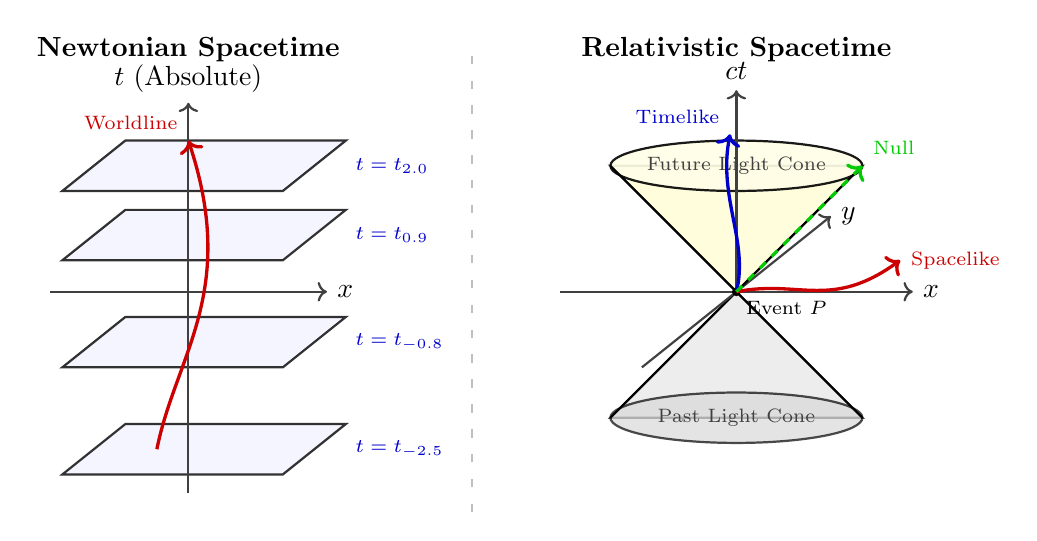
\begin{tikzpicture}[scale=0.8]
  % ----- Left: Newtonian Spacetime -----
  \begin{scope}[shift={(-4.5, 0)}]
    \node[above, font=\bfseries] at (0, 3.5) {Newtonian Spacetime};
    
    % Planes of absolute simultaneity
    \foreach \y in {-2.5, -0.8, 0.9, 2.0} {
      \draw[thick, fill=blue!5, opacity=0.8] (-2, \y-0.4) -- (1.5, \y-0.4) -- (2.5, \y+0.4) -- (-1, \y+0.4) -- cycle;
      \node[right, blue!80!black, font=\scriptsize] at (2.5, \y) {$t = t_{\y}$};
    }
    
    % Axes
    \draw[->, thick, darkgray] (0,-3.2) -- (0, 3.0) node[above, text=black] {$t$ (Absolute)};
    \draw[->, thick, darkgray] (-2.2,0) -- (2.2, 0) node[right, text=black] {$x$};
    
    % Particle worldline
    \draw[very thick, red!80!black, ->] (-0.5, -2.5) .. controls (-0.2, -1) and (0.8, 0) .. (0.0, 2.4) node[above left, font=\scriptsize] {Worldline};
  \end{scope}

  % ----- Divider -----
  \draw[thick, loosely dashed, gray!50] (0, -3.5) -- (0, 4);

  % ----- Right: Relativistic Spacetime -----
  \begin{scope}[shift={(4.2, 0)}]
    \node[above, font=\bfseries] at (0, 3.5) {Relativistic Spacetime};
    
    % Past Light Cone
    \draw[thick, fill=gray!20, opacity=0.7] (-2,-2) -- (0,0) -- (2,-2) -- cycle;
    \draw[thick, fill=gray!30, opacity=0.7] (0,-2) ellipse (2 and 0.4);
    \draw[thick] (-2,-2) -- (0,0) -- (2,-2);
    
    % Axes (drawn behind future cone, over past cone)
    \draw[->, thick, darkgray] (-2.8,0) -- (2.8, 0) node[right, text=black] {$x$};
    \draw[->, thick, darkgray] (-1.5,-1.2) -- (1.5, 1.2) node[right, text=black] {$y$};
    
    % Future Light Cone
    \draw[thick, fill=yellow!20, opacity=0.7] (-2,2) -- (0,0) -- (2,2) -- cycle;
    \draw[thick, fill=yellow!10, opacity=0.9] (0,2) ellipse (2 and 0.4);
    \draw[thick] (-2,2) -- (0,0) -- (2,2);
    \draw[->, thick, darkgray] (0,0) -- (0, 3.2) node[above, text=black] {$ct$};
    
    % Labels for regions
    \node[font=\scriptsize, darkgray] at (0, -2) {Past Light Cone};
    \node[font=\scriptsize, darkgray] at (0, 2) {Future Light Cone};

    % Origin Event
    \fill[black] (0,0) circle (2pt) node[below right, font=\scriptsize] {Event $P$};

    % Causal Structure Worldlines
    % Timelike
    \draw[very thick, blue!80!black, ->] (0,0) .. controls (0.2, 0.8) and (-0.3, 1.5) .. (-0.1, 2.5) node[above left, font=\scriptsize] {Timelike};
    % Spacelike
    \draw[very thick, red!80!black, ->] (0,0) .. controls (1, 0.2) and (1.5, -0.3) .. (2.6, 0.5) node[right, font=\scriptsize] {Spacelike};
    % Null (on the cone)
    \draw[very thick, green!80!black, dashed, ->] (0,0) -- (2, 2) node[above right, font=\scriptsize] {Null};
  \end{scope}

\end{tikzpicture}
\end{center}

\subsection*{The Invariant Spacetime Interval}
The interval remains invariant for all inertial observers:

$$(\Delta s)^2 = - (c \Delta t)^2 + (\Delta x)^2 + (\Delta y)^2 + (\Delta z)^2 = - (c \Delta t')^2 + (\Delta x')^2 + (\Delta y')^2 + (\Delta z')^2$$

Defining coordinates $x^\mu = (t, x, y, z)$ with $c=1$, the flat spacetime (Minkowski) metric is:
\begin{equation}\label{eq:minkowski-metric}
\eta_{\mu\nu} = \text{diag}(-1, 1, 1, 1)
\end{equation}

\subsection*{Causal Structure and Proper Time}
\begin{itemize}
\item \textbf{Timelike:} $(\Delta s)^2 < 0$
\item \textbf{Spacelike:} $(\Delta s)^2 > 0$
\item \textbf{Null:} $(\Delta s)^2 = 0$
\end{itemize}
Proper time for timelike separations:
\begin{equation}\label{eq:proper-time}
(\Delta \tau)^2 = -(\Delta s)^2 = -\eta_{\mu\nu} \Delta x^\mu \Delta x^\nu
\end{equation}

\subsection*{General Trajectories}
For any timelike trajectory $x^\mu(\lambda)$:

$$\Delta \tau = \int \sqrt{ -\eta_{\mu\nu} \frac{dx^\mu}{d\lambda} \frac{dx^\nu}{d\lambda} } d\lambda$$

\section{Lorentz Transformations}
\subsection*{Translations and Linear Transformations}
Translations:
\begin{equation}\label{eq:translation}
x^{\mu'} = \delta^{\mu'}*\mu (x^\mu + a^\mu)
\end{equation}
Linear Transformations (Rotations and Boosts):
\begin{equation}\label{eq:linear-transform}
x^{\mu'} = \Lambda^{\mu'}*\nu x^\nu
\end{equation}

\subsection*{Condition for Lorentz Transformation}
Invariance of $(\Delta s)^2$ requires:
\begin{equation}\label{eq:lorentz-condition}
\eta = \Lambda^T \eta \Lambda \quad \text{or} \quad \eta_{\rho\sigma} = \Lambda^{\mu'}*\rho \Lambda^{\nu'}*\sigma \eta_{\mu'\nu'}
\end{equation}
This defines the \textbf{Lorentz group O(3,1)}. The \textbf{Poincaré group} includes both Lorentz transformations and translations.

\subsection*{Explicit Transformation Matrices}
\textbf{Spatial Rotation} (e.g., $x-y$ plane):
\begin{equation}\label{eq:rotation-matrix}
{\Lambda^{\mu'}}_{\nu} =
\begin{pmatrix}
1 & 0 & 0 & 0 \\
0 & \cos\theta & \sin\theta & 0 \\
0 & -\sin\theta & \cos\theta & 0 \\
0 & 0 & 0 & 1
\end{pmatrix}
\end{equation}

\textbf{Boost} (along $x$-direction, rapidity $\phi$):
\begin{equation}\label{eq:boost-matrix}
{\Lambda^{\mu'}}_{\nu} =
\begin{pmatrix}
\cosh\phi & -\sinh\phi & 0 & 0 \\
-\sinh\phi & \cosh\phi & 0 & 0 \\
0 & 0 & 1 & 0 \\
0 & 0 & 0 & 1
\end{pmatrix}
\end{equation}
Setting $v = \tanh\phi$ and $\gamma = 1/\sqrt{1-v^2}$, this becomes:
\begin{align}
t' &= \gamma(t - vx) \label{eq:lorentz-tprime} \\
x' &= \gamma(x - vt) \label{eq:lorentz-xprime}
\end{align}

\section{Vectors}
Vectors reside in the \textbf{tangent space} $T_p$ at a given point $p$.

\begin{center}
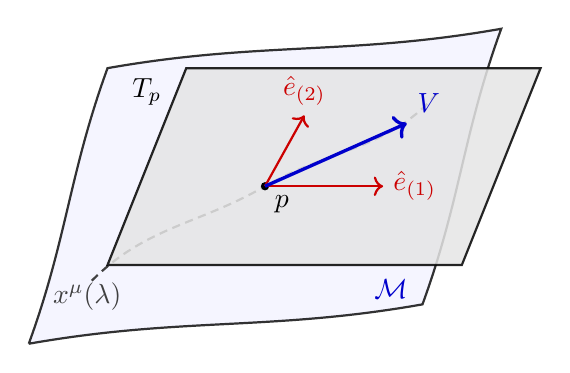
\begin{tikzpicture}[scale=1.0]
  % Define the center point p
  \coordinate (P) at (3, 2);

  % Draw the curved manifold (surface M)
  \draw[thick, fill=blue!5, opacity=0.8] 
    (0,0) to[out=10, in=190] (5,0.5) 
          to[out=70, in=250] (6,4) 
          to[out=190, in=10] (1,3.5) 
          to[out=250, in=70] (0,0);
  \node[blue!80!black] at (4.6, 0.7) {$\mathcal{M}$};

  % Draw a curve x^\mu(\lambda) on the manifold passing through p
  \draw[thick, densely dashed, darkgray] 
    (0.8, 0.8) to[out=45, in=210] (P) to[out=30, in=230] (5.2, 3.2);
  \node[darkgray, above left] at (1.3, 0.3) {$x^\mu(\lambda)$};

  % Draw the tangent plane T_p at point p
  \draw[thick, fill=gray!20, opacity=0.85] 
    (1, 1) -- (5.5, 1) -- (6.5, 3.5) -- (2, 3.5) -- cycle;
  \node at (1.5, 3.2) {$T_p$};

  % Mark the point p
  \fill[black] (P) circle (1.5pt) node[below right] {$p$};

  % Basis vectors e_(\mu) on the tangent plane
  \draw[->, thick, red!80!black] (P) -- ++(1.5, 0) node[right] {$\hat{e}_{(1)}$};
  \draw[->, thick, red!80!black] (P) -- ++(0.5, 0.9) node[above] {$\hat{e}_{(2)}$};

  % Tangent vector V^\mu = dx^\mu / d\lambda
  \draw[->, very thick, blue!80!black] (P) -- ++(1.8, 0.8) node[above right] {$V$};

\end{tikzpicture}
\end{center}

\subsection*{Basis and Transformation}
A vector $A = A^\mu \hat{e}_{(\mu)}$. The tangent vector to $x^\mu(\lambda)$ is $V^\mu = dx^\mu/d\lambda$.
Vector components transform via $\Lambda$:
\begin{equation}
V^{\mu'} = {\Lambda^{\mu'}}*\nu V^\nu
\end{equation}
Basis vectors transform inversely to keep the geometric vector invariant:
\begin{equation}
\hat{e}*{(\nu')} = {\Lambda^\mu}*{\nu'} \hat{e}*{(\mu)}
\end{equation}

\section{Dual Vectors (One-Forms)}
The \textbf{cotangent space} $T_p^*$ contains dual vectors $\omega$, linear maps from $T_p \to \mathbb{R}$.

\subsection*{Basis and Action}
Basis dual vectors satisfy $\hat{\theta}^{(\nu)}(\hat{e}_{(\mu)}) = \delta^\nu_\mu$. Expanding $\omega = \omega_\mu \hat{\theta}^{(\mu)}$:
\begin{equation}
\omega(V) = \omega_\mu V^\mu \in \mathbb{R}
\end{equation}

\subsection*{Transformation}
Dual vector components transform via the inverse matrix:
\begin{equation}
\omega_{\mu'} = {\Lambda^\nu}*{\mu'} \omega*\nu
\end{equation}

\subsection*{Gradient}
The gradient $d\phi = \partial_\mu \phi \hat{\theta}^{(\mu)}$ is a natural dual vector:
\begin{equation}
\frac{\partial\phi}{\partial x^{\mu'}} = {\Lambda^\nu}*{\mu'} \frac{\partial\phi}{\partial x^\nu}
\end{equation}
\begin{equation}
\partial*\mu\phi \frac{dx^\mu}{d\lambda} = \frac{d\phi}{d\lambda}
\end{equation}

\section{Tensors}
A $(k, l)$ tensor multilinearly maps $k$ dual vectors and $l$ vectors to $\mathbb{R}$.

\subsection*{Tensor Components}
Constructed via tensor products $\otimes$, components transform as:
\begin{equation}
{T^{\mu'_1 \dots \mu'*k}}*{\nu'_1 \dots \nu'*l} = {\Lambda^{\mu'*1}}*{\mu_1} \dots {\Lambda^{\nu_l}}*{\nu'*l} {T^{\mu_1 \dots \mu_k}}*{\nu_1 \dots \nu_l}
\end{equation}

\subsection*{Spacetime Tensors}
\begin{itemize}
\item \textbf{Metric $\eta_{\mu\nu}$:} $\eta(V, W) = \eta_{\mu\nu}V^\mu W^\nu$.
\item \textbf{Inverse Metric $\eta^{\mu\nu}$:} $\eta^{\mu\rho}\eta_{\rho\nu} = \delta^\mu_\nu$.
\item \textbf{Levi-Civita $\tilde{\epsilon}_{\mu\nu\rho\sigma}$:} $\pm 1$ for even/odd permutations.
\item \textbf{EM Field Tensor $F_{\mu\nu}$:}
\begin{equation}\label{eq:EM Field Tensor}
F_{\mu\nu} =
\begin{pmatrix}
0 & -E_1 & -E_2 & -E_3 \\
E_1 & 0 & B_3 & -B_2 \\
E_2 & -B_3 & 0 & B_1 \\
E_3 & B_2 & -B_1 & 0
\end{pmatrix}
= -F_{\nu\mu}
\end{equation}
\end{itemize}

\section{Manipulating Tensors}
\textbf{Contraction:} Summing one upper and one lower index (${S^{\mu\rho}}_\sigma = {T^{\mu\nu\rho}}_{\sigma\nu}$).
\textbf{Raising/Lowering:}
\begin{align}
{T^{\alpha\beta\mu}}*\delta &= \eta^{\mu\gamma} {T^{\alpha\beta}}*{\gamma\delta} \\
V_\mu &= \eta_{\mu\nu}V^\nu
\end{align}
\textbf{Trace:} Contraction of indices $X = {X^\lambda}_\lambda = \eta^{\mu\nu}Y_{\mu\nu}$.

\section{Maxwell's Equations}
\textbf{Inhomogeneous Equations:} Combine $\partial_i F^{0i} = J^0$ and $\partial_j F^{ji} - \partial_0 F^{0i} = J^i$:
\begin{equation}\label{eq:inhom-maxwell}
\partial_\mu F^{\nu\mu} = J^\nu
\end{equation}
\textbf{Homogeneous Equations:}
\begin{equation}\label{eq:hom-maxwell}
\partial_{[\mu} F_{\nu\lambda]} = 0 \quad \implies \quad \partial_\mu F_{\nu\lambda} + \partial_\nu F_{\lambda\mu} + \partial_\lambda F_{\mu\nu} = 0
\end{equation}
Manifest covariance ensures frame-independent validity.

\section{Energy and Momentum}
\subsection*{Four-Velocity and Four-Momentum}
\begin{equation}
U^\mu = \frac{dx^\mu}{d\tau}, \quad \eta_{\mu\nu}U^\mu U^\nu = -1
\end{equation}
\begin{equation}
p^\mu = mU^\mu, \quad p_\mu p^\mu = -m^2 \implies E = \sqrt{m^2 + p^2}
\end{equation}

\subsection*{Four-Force}
\begin{equation}
f^\mu = \frac{dp^\mu}{d\tau} = q {F^\mu}_\lambda U^\lambda
\end{equation}

\subsection*{Energy-Momentum Tensor $T^{\mu\nu}$}
$T^{\mu\nu}$ measures four-momentum flux.
\textbf{Dust:} $N^\mu = nU^\mu$ and $T^{\mu\nu}_{\text{dust}} = \rho U^\mu U^\nu$. Under arbitrary boost:
\begin{equation}
N^{\mu'} = n \gamma (1, -v_x, -v_y, -v_z)^T
\end{equation}
\begin{equation}
T^{\mu'\nu'} = \rho \gamma^2
\begin{pmatrix}
1 & -v_x & -v_y & -v_z \\
-v_x & v_x^2 & v_x v_y & v_x v_z \\
-v_y & v_y v_x & v_y^2 & v_y v_z \\
-v_z & v_z v_x & v_z v_y & v_z^2
\end{pmatrix}
\end{equation}

\textbf{Perfect Fluid:}
\begin{equation}
T^{\mu\nu} = (\rho+p)U^\mu U^\nu + p\eta^{\mu\nu}
\end{equation}
Under arbitrary boost:
\begin{equation}
T^{\mu'\nu'} =
\begin{pmatrix}
\gamma^2(\rho + p) - p & -\gamma^2 v_x (\rho + p) & -\gamma^2 v_y (\rho + p) & -\gamma^2 v_z (\rho + p) \\
-\gamma^2 v_x (\rho + p) & \gamma^2 v_x^2 (\rho + p) + p & \gamma^2 v_x v_y (\rho + p) & \gamma^2 v_x v_z (\rho + p) \\
-\gamma^2 v_y (\rho + p) & \gamma^2 v_y v_x (\rho + p) & \gamma^2 v_y^2 (\rho + p) + p & \gamma^2 v_y v_z (\rho + p) \\
-\gamma^2 v_z (\rho + p) & \gamma^2 v_z v_x (\rho + p) & \gamma^2 v_z v_y (\rho + p) & \gamma^2 v_z^2 (\rho + p) + p
\end{pmatrix}
\end{equation}

\subsection*{Conservation Law}
\begin{equation}\label{eq:cons-T}
\partial_\mu T^{\mu\nu} = \partial_\mu (\rho + p) U^\mu U^\nu + (\rho + p) U^\mu \partial_\mu U^\nu + (\rho + p) U^\nu \partial_\mu U^\mu + \partial^\nu p = 0
\end{equation}
Contracting with $U_\nu$ yields energy conservation (continuity eq: $\partial_t \rho + \nabla \cdot (\rho \mathbf{v}) = 0$). Projecting orthogonally to $U^\mu$ yields momentum conservation (Euler eq: $\rho[\partial_t \mathbf{v} + (\mathbf{v}\cdot\nabla)\mathbf{v}] = -\nabla p$).

\section{Classical Field Theory}
\subsection*{Euler-Lagrange Equations}
From $S = \int \mathcal{L}(\Phi^i, \partial_\mu\Phi^i) d^4x$:
\begin{equation}
\frac{\partial\mathcal{L}}{\partial\Phi^i} - \partial_\mu\left(\frac{\partial\mathcal{L}}{\partial(\partial_\mu\Phi^i)}\right) = 0
\end{equation}

\textbf{Scalar Field:} $\mathcal{L} = -\frac{1}{2}\eta^{\mu\nu}(\partial_\mu\phi)(\partial_\nu\phi) - V(\phi)$ yields Klein-Gordon:
\begin{equation}
\Box\phi + m^2\phi = 0
\end{equation}

\textbf{Electromagnetism:} $\mathcal{L} = -\frac{1}{4}F_{\mu\nu}F^{\mu\nu} + A_\mu J^\mu$ yields $\partial_\mu F^{\nu\mu} = J^\nu$.

\subsection*{Derived Energy-Momentum Tensors}
\begin{equation}
T^{\mu\nu}*{\text{scalar}} = (\partial^\mu\phi)(\partial^\nu\phi) - \eta^{\mu\nu}\left[\frac{1}{2}(\partial*\lambda\phi)(\partial^\lambda\phi) + V(\phi)\right]
\end{equation}
\begin{equation}
T^{\mu\nu}*{\text{EM}} = {F^{\mu\lambda}}{F^\nu}*\lambda - \frac{1}{4}\eta^{\mu\nu} F^{\lambda\sigma}F_{\lambda\sigma}
\end{equation}


\chapter{Manifolds}

\section{Gravity as Geometry}
Gravity is a manifestation of spacetime geometry, founded on the \textbf{Principle of Equivalence}.

\subsection*{The Weak Equivalence Principle (WEP)}
WEP asserts inertial mass ($m_i$) equals gravitational mass ($m_g$).
\begin{equation} F = m_i a \end{equation}
\begin{equation} F_g = -m_g \nabla \Phi \end{equation}
Setting $m_i = m_g$, test particle acceleration is independent of mass:
\begin{equation} a = -\nabla \Phi \end{equation}
Locally, a uniform gravitational field is indistinguishable from uniform acceleration.

\begin{center}
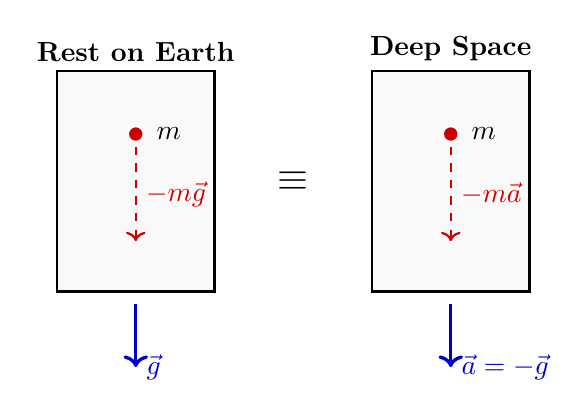
\begin{tikzpicture}[scale=0.8]
  % Left Box: Gravitational Field
  \draw[thick, fill=gray!5] (0,0) rectangle (2.5, 3.5);
  \node[above, font=\bfseries] at (1.25, 3.5) {Rest on Earth};
  \draw[->, very thick, blue!80!black] (1.25, -0.2) -- (1.25, -1.2) node[right] {$\vec{g}$};
  \fill[red!80!black] (1.25, 2.5) circle (3pt) node[right=4pt, text=black] {$m$};
  \draw[->, thick, dashed, red!80!black] (1.25, 2.3) -- (1.25, 0.8) node[midway, right] {$-m\vec{g}$};
  \draw[thick] (0.2, 0) -- (2.3, 0); % Floor emphasis

  % Right Box: Uniform Acceleration
  \begin{scope}[shift={(5,0)}]
    \draw[thick, fill=gray!5] (0,0) rectangle (2.5, 3.5);
    \node[above, font=\bfseries] at (1.25, 3.5) {Deep Space};
    \draw[->, very thick, blue!80!black] (1.25, -0.2) -- (1.25, -1.2) node[right] {$\vec{a} = -\vec{g}$};
    \fill[red!80!black] (1.25, 2.5) circle (3pt) node[right=4pt, text=black] {$m$};
    \draw[->, thick, dashed, red!80!black] (1.25, 2.3) -- (1.25, 0.8) node[midway, right] {$-m\vec{a}$};
    \draw[thick] (0.2, 0) -- (2.3, 0); % Floor emphasis
  \end{scope}

  % Equivalence symbol
  \node[font=\Large\bfseries] at (3.75, 1.75) {$\equiv$};
\end{tikzpicture}
\end{center}



\subsection*{The Einstein (EEP) and Strong (SEP) Equivalence Principles}
EEP states no local experiment can distinguish uniform acceleration from a gravitational field. Physics locally reduces to special relativity.
SEP extends this to all laws, including gravity itself.

\subsection*{From Equivalence to Geometry}
Gravity isn't a force; "unaccelerated" paths are redefined as freely-falling. Global inertial frames don't exist due to tidal forces. We define \textbf{locally inertial frames} modeled as a \textbf{differentiable manifold}.

% \usetikzlibrary{calc, positioning}
% \usepackage{amsmath}

\begin{center}
\begin{minipage}{0.48\textwidth}
\begin{center}
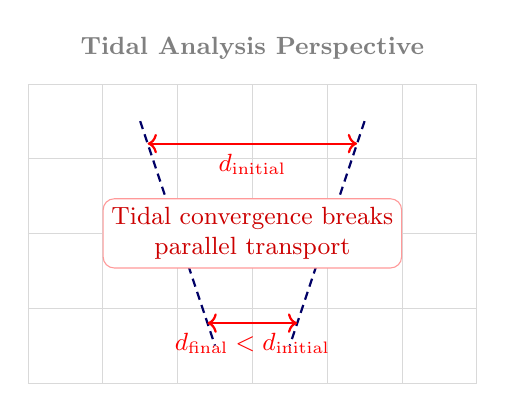
\begin{tikzpicture}[scale=0.95]
  % ----- Left Side: Tidal Analysis Grid -----
  % Rigid Cartesian Grid
  \draw[step=1cm, gray!30, very thin] (-3, 0) grid (3, 4);
  \node[gray, above, font=\bfseries\small] at (0, 4.2) {Tidal Analysis Perspective};

  % Falling paths (dashed trajectories)
  \draw[thick, blue!40!black, densely dashed] (-1.5, 3.5) -- (-0.5, 0.5);
  \draw[thick, blue!40!black, densely dashed] (1.5, 3.5) -- (0.5, 0.5);

  % Tidal effect annotations
  \draw[<->, thick, red] (-1.4, 3.2) -- (1.4, 3.2) node[midway, below, font=\small] {$d_{\text{initial}}$};
  \draw[<->, thick, red] (-0.6, 0.8) -- (0.6, 0.8) node[midway, below, font=\small] {$d_{\text{final}} < d_{\text{initial}}$};
  
  \node[fill=white, inner sep=3pt, draw=red!40, rounded corners, align=center, text=red!80!black, font=\small] at (0, 2) {Tidal convergence breaks \\ parallel transport};
\end{tikzpicture}
\end{center}
\end{minipage}
\hfill
\begin{minipage}{0.48\textwidth}
\begin{center}
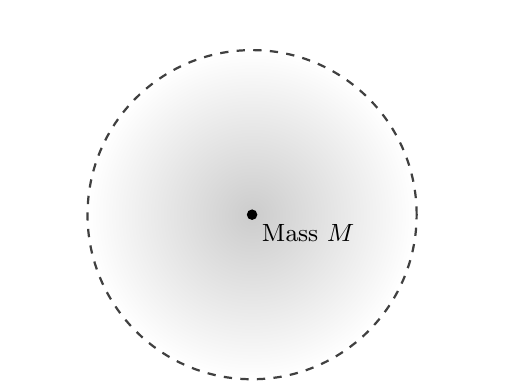
\begin{tikzpicture}[scale=0.95]
  % ----- Right Side: Gravitational Source Circle -----
  % Invisible bounding box matching the height of the left grid to maintain perfect baseline alignment
  \useasboundingbox (-3, 0) rectangle (3, 4.5);
  
  % Centered Gravitational Source (shifted vertically to center elegantly next to the grid)
  \begin{scope}[shift={(0, 2)}]
    \shade[inner color=gray!40, outer color=white] (0, 0) circle (2.2);
    \draw[thick, dashed, darkgray] (0, 0) circle (2.2);
    \fill (0, 0) circle (2pt) node[below right, font=\small] {Mass $M$};
  \end{scope}
\end{tikzpicture}
\end{center}
\end{minipage}
\end{center}

\subsection*{Prediction: Gravitational Redshift}
Accelerating rockets in flat spacetime separated by $z$:

1. Emitted photon wavelength $\lambda_0$ travels distance $z$, taking $\Delta t \approx z/c$.


2. Velocity increases by $\Delta v = a \Delta t = az/c$.


3. Doppler shift yields:
\begin{equation} \frac{\Delta \lambda}{\lambda_0} = \frac{\lambda_1 - \lambda_0}{\lambda_0} \approx \frac{\Delta v}{c} \end{equation}
\begin{equation} \frac{\Delta \lambda}{\lambda_0} = \frac{(az/c)}{c} = \frac{az}{c^2} \end{equation}


\begin{equation} \frac{\Delta \lambda}{\lambda_0} = \frac{a_g z}{c^2} \end{equation}
Using $a_g \approx \Delta \Phi / z$, we get:
\begin{equation} \frac{\Delta \lambda}{\lambda_0} \approx \Delta \Phi \end{equation}

\begin{center}
\begin{minipage}{0.48\textwidth}
\begin{center}
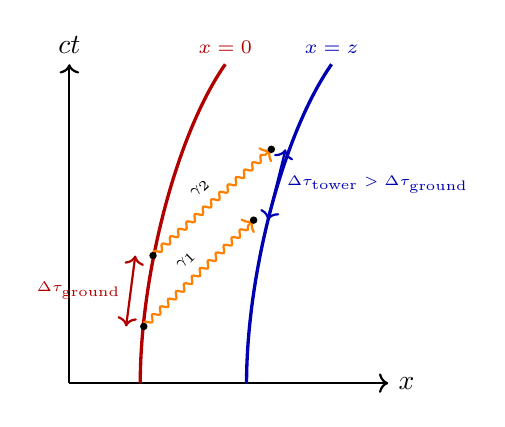
\begin{tikzpicture}[scale=0.9]
  % ----- Left Side: Spacetime Diagram -----
  % Axes
  \draw[->, thick] (0,0) -- (0, 4.5) node[above] {$ct$};
  \draw[->, thick] (0,0) -- (4.5, 0) node[right] {$x$};

  % Worldlines (Rindler-like curving)
  \draw[very thick, red!70!black] (1, 0) .. controls (1, 1.5) and (1.5, 3.5) .. (2.2, 4.5) 
    node[above, font=\scriptsize] {$x=0$};
  \draw[very thick, blue!70!black] (2.5, 0) .. controls (2.5, 1.5) and (3.0, 3.5) .. (3.7, 4.5) 
    node[above, font=\scriptsize] {$x=z$};

  % Photon 1
  \coordinate (E1) at (1.05, 0.8);
  \coordinate (R1) at (2.6, 2.3);
  \draw[->, thick, orange, decorate, decoration={snake, amplitude=1pt, segment length=4pt, post length=2pt}] 
    (E1) -- (R1) node[midway, sloped, above=1pt, text=black, font=\tiny] {$\gamma_1$};
  \fill (E1) circle (1.5pt); \fill (R1) circle (1.5pt);

  % Photon 2
  \coordinate (E2) at (1.18, 1.8);
  \coordinate (R2) at (2.85, 3.3);
  \draw[->, thick, orange, decorate, decoration={snake, amplitude=1pt, segment length=4pt, post length=2pt}] 
    (E2) -- (R2) node[midway, sloped, above=1pt, text=black, font=\tiny] {$\gamma_2$};
  \fill (E2) circle (1.5pt); \fill (R2) circle (1.5pt);

  % Time intervals
  \draw[<->, thick, red!70!black] (0.8, 0.8) -- (0.93, 1.8) 
    node[midway, left, font=\tiny] {$\Delta \tau_{\text{ground}}$};
  \draw[<->, thick, blue!70!black] (2.8, 2.3) -- (3.05, 3.3) 
    node[midway, right, font=\tiny] {$\Delta \tau_{\text{tower}} > \Delta \tau_{\text{ground}}$};
\end{tikzpicture}
\end{center}
\end{minipage}
\hfill
\begin{minipage}{0.48\textwidth}
\begin{center}
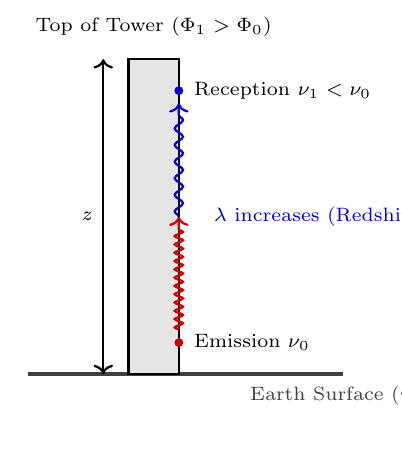
\begin{tikzpicture}[scale=0.8]
  % ----- Right Side: Physical Tower Diagram -----
  % Establish matching vertical bounds to ensure perfect alignment
  \useasboundingbox (-2, -0.8) rectangle (3.5, 5.5);

  % Ground Surface
  \draw[ultra thick, darkgray] (-2,0) -- (3,0) node[below, font=\scriptsize] {Earth Surface ($\Phi_0$)};
  
  % Tower
  \draw[thick, fill=gray!20] (-0.4, 0) rectangle (0.4, 5);
  \draw[<->, thick] (-0.8, 0) -- (-0.8, 5) node[midway, left, font=\scriptsize] {$z$};
  \node[above, font=\scriptsize] at (0, 5.2) {Top of Tower ($\Phi_1 > \Phi_0$)};

  % Photon Emission (Bottom)
  \fill[red!80!black] (0.4, 0.5) circle (2pt) node[right=2pt, text=black, font=\scriptsize] {Emission $\nu_0$};
  
  % Photon Reception (Top)
  \fill[blue!80!black] (0.4, 4.5) circle (2pt) node[right=2pt, text=black, font=\scriptsize] {Reception $\nu_1 < \nu_0$};

  % Wavelength stretch visualization
  \draw[->, thick, decorate, decoration={snake, amplitude=1.5pt, segment length=3pt, post length=4pt}, red!80!black] 
    (0.4, 0.7) -- (0.4, 2.5);
  \draw[->, thick, decorate, decoration={snake, amplitude=1.5pt, segment length=6pt, post length=4pt}, blue!80!black] 
    (0.4, 2.5) -- (0.4, 4.3);
    
  \node[right, font=\scriptsize, text=blue!80!black] at (0.8, 2.5) {$\lambda$ increases (Redshift)};
\end{tikzpicture}
\end{center}
\end{minipage}
\end{center}

\section{What Is a Manifold?}
A differentiable manifold locally resembles $\mathbb{R}^n$.
Examples: $\mathbb{R}^n$, $n$-sphere $S^n$, $n$-torus $T^n$, Riemann Surfaces, Lie Groups, Direct Products.


% DIAGRAM 2: Surfaces with genus 0, 1, and 2
% SKIPPED: Not suitable for TikZ (highly detailed 3D organic shapes).

% DIAGRAM 4: Single cone (manifold) and line segment (manifold with boundary)
% SKIPPED: Not suitable for TikZ (Redundant with general 3D CAD modeling tools).


\subsection*{Formal Definition}


\begin{center}
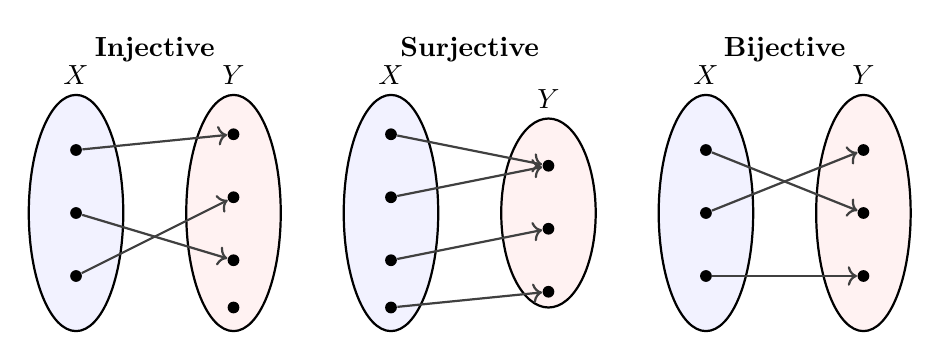
\begin{tikzpicture}[scale=1]
  \tikzset{dot/.style={circle, fill=black, inner sep=1.5pt}}
  
  % Injective
  \begin{scope}[shift={(0,0)}]
    \node[above, font=\bfseries] at (1, 2.8) {Injective};
    \draw[thick, fill=blue!5] (0, 1) ellipse (0.6 and 1.5) node[above=1.5cm] {$X$};
    \draw[thick, fill=red!5] (2, 1) ellipse (0.6 and 1.5) node[above=1.5cm] {$Y$};
    \node[dot] (a1) at (0, 1.8) {}; \node[dot] (a2) at (0, 1) {}; \node[dot] (a3) at (0, 0.2) {};
    \node[dot] (b1) at (2, 2) {}; \node[dot] (b2) at (2, 1.2) {}; \node[dot] (b3) at (2, 0.4) {}; \node[dot] (b4) at (2, -0.2) {};
    \draw[->, thick, darkgray] (a1) -- (b1); 
    \draw[->, thick, darkgray] (a2) -- (b3); 
    \draw[->, thick, darkgray] (a3) -- (b2);
  \end{scope}

  % Surjective
  \begin{scope}[shift={(4,0)}]
    \node[above, font=\bfseries] at (1, 2.8) {Surjective};
    \draw[thick, fill=blue!5] (0, 1) ellipse (0.6 and 1.5) node[above=1.5cm] {$X$};
    \draw[thick, fill=red!5] (2, 1) ellipse (0.6 and 1.2) node[above=1.2cm] {$Y$};
    \node[dot] (c1) at (0, 2) {}; \node[dot] (c2) at (0, 1.2) {}; \node[dot] (c3) at (0, 0.4) {}; \node[dot] (c4) at (0, -0.2) {};
    \node[dot] (d1) at (2, 1.6) {}; \node[dot] (d2) at (2, 0.8) {}; \node[dot] (d3) at (2, 0) {};
    \draw[->, thick, darkgray] (c1) -- (d1); 
    \draw[->, thick, darkgray] (c2) -- (d1); 
    \draw[->, thick, darkgray] (c3) -- (d2); 
    \draw[->, thick, darkgray] (c4) -- (d3);
  \end{scope}

  % Bijective
  \begin{scope}[shift={(8,0)}]
    \node[above, font=\bfseries] at (1, 2.8) {Bijective};
    \draw[thick, fill=blue!5] (0, 1) ellipse (0.6 and 1.5) node[above=1.5cm] {$X$};
    \draw[thick, fill=red!5] (2, 1) ellipse (0.6 and 1.5) node[above=1.5cm] {$Y$};
    \node[dot] (e1) at (0, 1.8) {}; \node[dot] (e2) at (0, 1) {}; \node[dot] (e3) at (0, 0.2) {};
    \node[dot] (f1) at (2, 1.8) {}; \node[dot] (f2) at (2, 1) {}; \node[dot] (f3) at (2, 0.2) {};
    \draw[->, thick, darkgray] (e1) -- (f2); 
    \draw[->, thick, darkgray] (e2) -- (f1); 
    \draw[->, thick, darkgray] (e3) -- (f3);
  \end{scope}
\end{tikzpicture}
\end{center}


\begin{center}
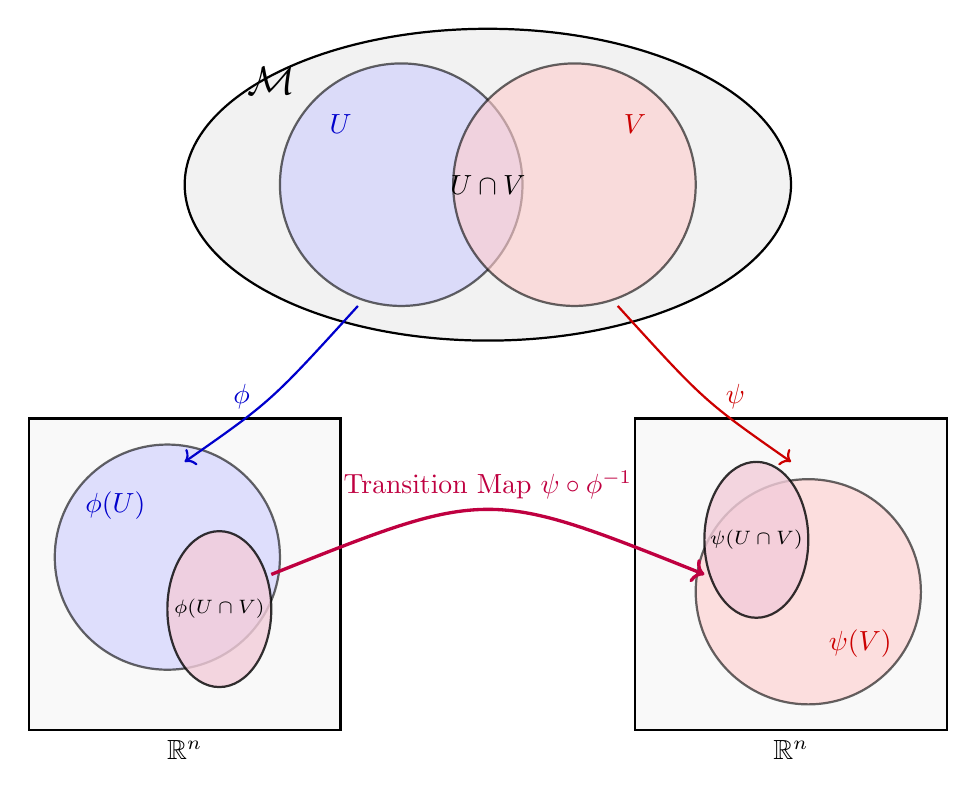
\begin{tikzpicture}[scale=1.1]
  % Manifold M
  \draw[thick, fill=gray!10] (0,0) ellipse (3.5 and 1.8);
  \node[font=\Large\bfseries] at (-2.5, 1.2) {$\mathcal{M}$};
  
  % Sets U and V
  \draw[thick, fill=blue!20, opacity=0.6] (-1, 0) circle (1.4);
  \node[blue!80!black, font=\bfseries] at (-1.7, 0.7) {$U$};
  
  \draw[thick, fill=red!20, opacity=0.6] (1, 0) circle (1.4);
  \node[red!80!black, font=\bfseries] at (1.7, 0.7) {$V$};
  
  % U intersect V (Manifold)
  \node[font=\bfseries] at (0, 0) {$U \cap V$};
  
  % Chart 1 (Left) - R^n space
  \begin{scope}[shift={(-3.5, -4.5)}]
    \draw[thick, fill=gray!5] (-1.8, -1.8) rectangle (1.8, 1.8);
    \node[below] at (0, -1.8) {$\mathbb{R}^n$};
    \draw[thick, fill=blue!20, opacity=0.6] (-0.2,0.2) circle (1.3);
    \node[blue!80!black] at (-0.8, 0.8) {$\phi(U)$};
    % Image of intersection
    \draw[thick, fill=purple!20, opacity=0.8] (0.4,-0.4) ellipse (0.6 and 0.9);
    \node[font=\scriptsize, align=center] at (0.4, -0.4) {$\phi(U \cap V)$};
  \end{scope}

  % Chart 2 (Right) - R^n space
  \begin{scope}[shift={(3.5, -4.5)}]
    \draw[thick, fill=gray!5] (-1.8, -1.8) rectangle (1.8, 1.8);
    \node[below] at (0, -1.8) {$\mathbb{R}^n$};
    \draw[thick, fill=red!20, opacity=0.6] (0.2,-0.2) circle (1.3);
    \node[red!80!black] at (0.8, -0.8) {$\psi(V)$};
    % Image of intersection
    \draw[thick, fill=purple!20, opacity=0.8] (-0.4,0.4) ellipse (0.6 and 0.9);
    \node[font=\scriptsize, align=center] at (-0.4, 0.4) {$\psi(U \cap V)$};
  \end{scope}
  
  % Mappings from Manifold to R^n
  \draw[->, thick, blue!80!black] (-1.5, -1.4) .. controls (-2.5, -2.5) .. (-3.5, -3.2) node[midway, left=4pt] {$\phi$};
  \draw[->, thick, red!80!black] (1.5, -1.4) .. controls (2.5, -2.5) .. (3.5, -3.2) node[midway, right=4pt] {$\psi$};
  
  % Transition Map between R^n charts
  \draw[->, very thick, purple] (-2.5, -4.5) .. controls (0, -3.5) .. (2.5, -4.5) node[midway, above] {Transition Map $\psi \circ \phi^{-1}$};
\end{tikzpicture}
\end{center}



% DIAGRAM 8: Circle covered by two overlapping open charts
% SKIPPED: Not suitable for TikZ (Redundant due to the comprehensive transition map diagram above).


\subsubsection*{Stereographic Projection on $S^2$}
Let $S^2$ be $(x^1)^2 + (x^2)^2 + (x^3)^2 = 1$.


\begin{center}
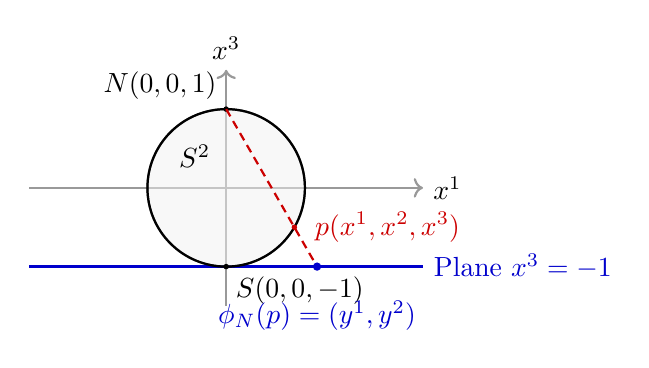
\begin{tikzpicture}[scale=1.0]
  % Axes
  \draw[->, thick, gray!80] (-2.5, 0) -- (2.5, 0) node[right, text=black] {$x^1$};
  \draw[->, thick, gray!80] (0, -1.5) -- (0, 1.5) node[above, text=black] {$x^3$};

  % Projection Plane x^3 = -1
  \draw[very thick, blue!80!black] (-2.5, -1) -- (2.5, -1) node[right] {Plane $x^3 = -1$};

  % Sphere S^2 cross-section (S^1)
  \draw[thick, fill=gray!10, opacity=0.5] (0,0) circle (1);
  \draw[thick] (0,0) circle (1);
  \node at (-0.4, 0.4) {$S^2$};
  
  % Poles
  \fill[black] (0, 1) circle (1pt) node[above left] {$N (0,0,1)$};
  \fill[black] (0, -1) circle (1pt) node[below right] {$S (0,0,-1)$};

  % Point P on the sphere (picking an arbitrary point)
  \coordinate (P) at (0.866, -0.5); % (sin(60), -cos(60))
  \fill[red!80!black] (P) circle (1pt) node[right=4pt] {$p (x^1, x^2, x^3)$};

  % Projection line from N through P to the plane
  % The line intersects z=-1 at x = 2/sqrt(3) ≈ 1.154
  \coordinate (Proj) at (1.154, -1);
  \draw[thick, densely dashed, red!80!black] (0,1) -- (Proj);
  
  % Projected point on the plane
  \fill[blue!80!black] (Proj) circle (1.5pt) node[below=9pt] {$\phi_N(p) = (y^1, y^2)$};
\end{tikzpicture}
\end{center}


\begin{equation} (y^1, y^2) = \phi_N(x^1, x^2, x^3) = \left( \frac{2x^1}{1-x^3}, \frac{2x^2}{1-x^3} \right) \end{equation}
\textbf{Chart 2 (South Pole $S$ excluded):} Projects to plane $x^3=+1$ with coordinates $(z^1, z^2)$.
\begin{equation} (z^1, z^2) = \phi_S(x^1, x^2, x^3) = \left( \frac{2x^1}{1+x^3}, \frac{2x^2}{1+x^3} \right) \end{equation}

\subsubsection*{Derivation: Transition Map for $S^2$}
Invert $\phi_N$: Let $Y^2 = (y^1)^2 + (y^2)^2$.


$$ Y^2 = \frac{4(x^1)^2 + 4(x^2)^2}{(1-x^3)^2} = \frac{4(1-x^3)(1+x^3)}{(1-x^3)^2} = \frac{4(1+x^3)}{1-x^3} $$

$$ Y^2(1-x^3) = 4(1+x^3) \implies x^3 = \frac{Y^2 - 4}{Y^2 + 4} $$

$$ 1 - x^3 = \frac{8}{Y^2 + 4} $$

$$ x^1 = \frac{y^1 (1-x^3)}{2} = \frac{4y^1}{Y^2 + 4}, \quad x^2 = \frac{4y^2}{Y^2 + 4} $$


Apply $\phi_S$:


$$ (z^1, z^2) = \left( \frac{2x^1}{1+x^3}, \frac{2x^2}{1+x^3} \right) $$

$$ 1 + x^3 = \frac{2Y^2}{Y^2 + 4} $$

$$ z^1 = \frac{4y^1}{(y^1)^2 + (y^2)^2}, \quad z^2 = \frac{4y^2}{(y^1)^2 + (y^2)^2} $$

Transition map is $C^\infty$ except at $(0,0)$ (South Pole, excluded).

\subsection*{The Chain Rule}


\begin{center}
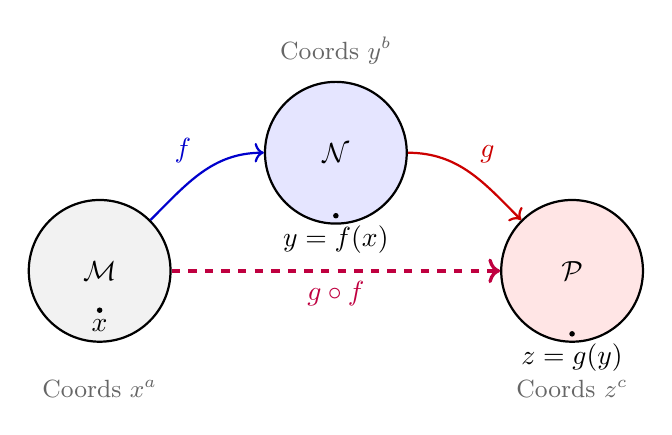
\begin{tikzpicture}[scale=1.0]
  % Spaces
  \node (M) at (0,0) [circle, draw, thick, fill=gray!10, minimum size=1.8cm] {$\mathcal{M}$};
  \node (N) at (3,1.5) [circle, draw, thick, fill=blue!10, minimum size=1.8cm] {$\mathcal{N}$};
  \node (P) at (6,0) [circle, draw, thick, fill=red!10, minimum size=1.8cm] {$\mathcal{P}$};

  % Mappings
  \draw[->, thick, blue!80!black] (M) to[out=45, in=180] node[midway, above left] {$f$} (N);
  \draw[->, thick, red!80!black] (N) to[out=0, in=135] node[midway, above right] {$g$} (P);
  \draw[->, very thick, dashed, purple] (M) to[out=0, in=180] node[midway, below] {$g \circ f$} (P);
  
  % Points and Coordinates
  \fill[black] (0.0, -0.5) circle (1pt) node[below] {$x$};
  \fill[black] (3, 0.7) circle (1pt) node[below] {$y = f(x)$};
  \fill[black] (6.0, -0.8) circle (1pt) node[below] {$z = g(y)$};
  
  % Coordinate system labels
  \node[font=\small, text=gray!80!black] at (0, -1.5) {Coords $x^a$};
  \node[font=\small, text=gray!80!black] at (3, 2.8) {Coords $y^b$};
  \node[font=\small, text=gray!80!black] at (6, -1.5) {Coords $z^c$};
\end{tikzpicture}
\end{center}

\begin{equation} \frac{\partial (g \circ f)^c}{\partial x^a} = \sum_{b=1}^n \frac{\partial f^b}{\partial x^a} \frac{\partial g^c}{\partial y^b} \end{equation}
\begin{equation} \frac{\partial}{\partial x^a} = \sum_{b=1}^n \frac{\partial y^b}{\partial x^a} \frac{\partial}{\partial y^b} \end{equation}

\section{Vectors Again}


$T_p$ is defined as the set of directional derivative operators at $p$.
Linearity: $X = a \frac{d}{d\lambda_1} + b \frac{d}{d\lambda_2}$.
Leibniz Rule:
\begin{align*}
X(fg) &= \left(a \frac{d}{d\lambda_1} + b \frac{d}{d\lambda_2}\right) (fg) \\
&= f \left( a \frac{dg}{d\lambda_1} + b \frac{dg}{d\lambda_2} \right) + g \left( a \frac{df}{d\lambda_1} + b \frac{df}{d\lambda_2} \right) = f (X(g)) + g (X(f))
\end{align*}

\subsection*{The Coordinate Basis}
Partial derivatives $\{\partial_\mu\}$ form a basis.


\begin{center}
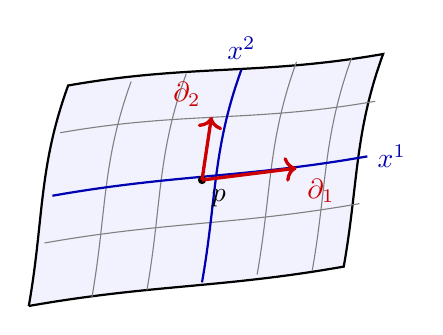
\begin{tikzpicture}[scale=1.0]
  % Define point p
  \coordinate (P) at (2.2, 1.6);

  % Curved surface
  \draw[thick, fill=blue!5] (0,0) to[out=10, in=190] (4,0.5) 
        to[out=80, in=250] (4.5,3.2) 
        to[out=190, in=10] (0.5,2.8) 
        to[out=250, in=80] (0,0);
        
  % Coordinate lines (thin gray)
  \draw[gray, thin] (0.8, 0.1) to[out=80, in=250] (1.3, 2.85);
  \draw[gray, thin] (1.5, 0.2) to[out=80, in=250] (2.0, 2.95);
  \draw[gray, thin] (2.9, 0.4) to[out=80, in=250] (3.4, 3.1);
  \draw[gray, thin] (3.6, 0.45) to[out=80, in=250] (4.1, 3.15);

  \draw[gray, thin] (0.2, 0.8) to[out=10, in=190] (4.2, 1.3);
  \draw[gray, thin] (0.4, 2.2) to[out=10, in=190] (4.4, 2.6);

  % Highlighted coordinate lines passing through p
  % x^1 curve
  \draw[blue!70!black, thick] (0.3, 1.4) to[out=10, in=190] (4.3, 1.9) node[right] {$x^1$};
  % x^2 curve
  \draw[blue!70!black, thick] (2.2, 0.3) to[out=80, in=250] (2.7, 3.0) node[above] {$x^2$};

  % Mark point p
  \fill[black] (P) circle (1.5pt) node[below right] {$p$};

  % Tangent basis vectors
  \draw[->, very thick, red!80!black] (P) -- ++(1.2, 0.15) node[below right] {$\partial_1$};
  \draw[->, very thick, red!80!black] (P) -- ++(0.12, 0.8) node[above left] {$\partial_2$};

\end{tikzpicture}
\end{center}



\textbf{Derivation:}
\begin{equation}
\begin{split}
\frac{d}{d\lambda}(f) &= \frac{d}{d\lambda} [(f \circ \phi^{-1}) \circ (\phi \circ \gamma)] \\
&= \frac{dx^\mu}{d\lambda} \frac{\partial f}{\partial x^\mu}
\end{split}
\end{equation}


$$\frac{d}{d\lambda} = \frac{dx^\mu}{d\lambda} {\partial_\mu }$$

\subsection*{Transformation Properties}
Basis Vector Transformation:
\begin{equation} \partial_{\mu'} = \frac{\partial x^\mu}{\partial x^{\mu'}} \partial_\mu \end{equation}
Vector Component Transformation:


$$ V = V^{\mu'} \left( \frac{\partial x^\mu}{\partial x^{\mu'}} \partial_\mu \right) \implies V^\mu = V^{\mu'} \frac{\partial x^\mu}{\partial x^{\mu'}} $$


\begin{equation} V^{\mu'} = \frac{\partial x^{\mu'}}{\partial x^\mu} V^\mu \end{equation}


\begin{center}
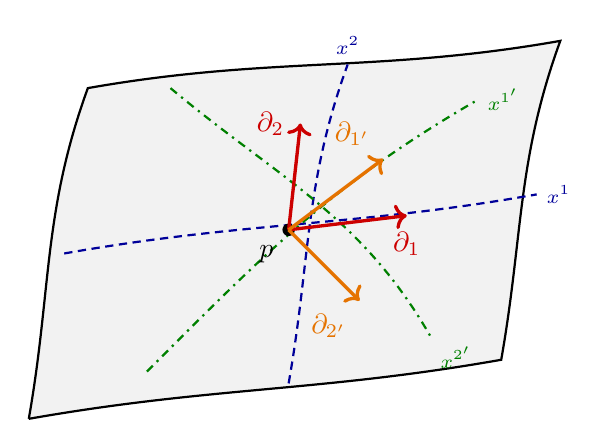
\begin{tikzpicture}[scale=1.5]
  % Define point p
  \coordinate (P) at (2.2, 1.6);

  % Curved surface patch
  \draw[thick, fill=gray!10] (0,0) to[out=10, in=190] (4,0.5) 
        to[out=80, in=250] (4.5,3.2) 
        to[out=190, in=10] (0.5,2.8) 
        to[out=250, in=80] (0,0);

  % Grid 1 (x^\mu) lines
  \draw[blue!60!black, thick, densely dashed] (0.3, 1.4) to[out=10, in=190] (4.3, 1.9) node[right, font=\scriptsize] {$x^1$};
  \draw[blue!60!black, thick, densely dashed] (2.2, 0.3) to[out=80, in=250] (2.7, 3.0) node[above, font=\scriptsize] {$x^2$};

  % Grid 2 (x^{\mu'}) lines
  \draw[green!50!black, thick, dash dot] (1.0, 0.4) to[out=45, in=210] (3.8, 2.7) node[right, font=\scriptsize] {$x^{1'}$};
  \draw[green!50!black, thick, dash dot] (1.2, 2.8) to[out=-40, in=120] (3.4, 0.7) node[below right, font=\scriptsize] {$x^{2'}$};

  % Mark point p
  \fill[black] (P) circle (1.5pt) node[below left=2pt] {$p$};

  % Basis Vectors for Grid 1 (Red)
  \draw[->, very thick, red!80!black] (P) -- ++(1.0, 0.12) node[below=2pt] {$\partial_1$};
  \draw[->, very thick, red!80!black] (P) -- ++(0.1, 0.9) node[left=2pt] {$\partial_2$};

  % Basis Vectors for Grid 2 (Orange)
  \draw[->, very thick, orange!90!black] (P) -- ++(0.8, 0.6) node[above left=1pt] {$\partial_{1'}$};
  \draw[->, very thick, orange!90!black] (P) -- ++(0.6, -0.6) node[below left=1pt] {$\partial_{2'}$};

\end{tikzpicture}
\end{center}

\subsection*{The Commutator (Lie Bracket)}
\begin{equation} [X, Y](f) \equiv X(Y(f)) - Y(X(f)) \end{equation}
\begin{align*}
[X, Y]^\nu &= X(Y^\mu \partial_\mu x^\nu) - Y(X^\lambda \partial_\lambda x^\nu) \\
&= X(Y^\nu) - Y(X^\nu) \\
&= (X^\lambda \partial_\lambda) Y^\nu - (Y^\mu \partial_\mu) X^\nu
\end{align*}
\begin{equation} [X, Y]^\nu = X^\lambda \partial_\lambda Y^\nu - Y^\lambda \partial_\lambda X^\nu \end{equation}

\section{Tensors Again}
\subsection*{Dual Vectors (One-Forms)}


$T_p^*$ maps $T_p \to \mathbb{R}$.
\begin{equation} df\left(\frac{d}{d\lambda}\right) = \frac{df}{d\lambda} \end{equation}

\subsection*{Basis and Components}


$\{dx^\mu\}$ forms the dual basis to $\{\partial_\nu\}$.


$$ dx^\mu (\partial_\nu) \equiv \partial_\nu (x^\mu) = \frac{\partial x^\mu}{\partial x^\nu} = \delta^\mu_\nu $$


\begin{equation} dx^\mu (\partial_\nu) = \delta^\mu_\nu \end{equation}

\subsection*{Transformation Properties}
\begin{equation} dx^{\mu'} = \frac{\partial x^{\mu'}}{\partial x^\mu} dx^\mu \end{equation}


$$ \omega = \omega_{\mu'} \left( \frac{\partial x^{\mu'}}{\partial x^\mu} dx^\mu \right) $$


\begin{equation} \omega_{\nu'} = \frac{\partial x^\mu}{\partial x^{\nu'}} \omega_\mu \end{equation}

\subsection*{General Tensors}
\begin{equation} T = {T^{\mu_1 \dots \mu_k}}*{\nu_1 \dots \nu_l} \partial*{\mu_1} \otimes \dots \otimes \partial_{\mu_k} \otimes dx^{\nu_1} \otimes \dots \otimes dx^{\nu_l} \end{equation}
\begin{equation} {T^{\mu_1 \dots \mu_k}}*{\nu_1 \dots \nu_l} = T(dx^{\mu_1}, \dots, dx^{\mu_k}, \partial*{\nu_1}, \dots, \partial_{\nu_l}) \end{equation}
\begin{equation} {T^{\mu'_1 \dots \mu'*k}}*{\nu'_1 \dots \nu'_l} = \frac{\partial x^{\mu'_1}}{\partial x^{\mu_1}} \dots \frac{\partial x^{\nu_1}}{\partial x^{\nu'*1}} \dots {T^{\mu_1 \dots \mu_k}}*{\nu_1 \dots \nu_l} \end{equation}

\subsection*{Example: Transforming a (0,2) Tensor}
\begin{equation} S = S_{\mu\nu} dx^\mu dx^\nu = 1 , (dx)^2 + x^2 (dy)^2 \end{equation}
Coordinate change: $x' = 2x/y, y' = y/2$. Inverting gives $y = 2y', x = x'y'$.
Differentials:


$$ dx = y' dx' + x' dy', \quad dy = 2 dy' $$


Substitute into $S$:


$$ S = (y'dx' + x'dy')^2 + (x'y')^2 (2dy')^2 $$

$$ S = (y')^2 (dx')^2 + x'y' (dx'dy' + dy'dx') + \left[ (x')^2 + 4(x'y')^2 \right] (dy')^2 $$


\begin{equation} \label{S_transform} S_{\mu'\nu'} = \begin{pmatrix} (y')^2 & x'y' \ x'y' & (x')^2 + 4(x'y')^2 \end{pmatrix} \end{equation}
Verifying via full transformation law:
\begin{equation} S_{\mu'\nu'} = \frac{\partial x^\mu}{\partial x^{\mu'}} \ \frac{\partial x^\nu}{\partial x^{\nu'}} , S_{\mu \nu} \end{equation}
\begin{align*}
S_{x'x'} &= (y')(y')(1) = (y')^2 \\
S_{x'y'} &= (y')(x')(1) = x'y' \\
S_{y'y'} &= (x')(x')(1) + (2)(2)(x^2) = (x')^2 + 4(x'y')^2
\end{align*}

\subsection*{The Failure of Partial Derivatives}


$\partial_\mu W_\nu$ is not a tensor.


$$ \partial_{\mu'} W_{\nu'} = \frac{\partial}{\partial x^{\mu'}} \left( \frac{\partial x^\nu}{\partial x^{\nu'}} W_\nu \right) $$

$$ \partial_{\mu'} W_{\nu'} = \left( \frac{\partial x^\mu}{\partial x^{\mu'}} \frac{\partial^2 x^\nu}{\partial x^\mu \partial x^{\nu'}} \right) W_\nu + \frac{\partial x^\nu}{\partial x^{\nu'}} \left( \frac{\partial x^\mu}{\partial x^{\mu'}} \partial_\mu W_\nu \right) $$


\begin{equation} \partial_{\mu'} W_{\nu'} = \frac{\partial x^\mu}{\partial x^{\mu'}} \frac{\partial x^\nu}{\partial x^{\nu'}} (\partial_\mu W_\nu) + W_\nu \frac{\partial^2 x^\nu}{\partial x^{\mu'} \partial x^{\nu'}} \end{equation}
The second term vanishes only for linear transformations. This motivates the \textbf{covariant derivative}.

\section{The Metric}
The metric $g_{\mu\nu}$ is a nondegenerate, symmetric (0,2) tensor.
\begin{equation} g^{\mu\nu} g_{\nu\sigma} = \delta^\mu_\sigma \end{equation}
\begin{equation} ds^2 = g_{\mu\nu} dx^\mu dx^\nu \end{equation}

\subsection*{Example: Flat Space in Spherical Coordinates}
$x = r \sin\theta \cos\phi, \quad y = r \sin\theta \sin\phi, \quad z = r \cos\theta$
Differentials:
\begin{align*}
dx &= (\sin\theta\cos\phi)dr + (r\cos\theta\cos\phi)d\theta - (r\sin\theta\sin\phi)d\phi \\
dy &= (\sin\theta\sin\phi)dr + (r\cos\theta\sin\phi)d\theta + (r\sin\theta\cos\phi)d\phi \\
dz &= (\cos\theta)dr - (r\sin\theta)d\theta
\end{align*}
Summing $(dx)^2 + (dy)^2 + (dz)^2$:
\begin{align*}
ds^2 &= \left[ \sin^2\theta dr^2 + r^2\cos^2\theta d\theta^2 + r^2\sin^2\theta d\phi^2 + 2r\sin\theta\cos\theta dr d\theta \right] \\
& \quad + \left[ \cos^2\theta dr^2 - 2r\sin\theta\cos\theta dr d\theta + r^2\sin^2\theta d\theta^2 \right]
\end{align*}
\begin{equation} ds^2 = dr^2 + r^2 d\theta^2 + r^2\sin^2\theta d\phi^2 \end{equation}
For the 2-sphere $S^2$ (constant $r=R$):
\begin{equation} ds^2 = R^2 d\theta^2 + R^2\sin^2\theta d\phi^2 \end{equation}

\begin{center}
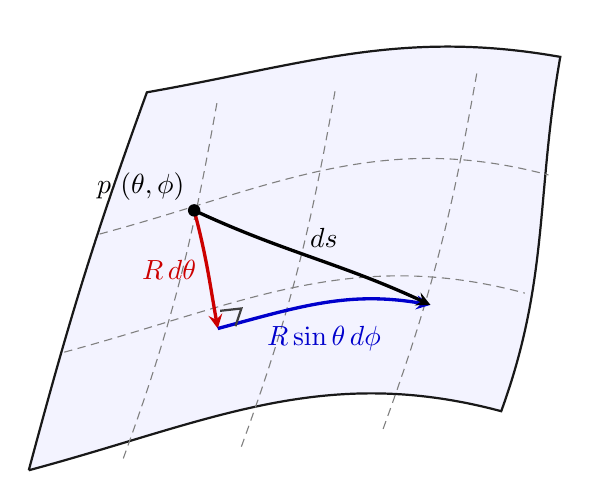
\begin{tikzpicture}[scale=1.5]
  % Draw a curved patch of the 2-sphere
  \draw[thick, fill=blue!5, opacity=0.9] (0,0) to[out=15, in=165] (4,0.5) 
        to[out=70, in=260] (4.5, 3.5) 
        to[out=170, in=10] (1, 3.2) 
        to[out=250, in=75] (0,0);
        
  % Grid lines (Lines of constant theta and phi) to imply curvature
  \draw[gray, thin, densely dashed] (0.8, 0.1) to[out=70, in=260] (1.6, 3.15);
  \draw[gray, thin, densely dashed] (1.8, 0.2) to[out=70, in=260] (2.6, 3.25);
  \draw[gray, thin, densely dashed] (3.0, 0.35) to[out=70, in=260] (3.8, 3.4);
  
  \draw[gray, thin, densely dashed] (0.3, 1.0) to[out=15, in=165] (4.2, 1.5);
  \draw[gray, thin, densely dashed] (0.6, 2.0) to[out=15, in=165] (4.4, 2.5);

  % Infinitesimal right-triangle points
  % A = Point p (theta, phi)
  % B = Point displaced by d\theta (theta + d\theta, phi)
  % C = Point displaced by d\theta and d\phi (theta + d\theta, phi + d\phi)
  \coordinate (A) at (1.4, 2.2);
  \coordinate (B) at (1.6, 1.2);
  \coordinate (C) at (3.4, 1.4);

  % d(theta) side (meridian - arc length R d\theta)
  \draw[very thick, red!80!black, -stealth] (A) to[out=285, in=100] (B);
  \node[left, red!80!black] at (1.5, 1.7) {$R \, d\theta$};

  % d(phi) side (parallel of latitude - arc length R \sin\theta d\phi)
  \draw[very thick, blue!80!black, -stealth] (B) to[out=15, in=170] (C);
  \node[below, blue!80!black] at (2.5, 1.3) {$R \sin\theta \, d\phi$};

  % ds side (hypotenuse - invariant interval)
  \draw[very thick, black, -stealth] (A) to[out=-25, in=155] (C);
  \node[above right, font=\bfseries] at (2.3, 1.8) {$ds$};

  % Mark the starting point
  \fill (A) circle (1.5pt) node[above left] {$p \ (\theta, \phi)$};

  % Fake right angle symbol (approximated for curved perspective)
  \draw[thick, darkgray] (1.75, 1.22) -- (1.8, 1.37) -- (1.62, 1.35);

\end{tikzpicture}
\end{center}

\subsection*{Locally Inertial Coordinates (LIC)}
In a LIC $x^{\hat{\mu}}$, gravity vanishes to first order:
\begin{align} g_{\hat{\mu}\hat{\nu}}(p) &= \eta_{\hat{\mu}\hat{\nu}} \ \partial_{\hat{\sigma}} g_{\hat{\mu}\hat{\nu}}(p) &= 0 \end{align}
Degrees of freedom (4D):

1. Zeroth Order: 16 parameters to fix 10 components.
2. First Order: 40 parameters to fix 40 components ($\partial_{\hat{\sigma}} g_{\hat{\mu}\hat{\nu}} = 0$).
3. Second Order: 80 parameters to fix 100 components ($\partial_{\hat{\rho}}\partial_{\hat{\sigma}} g_{\hat{\mu}\hat{\nu}} = 0$). Short by 20 parameters, defining the Riemann curvature tensor.



\textbf{Relative Velocity Example:}
In observer's LIC, $U^{\hat{\mu}} = (1, 0, 0, 0)$. Rocket $V^{\hat{\mu}} = (\gamma, \gamma v^1, \gamma v^2, \gamma v^3)$.


$$ \eta_{\hat{\mu}\hat{\nu}} U^{\hat{\mu}} V^{\hat{\nu}} = -\gamma $$

$$ v = \sqrt{1 - \gamma^{-2}} = \sqrt{1 - ( \eta_{\hat{\mu}\hat{\nu}} U^{\hat{\mu}} V^{\hat{\nu}} )^{-2}} $$

Covariant expression:
\begin{equation} v = \sqrt{1 - (g_{\mu\nu} U^\mu V^\nu)^{-2}} \end{equation}

\section{An Expanding Universe}
Robertson-Walker (RW) metric:
\begin{equation}\label{eq:rw-metric} ds^2 = -dt^2 + a^2(t)[(dx)^2 + (dy)^2 + (dz)^2] \end{equation}
For $a(t) = t^q$ ($0 < q < 1$):
\begin{equation} a(t) = t^q \end{equation}

\subsection*{Light Cones and Particle Horizon}
Null path ($ds^2=0$):


$$ 0 = -dt^2 + t^{2q} (dx)^2 \implies \frac{dx}{dt} = \pm t^{-q} $$


Justification via tangent vector $V = \frac{dx^\mu}{d\lambda} \partial_\mu$:
\begin{align*}
g(V,V) &= -1 \left(\frac{dt}{d\lambda}\right)^2 + a(t)^2 \left(\frac{dx}{d\lambda}\right)^2 = 0
\end{align*}
\begin{equation} -\left(\frac{dt}{d\lambda}\right)^2 + t^{2q} \left(\frac{dx}{d\lambda}\right)^2 = 0 \implies \left(\frac{dx}{dt}\right)^2 = t^{-2q} \end{equation}
Particle horizon integration:


$$ x(t) = \pm \int_{t_0}^{t} (t')^{-q} dt' = \pm \frac{t^{1-q}}{1-q} $$

\begin{center}
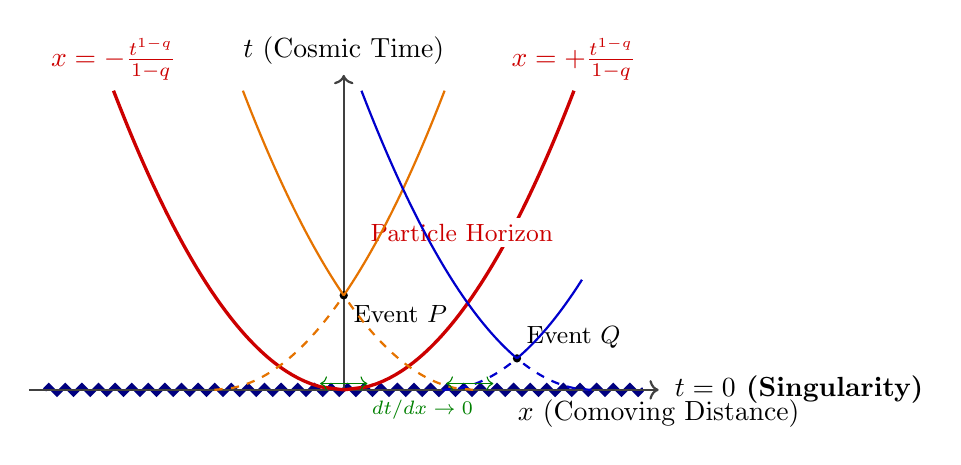
\begin{tikzpicture}[scale=1.0]
  % Singularity (Big Bang)
  \draw[ultra thick, decorate, decoration={zigzag, segment length=6pt, amplitude=1.5pt}, blue!50!black] 
    (-3.8, 0) -- (3.8, 0);
  \node[right=8pt, text=black, font=\bfseries] at (3.8, 0) {$t=0$ (Singularity)};

  % Axes
  \draw[->, thick, darkgray] (0, 0) -- (0, 4) node[above, text=black] {$t$ (Cosmic Time)};
  \draw[->, thick, darkgray] (-4, 0) -- (4, 0) node[below, text=black] {$x$ (Comoving Distance)};

  % Particle Horizon (Future light cone from origin)
  % Using a scale factor 1.5 for the x-coordinate to represent 1/(1-q)
  \draw[very thick, red!80!black, variable=\t, domain=0:3.8, samples=100] 
    plot ({1.5*sqrt(\t)}, {\t}) node[above] {$x = +\frac{t^{1-q}}{1-q}$};
  \draw[very thick, red!80!black, variable=\t, domain=0:3.8, samples=100] 
    plot ({-1.5*sqrt(\t)}, {\t}) node[above] {$x = -\frac{t^{1-q}}{1-q}$};
  \node[red!80!black, fill=white, inner sep=2pt, font=\small] at (1.5, 2.0) {Particle Horizon};

  % Event P and its light cone
  \fill (0, 1.2) circle (1.5pt) node[below right, font=\small] {Event $P$};
  
  % Future light cone of P
  \draw[thick, orange!90!black, variable=\t, domain=1.2:3.8, samples=100] 
    plot ({1.5*(sqrt(\t) - sqrt(1.2))}, {\t});
  \draw[thick, orange!90!black, variable=\t, domain=1.2:3.8, samples=100] 
    plot ({-1.5*(sqrt(\t) - sqrt(1.2))}, {\t});
    
  % Past light cone of P (arriving rays)
  \draw[thick, dashed, orange!90!black, variable=\t, domain=0:1.2, samples=50] 
    plot ({1.5*(sqrt(\t) - sqrt(1.2))}, {\t});
  \draw[thick, dashed, orange!90!black, variable=\t, domain=0:1.2, samples=50] 
    plot ({-1.5*(sqrt(\t) - sqrt(1.2))}, {\t});

  % Event Q and its light cone (off-center)
  \fill (2.2, 0.4) circle (1.5pt) node[above right, font=\small] {Event $Q$};
  
  % Future light cone of Q (bounded to graph limits)
  \draw[thick, blue!80!black, variable=\t, domain=0.4:1.4, samples=100] 
    plot ({2.2 + 1.5*(sqrt(\t) - sqrt(0.4))}, {\t});
  \draw[thick, blue!80!black, variable=\t, domain=0.4:3.8, samples=100] 
    plot ({2.2 - 1.5*(sqrt(\t) - sqrt(0.4))}, {\t});
    
  % Past light cone of Q
  \draw[thick, dashed, blue!80!black, variable=\t, domain=0:0.4, samples=50] 
    plot ({2.2 + 1.5*(sqrt(\t) - sqrt(0.4))}, {\t});
  \draw[thick, dashed, blue!80!black, variable=\t, domain=0:0.4, samples=50] 
    plot ({2.2 - 1.5*(sqrt(\t) - sqrt(0.4))}, {\t});

  % Annotations highlighting tangent behavior at t=0
  \draw[<->, green!50!black, thin] (1.3, 0.08) -- (1.9, 0.08);
  \node[green!50!black, below, font=\scriptsize] at (1, 0) {$dt/dx \to 0$};
  
  \draw[<->, green!50!black, thin] (-0.3, 0.08) -- (0.3, 0.08);

\end{tikzpicture}
\end{center}

\section{Causality}
Definitions:
Causal Curve (timelike/null), Causal Future $J^+(S)$, Chronological Future $I^+(S)$, Achronal Set.
Domain of Dependence $D(S)$: state uniquely determined by $S$. Cauchy Horizon $H(S)$ is the boundary. Cauchy Surface gives $D(\Sigma) = M$ (Globally Hyperbolic).
\begin{center}
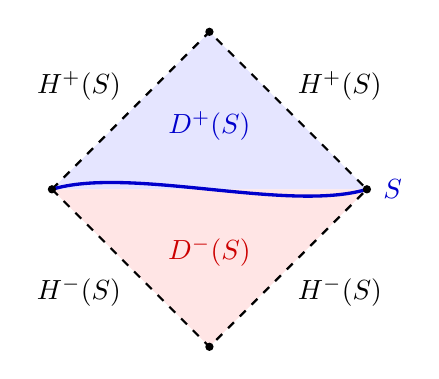
\begin{tikzpicture}[scale=1]
  % D+(S) Region
  \draw[thick, fill=blue!10, dashed] (-2,0) -- (0, 2) -- (2,0);
  % D-(S) Region
  \draw[thick, fill=red!10, dashed] (-2,0) -- (0, -2) -- (2,0);
  
  % Spacelike Surface S
  \draw[very thick, blue!80!black] (-2,0) .. controls (-1, 0.3) and (1, -0.3) .. (2,0) node[right=2pt] {$S$};
  
  % Labels
  \node[blue!80!black, font=\bfseries] at (0, 0.8) {$D^+(S)$};
  \node[red!80!black, font=\bfseries] at (0, -0.8) {$D^-(S)$};
  
  \node[above left] at (-1, 1) {$H^+(S)$};
  \node[above right] at (1, 1) {$H^+(S)$};
  
  \node[below left] at (-1, -1) {$H^-(S)$};
  \node[below right] at (1, -1) {$H^-(S)$};

  \fill (0,2) circle (1.5pt);
  \fill (0,-2) circle (1.5pt);
  \fill (-2,0) circle (1.5pt);
  \fill (2,0) circle (1.5pt);
\end{tikzpicture}
\end{center}


\subsection*{Failures of Causal Structure}

1. Poor Choice of Hypersurface: Slice not a Cauchy surface.
\begin{center}
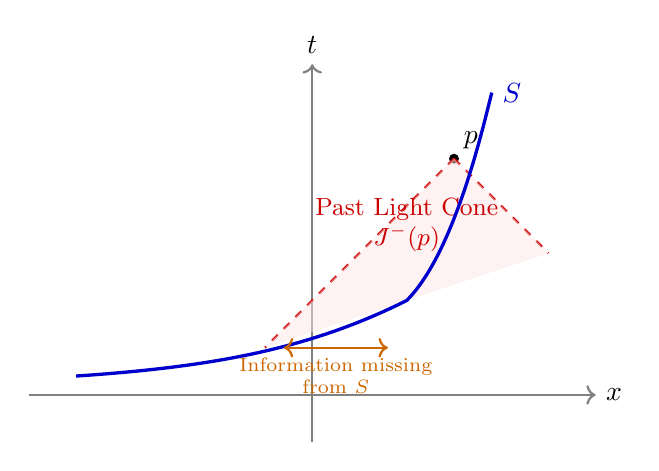
\begin{tikzpicture}[scale=1.2]
  % Axes
  \draw[->, thick, gray] (0,-0.5) -- (0, 3.5) node[above, text=black] {$t$};
  \draw[->, thick, gray] (-3,0) -- (3, 0) node[right, text=black] {$x$};
  
  % Point p
  \coordinate (P) at (1.5, 2.5);
  \fill[black] (P) circle (1.5pt) node[above right] {$p$};
  
  % Past Light Cone of p
  \draw[thick, red!80!black, dashed] (P) -- (-0.5, 0.5);
  \draw[thick, red!80!black, dashed] (P) -- (2.5, 1.5);
  \fill[red!10, opacity=0.5] (P) -- (-0.5, 0.5) -- (2.5, 1.5) -- cycle;
  \node[red!80!black, font=\small, align=center] at (1.0, 1.8) {Past Light Cone\\$J^-(p)$};

  % Hypersurface S (asymptotically approaching a null line, bounded)
  \draw[very thick, blue!80!black] (-2.5, 0.2) .. controls (-1, 0.3) and (0, 0.5) .. (1, 1) .. controls (1.5, 1.5) and (1.8, 2.8) .. (1.9, 3.2) node[right] {$S$};
  
  % Highlight intersection failure
  \draw[<->, thick, orange!80!black] (-0.3, 0.5) -- (0.8, 0.5) node[midway, below, font=\scriptsize, align=center] {Information missing\\from $S$};
\end{tikzpicture}
\end{center}



2. Closed Timelike Curves (CTCs): e.g., $R \times S^1$ metric:
\begin{equation} ds^2 = -\cos(\lambda) dt^2 - \sin(\lambda) (dt dx + dx dt) + \cos(\lambda) dx^2 \end{equation}
where $\lambda = \cot^{-1}(t)$. Light cones tilt, allowing CTCs.
\begin{center}
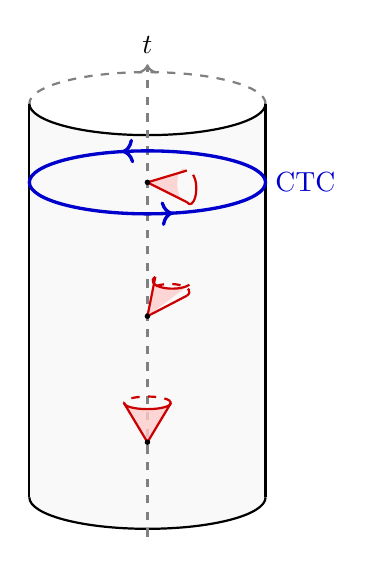
\begin{tikzpicture}[scale=1]
  % Cylinder background (back half)
  \draw[thick, dashed, gray] (1.5, 2.5) arc (0:180:1.5 and 0.4);
  \draw[thick, dashed, gray] (1.5, -2.5) arc (0:180:1.5 and 0.4);
  
  % Cylinder fill
  \path[fill=gray!5] (-1.5,-2.5) -- (-1.5,2.5) arc (180:360:1.5 and 0.4) -- (1.5,-2.5) arc (360:180:1.5 and 0.4) -- cycle;
  
  % Cylinder foreground
  \draw[thick] (-1.5, -2.5) -- (-1.5, 2.5);
  \draw[thick] (1.5, -2.5) -- (1.5, 2.5);
  \draw[thick] (-1.5, 2.5) arc (180:360:1.5 and 0.4);
  \draw[thick] (-1.5, -2.5) arc (180:360:1.5 and 0.4);

  % Axis
  \draw[->, thick, gray, dashed] (0, -3) -- (0, 3) node[above, text=black] {$t$};

  % Upright Light Cone (Bottom)
  \begin{scope}[shift={(0, -1.8)}]
    \fill[red!20, opacity=0.8] (0,0) -- (-0.3, 0.5) arc (180:360:0.3 and 0.08) -- cycle;
    \draw[thick, red!80!black] (0,0) -- (-0.3, 0.5);
    \draw[thick, red!80!black] (0,0) -- (0.3, 0.5);
    \draw[thick, red!80!black] (-0.3, 0.5) arc (180:360:0.3 and 0.08);
    \draw[thick, red!80!black, dashed] (0.3, 0.5) arc (0:180:0.3 and 0.08);
    \fill (0,0) circle (1pt);
  \end{scope}

  % Tilted Light Cone (Middle)
  \begin{scope}[shift={(0, -0.2)}]
    \fill[red!20, opacity=0.8] (0,0) -- (0.1, 0.5) arc (150:330:0.25 and 0.1) -- cycle;
    \draw[thick, red!80!black] (0,0) -- (0.1, 0.5);
    \draw[thick, red!80!black] (0,0) -- (0.5, 0.26);
    \draw[thick, red!80!black] (0.1, 0.5) arc (150:330:0.25 and 0.1);
    \draw[thick, red!80!black, dashed] (0.5, 0.26) arc (-30:150:0.25 and 0.1);
    \fill (0,0) circle (1pt);
  \end{scope}

  % Tipped Light Cone (Top - tangent to CTC)
  \begin{scope}[shift={(0, 1.5)}]
    \fill[red!20, opacity=0.8] (0,0) -- (0.5, 0.15) arc (60:240:0.08 and 0.2) -- cycle;
    \draw[thick, red!80!black] (0,0) -- (0.5, 0.15);
    \draw[thick, red!80!black] (0,0) -- (0.5, -0.25);
    \draw[thick, red!80!black] (0.5, -0.25) arc (240:420:0.08 and 0.2);
    \fill (0,0) circle (1pt);
  \end{scope}

  % Closed Timelike Curve (CTC) at t = 1.5
  \draw[very thick, blue!80!black, decoration={markings, mark=at position 0.3 with {\arrow{>}}, mark=at position 0.8 with {\arrow{>}}}, postaction={decorate}] (0, 1.5) ellipse (1.5 and 0.4);
  \node[blue!80!black, right] at (1.5, 1.5) {CTC};

\end{tikzpicture}
\end{center}



3. Singularities: Create Cauchy horizons where paths hit an "edge".
\begin{center}
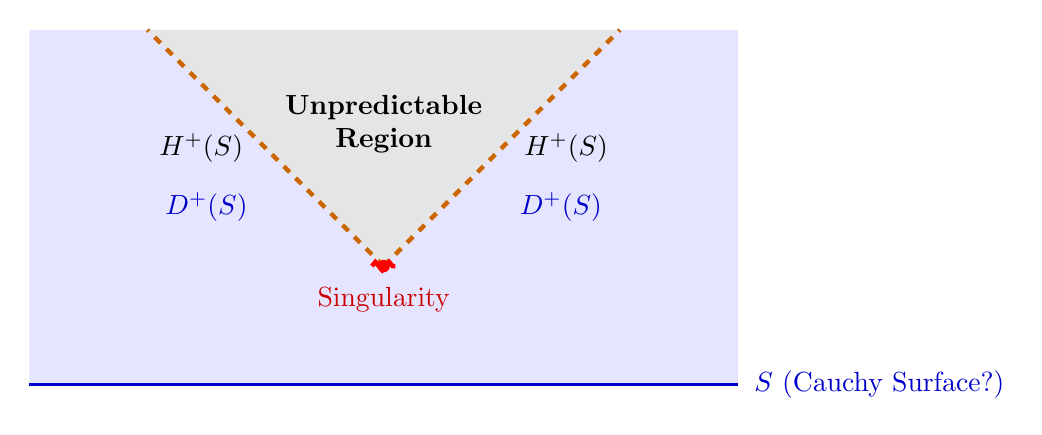
\begin{tikzpicture}[scale=1.5]
  % Future Light Cone of the Singularity (Unpredictable Region)
  \fill[gray!20] (0, 1) -- (-2, 3) -- (2, 3) -- cycle;
  
  % Domain of Dependence D+(S)
  \fill[blue!10] (-3, 0) -- (-3, 3) -- (-2, 3) -- (0, 1) -- (2, 3) -- (3, 3) -- (3, 0) -- cycle;

  % Cauchy Horizon H+(S)
  \draw[ultra thick, dashed, orange!80!black] (0, 1) -- (-2, 3) node[midway, left=4pt, text=black] {$H^+(S)$};
  \draw[ultra thick, dashed, orange!80!black] (0, 1) -- (2, 3) node[midway, right=4pt, text=black] {$H^+(S)$};

  % Singularity
  \draw[ultra thick, decorate, decoration={zigzag, segment length=5pt, amplitude=1.5pt}, red] (-0.1, 1) -- (0.1, 1);
  \fill[red] (0,1) circle (1.5pt);
  \node[red!80!black, below] at (0, 0.9) {Singularity};

  % Spacelike Surface S
  \draw[very thick, blue!80!black] (-3, 0) -- (3, 0) node[right=2pt] {$S$ (Cauchy Surface?)};

  % Labels
  \node[blue!80!black, font=\bfseries] at (-1.5, 1.5) {$D^+(S)$};
  \node[blue!80!black, font=\bfseries] at (1.5, 1.5) {$D^+(S)$};
  
  \node[font=\bfseries, align=center] at (0, 2.2) {Unpredictable\\Region};
  
\end{tikzpicture}
\end{center}


\section{Tensor Densities}
Densities transform with Jacobian determinant $|J|^W$.

\subsection*{The Levi-Civita Symbol}
$\tilde{\epsilon}_{\mu_1\mu_2\dots\mu_n}$ is $\pm 1$ or 0.


$$ \tilde{\epsilon}_{\mu'_1 \dots \mu'_n} |J|^{-1} = \tilde{\epsilon}_{\mu_1 \dots \mu_n} \frac{\partial x^{\mu_1}}{\partial x^{\mu'_1}} \dots \frac{\partial x^{\mu_n}}{\partial x^{\mu'_n}} $$


\begin{equation} \tilde{\epsilon}_{\mu'_1 \dots \mu'*n} = |J| \left( \tilde{\epsilon}*{\mu_1 \dots \mu_n} \frac{\partial x^{\mu_1}}{\partial x^{\mu'_1}} \dots \frac{\partial x^{\mu_n}}{\partial x^{\mu'_n}} \right) \end{equation}
Weight $W=+1$.

\subsection*{Determinant of the Metric}
$g' = \det(A^T g A) = (\det(A))^2 g$
\begin{equation} g' = (|J|^{-1})^2 g \implies g' = |J|^{-2} g \end{equation}
Weight $W=-2$.

\subsection*{The Levi-Civita Tensor}
Absorb $\sqrt{|g|}$ ($W=-1$) to make a true tensor ($W=0$):
\begin{equation} \epsilon_{\mu_1\mu_2\dots\mu_n} = \sqrt{|g|} \tilde{\epsilon}*{\mu_1\mu_2\dots\mu_n} \end{equation}
Contravariant tensor:
\begin{align*}
\epsilon^{\mu_1\dots\mu_n} &= \sqrt{|g|} \ g^{\alpha_1 \mu_1}\dots g^{\alpha_n \mu_n} \ \tilde{\epsilon}*{\alpha_1\dots\alpha_n} = \sqrt{|g|} \ |g|^{-1} \ \tilde{\epsilon}^{\mu_1\dots\mu_n}
\end{align*}
\begin{equation} \epsilon^{\mu_1\mu_2\dots\mu_n} = \frac{1}{\sqrt{|g|}} \tilde{\epsilon}^{\mu_1\mu_2\dots\mu_n} \end{equation}

\subsection*{Contraction Identity}
\begin{equation} \epsilon^{\mu_1\dots\mu_n} \epsilon_{\nu_1\dots\nu_n} = (-1)^s , \tilde{\epsilon}^{\mu_1\dots\mu_n} \tilde{\epsilon}*{\nu_1\dots\nu_n} \end{equation}
\begin{equation} \tilde{\epsilon}^{\mu_1\dots\mu_n} \tilde{\epsilon}*{\nu_1\dots\nu_n} = \delta^{\mu_1\dots\mu_n}*{\nu_1\dots\nu_n} = n! , \delta^{[\mu_1}*{\nu_1} \dots \delta^{\mu_n]}*{\nu_n} \end{equation}
Contracting $p$ indices:
\begin{equation} \delta^{\mu_1\dots\mu_p \alpha_1 \dots \alpha*{n-p}}*{\mu_1\dots\mu_p \beta_1 \dots \beta*{n-p}} = p! , \delta^{\alpha_1 \dots \alpha_{n-p}}*{\beta_1 \dots \beta*{n-p}} = p!(n-p)! , \delta^{[\alpha_1}*{\beta_1} \dots \delta^{\alpha*{n-p}]}*{\beta*{n-p}} \end{equation}
\begin{equation} \epsilon^{\mu_1\dots\mu_p\alpha_1\dots} \epsilon_{\mu_1\dots\mu_p\beta_1\dots} = (-1)^s p!(n-p)! \delta^{[\alpha_1}*{\beta_1} \dots \delta^{\alpha*{n-p}]}*{\beta*{n-p}} \end{equation}
Most common case ($p=n-1$):
\begin{equation} \epsilon^{\mu_1\dots\mu_{n-1}\alpha} \epsilon_{\mu_1\dots\mu_{n-1}\beta} = (-1)^s (n-1)! \delta^\alpha_\beta \end{equation}

\section{Differential Forms}
A $p$-form is a totally antisymmetric (0, $p$) tensor. Dimension $\binom{n}{p}$.

\subsection*{The Wedge Product}
\begin{equation} (A \wedge B)*{\mu_1 \dots \mu*{p+q}} = \frac{(p+q)!}{p!q!} A_{[\mu_1 \dots \mu_p} B_{\mu_{p+1} \dots \mu_{p+q}]} \end{equation}
\begin{equation} A \wedge B = (-1)^{pq} B \wedge A \end{equation}

\subsection*{The Exterior Derivative}
$d$ turns a $p$-form into a $(p+1)$-form:
\begin{equation} (dA)*{\mu_1 \dots \mu*{p+1}} = (p+1) \partial_{[\mu_1} A_{\mu_2 \dots \mu_{p+1}]} \end{equation}
Graded Leibniz Rule:
\begin{equation} d(A \wedge B) = (dA) \wedge B + (-1)^p A \wedge (dB) \end{equation}
$dA$ is a tensor because the non-tensorial part is symmetric and cancels under antisymmetrization:
\begin{align*}
(dA)*{\mu'\nu'} &= \partial*{\mu'} A_{\nu'} - \partial_{\nu'} A_{\mu'} \\
\text{Bad part} &= W_\nu \frac{\partial^2 x^\nu}{\partial x^{\mu'} \partial x^{\nu'}} - W_\nu \frac{\partial^2 x^\nu}{\partial x^{\mu'} \partial x^{\nu'}} = 0
\end{align*}


$d^2=0$ (exact forms are closed):
\begin{equation} d(dA) = 0 \end{equation}

\subsection*{The Double Dual Identity}
\begin{equation} \star\star A = (-1)^{s + p(n-p)} A \end{equation}
\begin{align*}
(\star\star A)*{\rho} &= \frac{1}{(n-p)!} \epsilon^{\sigma \dots}*{\rho \dots} \left( \frac{1}{p!} \epsilon^{\nu \dots}*{\sigma \dots} A*{\nu \dots} \right)
\end{align*}

\subsection*{Maxwell's Equations}
Faraday 2-form: \begin{equation} F = dA \end{equation}
Homogeneous: \begin{equation} dF = d(dA) = 0 \end{equation}
Inhomogeneous: \begin{equation} d(\star F) = \star J \end{equation}
Tensor form: $\star d \star F = \star \star J = J \implies \nabla_\mu F^{\mu\nu} = J^\nu$.
\begin{equation} \nabla_\mu F^{\mu\nu} = J^\nu \end{equation}

\section{Integration}
Volume element transforms as density $W=+1$:
\begin{equation} d^n x' = \left| \frac{\partial x^{\mu'}}{\partial x^\mu} \right| d^n x = |J| d^n x \end{equation}
Integration maps an $n$-form $\omega$ to $\mathbb{R}$:
\begin{equation} \int_\Sigma : \omega \to \mathbb{R} \end{equation}


\begin{center}
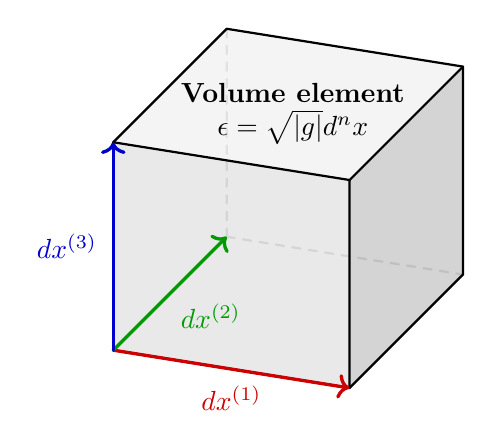
\begin{tikzpicture}[scale=1.2, line join=round, line cap=round]
  % Define origin and basis vectors
  \coordinate (O) at (0,0);
  \coordinate (V1) at (2.5, -0.4);
  \coordinate (V2) at (1.2, 1.2);
  \coordinate (V3) at (0, 2.2);

  % Calculate vertices
  \coordinate (V12) at ($(V1)+(V2)$);
  \coordinate (V13) at ($(V1)+(V3)$);
  \coordinate (V23) at ($(V2)+(V3)$);
  \coordinate (V123) at ($(V1)+(V2)+(V3)$);

  % Draw hidden (back) edges
  \draw[thick, dashed, gray] (O) -- (V2);
  \draw[thick, dashed, gray] (V2) -- (V12);
  \draw[thick, dashed, gray] (V2) -- (V23);

  % Fill visible faces with varying opacity for 3D effect
  \fill[gray!20, opacity=0.85] (O) -- (V1) -- (V13) -- (V3) -- cycle; % Front
  \fill[gray!40, opacity=0.85] (V1) -- (V12) -- (V123) -- (V13) -- cycle; % Right
  \fill[gray!10, opacity=0.85] (V3) -- (V13) -- (V123) -- (V23) -- cycle; % Top

  % Draw visible edges
  \draw[thick] (O) -- (V1) -- (V12) -- (V123) -- (V23) -- (V3) -- cycle;
  \draw[thick] (V1) -- (V13) -- (V3);
  \draw[thick] (V13) -- (V123);

  % Draw the three primary vectors
  \draw[->, very thick, red!80!black] (O) -- (V1) node[midway, below=2pt] {$dx^{(1)}$};
  \draw[->, very thick, green!60!black] (O) -- (V2) node[midway, below right] {$dx^{(2)}$};
  \draw[->, very thick, blue!80!black] (O) -- (V3) node[midway, left=2pt] {$dx^{(3)}$};

  % Label the volume
\node[font=\bfseries, align=center] at (1.9, 2.5) {Volume element \\ $\epsilon = \sqrt{|g|} d^n x$};
\end{tikzpicture}
\end{center}




\subsection*{The Invariant Volume Element}
Combining $\sqrt{|g|}$ ($W=-1$) and $d^n x$ ($W=+1$) yields invariant $n$-form.


$$ \epsilon = \frac{1}{n!} \sqrt{|g|} \tilde{\epsilon}_{\mu_1 \dots \mu_n} dx^{\mu_1} \wedge \dots \wedge dx^{\mu_n} $$


Using $\frac{1}{n!} \tilde{\epsilon}_{\mu_1 \dots \mu_n} dx^{\mu_1} \wedge \dots \wedge dx^{\mu_n} = d^n x$:
\begin{equation} \epsilon = \sqrt{|g|} d^n x \end{equation}
Invariant integral:
\begin{equation} S = \int \phi(x) \sqrt{|g|} d^n x \end{equation}
\begin{equation} S = \int \phi(x) \epsilon \end{equation}


\chapter{Curvature}

\section{Overview}
Curvature measures deviations from flat space, formalized by the Riemann tensor. This is built via a hierarchy of structures.

\textbf{1. The Connection (Christoffel Symbols):} Connects tangent spaces at different points.
\begin{equation}\label{eq:christoffel_preview}
\Gamma_{\mu\nu}^{\lambda} = \frac{1}{2}g^{\lambda\sigma} (\partial_{\mu}g_{\nu\sigma} + \partial_{\nu}g_{\sigma\mu} - \partial_{\sigma}g_{\mu\nu}).
\end{equation}
\textbf{2. The Covariant Derivative:} Upgrades partial derivatives to transform as tensors.
\begin{equation}\label{eq:cov_deriv_preview}
\nabla_{\mu}V^{\nu} = \partial_{\mu}V^{\nu} + \Gamma_{\mu\sigma}^{\nu}V^{\sigma}.
\end{equation}
\textbf{3. Geodesics:} Paths of zero acceleration in curved spacetime.
\begin{equation}\label{eq:geodesic_preview}
\frac{d^{2}x^{\mu}}{d\lambda^{2}} + \Gamma_{\rho\sigma}^{\mu} \frac{dx^{\rho}}{d\lambda} \frac{dx^{\sigma}}{d\lambda} = 0.
\end{equation}
\textbf{4. The Riemann Curvature Tensor:} The definitive measure of true curvature.
\begin{equation}\label{eq:riemann_preview}
{R^{\rho}}*{\sigma\mu\nu} = \partial*{\mu}\Gamma_{\nu\sigma}^{\rho} - \partial_{\nu}\Gamma_{\mu\sigma}^{\rho} + \Gamma_{\mu\lambda}^{\rho}\Gamma_{\nu\sigma}^{\lambda} - \Gamma_{\nu\lambda}^{\rho}\Gamma_{\mu\sigma}^{\lambda}.
\end{equation}

\section{Covariant Derivatives}
Partial derivatives of tensors fail to transform properly due to coordinate grid curvature:
\begin{equation}
V^{\nu'} = \frac{\partial x^{\nu'}}{\partial x^\nu} V^\nu.
\end{equation}
\begin{equation}
\partial_{\mu'} V^{\nu'} = \underbrace{\frac{\partial x^\mu}{\partial x^{\mu'}} \frac{\partial x^{\nu'}}{\partial x^\nu} (\partial_\mu V^\nu)}*{\text{Tensor part}} + \underbrace{\frac{\partial x^\mu}{\partial x^{\mu'}} \frac{\partial^2 x^{\nu'}}{\partial x^\mu \partial x^\nu} V^\nu}*{\text{Non-tensorial part}}.
\end{equation}

\subsection*{Defining the Covariant Derivative}
The covariant derivative $\nabla_\mu$ corrects this by incorporating the connection $\Gamma$:
\begin{equation}\label{eq:cov_deriv_vector}
\nabla_\mu V^\nu = \partial_\mu V^\nu + \Gamma^\nu_{\mu\lambda} V^\lambda.
\end{equation}
Requiring $\nabla_{\mu'} V^{\nu'} = \frac{\partial x^\mu}{\partial x^{\mu'}} \frac{\partial x^{\nu'}}{\partial x^\nu} \nabla_\mu V^\nu$ enforces the transformation law for $\Gamma$:
\begin{equation}\label{eq:gamma_transformation}
\Gamma^{\nu'}*{\mu'\lambda'} = \frac{\partial x^\mu}{\partial x^{\mu'}} \frac{\partial x^\lambda}{\partial x^{\lambda'}} \frac{\partial x^{\nu'}}{\partial x^\nu} \Gamma^\nu*{\mu\lambda} - \frac{\partial x^\mu}{\partial x^{\mu'}} \frac{\partial x^{\lambda}}{\partial x^{\lambda'}} \frac{\partial^2 x^{\nu'}}{\partial x^\mu \partial x^\lambda}.
\end{equation}

For a one-form $\omega_\lambda$, preserving the Leibniz rule yields a negative connection term:
\begin{equation}
\nabla_\mu \omega_\lambda = \partial_\mu \omega_\lambda - \Gamma^\sigma_{\mu\lambda} \omega_\sigma.
\end{equation}

\subsection*{The Christoffel Connection}
General relativity relies on the unique metric-compatible ($\nabla_\rho g_{\mu\nu} = 0$) and torsion-free ($\Gamma^\lambda_{\mu\nu} = \Gamma^\lambda_{\nu\mu}$) connection.

\textbf{1. Covariant Derivative of the Inverse Metric:}
\begin{equation}
\nabla_\rho (g^{\mu\sigma} g_{\sigma\nu}) = 0 \implies (\nabla_\rho g^{\mu\sigma}) g_{\sigma\nu} = 0 \implies \nabla_\rho g^{\mu\lambda} = 0.
\end{equation}
\textbf{2. Covariant Derivative of the Levi-Civita Tensor:}
In locally inertial coordinates ($\Gamma = 0, \partial g = 0$), $\partial_\lambda g = 0 \implies \partial_\lambda \sqrt{|g|} = 0$.
\begin{equation}
\nabla_\lambda \epsilon_{\mu\nu\rho\sigma} = \partial_\lambda (\sqrt{|g|} \tilde{\epsilon}_{\mu\nu\rho\sigma}) = 0.
\end{equation}

Permuting metric compatibility $\nabla_\rho g_{\mu\nu} = 0$ yields the Christoffel formula:
\begin{equation}\label{eq:christoffel_formula}
\Gamma^\sigma_{\mu\nu} = \frac{1}{2} g^{\sigma\rho} ( \partial_\mu g_{\nu\rho} + \partial_\nu g_{\rho\mu} - \partial_\rho g_{\mu\nu} ).
\end{equation}

\subsection*{Divergence Formula}
Contracting indices on the Christoffel symbol provides an identity for the metric determinant $g$:
\begin{equation}\label{eq:gamma_contracted}
\Gamma^\mu_{\mu\lambda} = \frac{1}{2} g^{\mu\nu} \partial_\lambda g_{\mu\nu} = \frac{1}{2} \left( \frac{1}{g} \partial_\lambda g \right) = \frac{1}{\sqrt{|g|}} \partial_\lambda \sqrt{|g|}.
\end{equation}
This leads to the divergence formula and Stokes' theorem in curved space:
\begin{equation}
\nabla_\mu V^\mu = \frac{1}{\sqrt{|g|}} \partial_\mu (\sqrt{|g|} V^\mu)
\end{equation}
\begin{equation}
\int_{\mathcal{V}} d^n x \sqrt{|g|} \nabla_\mu V^\mu = \int_{\partial \mathcal{V}} d^{n-1} x \sqrt{|\gamma|} n_\mu V^\mu
\end{equation}

\section{Parallel Transport and Geodesics}


\begin{center}
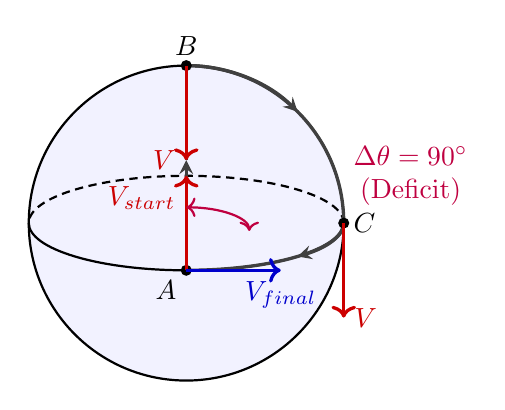
\begin{tikzpicture}[scale=2]
  % Sphere Base
  \draw[thick, fill=blue!5] (0,0) circle (1);
  
  % Equator
  \draw[thick, densely dashed] (1,0) arc (0:180:1 and 0.3);
  \draw[thick] (-1,0) arc (180:360:1 and 0.3);

  % Geodesic Paths
  % Path A -> B (Central Meridian)
  \draw[very thick, darkgray, -stealth] (0,-0.3) -- (0, 0.4);
  \draw[very thick, darkgray] (0,0.4) -- (0,1);
  
  % Path B -> C (Right Meridian)
  \draw[very thick, darkgray, -stealth] (0,1) arc (90:45:1 and 1);
  \draw[very thick, darkgray] (0,1) arc (90:0:1 and 1);
  
  % Path C -> A (Equator segment)
  \draw[very thick, darkgray, -stealth] (1,0) arc (360:315:1 and 0.3);
  \draw[very thick, darkgray] (1,0) arc (360:270:1 and 0.3);

  % Key Points
  \fill (0,-0.3) circle (1pt) node[below left] {$A$};
  \fill (0,1) circle (1pt) node[above] {$B$};
  \fill (1,0) circle (1pt) node[right] {$C$};

  % Transported Vectors
  % Initial Vector at A (Pointing North)
  \draw[->, very thick, red!80!black] (0,-0.3) -- (0, 0.3) node[below left] {$V_{start}$};
  
  % Vector transported to B (Points South along central meridian)
  \draw[->, very thick, red!80!black] (0,1) -- (0, 0.4) node[left] {$V$};
  
  % Vector transported to C (Maintains angle with meridian, points South)
  \draw[->, very thick, red!80!black] (1,0) -- (1, -0.6) node[right] {$V$};
  
  % Vector returned to A (Parallel to equator, points East)
  \draw[->, very thick, blue!80!black] (0,-0.3) -- (0.6, -0.3) node[below] {$V_{final}$};

  % Highlight Deficit Angle at A
  \draw[<->, thick, purple] (0, 0.1) arc (90:0:0.4 and 0.15);
  \node[purple, right, align=center] at (1, 0.3) {$\Delta\theta = 90^\circ$ \\ (Deficit)};
\end{tikzpicture}
\end{center}



A vector $V^\mu$ is parallel transported along $x^\mu(\lambda)$ if its directional covariant derivative vanishes:
\begin{equation}\label{eq:parallel_transport}
\frac{D V^\mu}{d\lambda} \equiv \frac{dx^\nu}{d\lambda} \nabla_\nu V^\mu = 0 \implies \frac{d V^\mu}{d\lambda} + \Gamma^\mu_{\sigma\rho} \frac{dx^\sigma}{d\lambda} V^\rho = 0.
\end{equation}

\subsection*{Geodesic Equation}
A geodesic parallel transports its own tangent vector $U^\mu = dx^\mu/d\lambda$:
\begin{equation}\label{eq:geodesic_eq}
\frac{d^2 x^\mu}{d\lambda^2} + \Gamma^\mu_{\rho\sigma} \frac{dx^\rho}{d\lambda} \frac{dx^\sigma}{d\lambda} = 0.
\end{equation}

\subsection*{Variational Principle}
Geodesics also extremize the energy integral $I = \frac{1}{2} \int g_{\mu\nu} \dot{x}^\mu \dot{x}^\nu d\tau$. Varying $\delta I = 0$ yields:
\begin{equation}
g_{\sigma\nu} \ddot{x}^\nu + \frac{1}{2} \left( \partial_\mu g_{\sigma\nu} + \partial_\nu g_{\sigma\mu} - \partial_\sigma g_{\mu\nu} \right) \dot{x}^\mu \dot{x}^\nu = 0.
\end{equation}
Multiplying by $g^{\lambda\sigma}$ recovers the geodesic equation exactly.

\subsection*{Null Geodesics}
Massless particles follow null geodesics ($ds^2 = 0$) parameterized by affine parameter $\lambda$ such that $p^\mu = dx^\mu/d\lambda$:
\begin{equation}
p^\nu \nabla_\nu p^\mu = 0.
\end{equation}
Observed energy is $E = - p_\mu U^\mu_{\text{obs}}$.

\section{Properties of Geodesics}

\subsection*{Affine Parameters}
Affine parameters $\lambda$ are unique up to linear transformations $\alpha = a\lambda + b$. Under an arbitrary parameter change $\alpha(\lambda)$:
\begin{equation}
\left( \frac{d\alpha}{d\lambda} \right)^2 \left[ \frac{d^2 x^\mu}{d\alpha^2} + \Gamma^\mu_{\rho\sigma} \frac{dx^\rho}{d\alpha} \frac{dx^\sigma}{d\alpha} \right] + \frac{dx^\mu}{d\alpha} \frac{d^2\alpha}{d\lambda^2} = 0.
\end{equation}
For $\alpha$ to be affine, $d^2\alpha/d\lambda^2 = 0$.

\subsection*{Riemann Normal Coordinates (RNC)}
The exponential map allows construction of RNC $x^{\hat{\mu}}(q) = k^{\hat{\mu}}$, where geodesics from $p$ are straight lines $x^{\hat{\mu}}(\lambda) = \lambda k^{\hat{\mu}}$. At $p$:
\begin{equation}
\Gamma^{\hat{\mu}}*{\hat{\rho}\hat{\sigma}}(p) = 0 \implies \partial*{\hat{\rho}} g_{\hat{\mu}\hat{\nu}}(p) = 0.
\end{equation}

\section{The Expanding Universe Revisited}
Robertson-Walker metric ($k=0$):
\begin{equation}
ds^2 = -dt^2 + a^2(t) \delta_{ij} dx^i dx^j.
\end{equation}
Varying $I = \frac{1}{2} \int \left[ -(\dot{t})^2 + a^2(t) \delta_{ij} \dot{x}^i \dot{x}^j \right] d\tau$ gives connection coefficients:
\begin{align}
\Gamma^0_{00} &= 0, \quad \Gamma^0_{0i} = 0, \quad \Gamma^0_{ij} = a\dot{a} \delta_{ij}, \\
\Gamma^k_{0j} &= \frac{\dot{a}}{a} \delta^k_j, \quad \Gamma^k_{ij} = 0, \quad \Gamma^k_{00} = 0.
\end{align}

\subsection*{Cosmological Redshift}
For a null geodesic $\frac{dx}{dt} = \frac{1}{a(t)}$, the $t$-equation implies:
\begin{equation}
\frac{d}{d\lambda} \ln \left( \frac{dt}{d\lambda} \right) = - \frac{d}{d\lambda} \ln a \implies \frac{dt}{d\lambda} = \frac{\omega_0}{a(t)}.
\end{equation}
Energy $E = -p_\mu U^\mu \propto 1/a(t)$.

\subsection*{Conservation of Energy-Momentum}
For perfect fluid $T^{\mu\nu} = (\rho + p)U^\mu U^\nu + p g^{\mu\nu}$, $\nabla_\mu T^{\mu 0} = 0$ implies:
\begin{equation}
\dot{\rho} + 3\frac{\dot{a}}{a} (\rho + p) = 0.
\end{equation}
Given $p=w\rho$, $\rho \propto a^{-3(1+w)}$.

\section{The Riemann Curvature Tensor}


\begin{center}
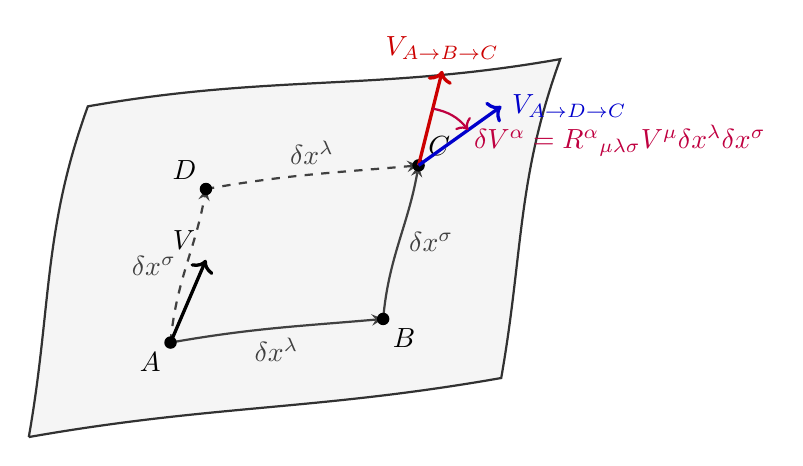
\begin{tikzpicture}[scale=1.5]
  % Curved surface patch
  \draw[thick, fill=gray!10, opacity=0.8] (0,0) to[out=10, in=190] (4,0.5) 
        to[out=80, in=250] (4.5,3.2) 
        to[out=190, in=10] (0.5,2.8) 
        to[out=250, in=80] (0,0);

  % Loop Coordinates
  \coordinate (A) at (1.2, 0.8);
  \coordinate (B) at (3.0, 1.0);
  \coordinate (C) at (3.3, 2.3);
  \coordinate (D) at (1.5, 2.1);

  % Loop Paths (A->B->C and A->D->C)
  \draw[thick, darkgray, -stealth] (A) to[out=10, in=185] node[midway, below] {$\delta x^\lambda$} (B);
  \draw[thick, darkgray, -stealth] (B) to[out=85, in=260] node[midway, right] {$\delta x^\sigma$} (C);
  \draw[thick, darkgray, dashed, -stealth] (A) to[out=85, in=260] node[midway, left] {$\delta x^\sigma$} (D);
  \draw[thick, darkgray, dashed, -stealth] (D) to[out=10, in=185] node[midway, above] {$\delta x^\lambda$} (C);

  % Vertices
  \fill (A) circle (1.5pt) node[below left] {$A$};
  \fill (B) circle (1.5pt) node[below right] {$B$};
  \fill (C) circle (1.5pt) node[above right] {$C$};
  \fill (D) circle (1.5pt) node[above left] {$D$};

  % Initial Vector at A
  \draw[->, very thick, black] (A) -- ++(0.3, 0.7) node[above left] {$V$};

  % Transported Vectors at C
  \coordinate (V1) at ($(C) + (0.2, 0.8)$); % Transported via B
  \coordinate (V2) at ($(C) + (0.7, 0.5)$); % Transported via D

  \draw[->, very thick, red!80!black] (C) -- (V1) node[above] {$V_{A \to B \to C}$};
  \draw[->, very thick, blue!80!black] (C) -- (V2) node[right] {$V_{A \to D \to C}$};

  % Riemann Curvature Deficit Vector
  \draw[->, thick, purple] ($(C)!0.6!(V1)$) to[bend left=20] node[below=9pt, right=4pt] {$\delta V^\alpha = R^\alpha{}_{\mu\lambda\sigma} V^\mu \delta x^\lambda \delta x^\sigma$} ($(C)!0.6!(V2)$);
\end{tikzpicture}
\end{center}


The commutator of covariant derivatives acting on vector $V^\rho$ reveals curvature:
\begin{equation}
[\nabla_\mu, \nabla_\nu] V^\rho = \left( \partial_\mu \Gamma^\rho_{\nu\sigma} - \partial_\nu \Gamma^\rho_{\mu\sigma} + \Gamma^\rho_{\mu\lambda} \Gamma^\lambda_{\nu\sigma} - \Gamma^\rho_{\nu\lambda} \Gamma^\lambda_{\mu\sigma} \right) V^\sigma - 2\Gamma^\lambda_{[\mu\nu]} \nabla_\lambda V^\rho.
\end{equation}
For a torsion-free connection, this defines the Riemann tensor ${R^\rho}_{\sigma\mu\nu}$:
\begin{equation}\label{eq:riemann_def}
[\nabla_\mu, \nabla_\nu] V^\rho = {R^\rho}*{\sigma\mu\nu} V^\sigma.
\end{equation}
Change in $V^\alpha$ around a small loop $\delta x^\lambda, \delta x^\sigma$:
\begin{equation}
\delta V^{\alpha} = {R^{\alpha}}*{\mu\lambda\sigma} V^{\mu} \delta x^{\lambda} \delta x^{\sigma}.
\end{equation}

\subsection*{Theorem: Flatness}
$R^\rho{}_{\sigma\mu\nu} = 0$ everywhere if and only if there exists a coordinate system where $\partial_\sigma g_{\mu\nu} = 0$ everywhere.
Proof involves defining a parallel-transported dual basis $\nabla_\mu \omega_\nu = 0$, implying $d\omega = 0 \implies \omega_a = dy^a$, yielding constant metric $ds^2 = \eta_{ab} dy^a dy^b$.

\section{Properties of the Riemann Tensor}
\subsection*{Symmetries}
Evaluated in RNC, $R_{\rho\sigma\mu\nu} = \frac{1}{2} (\partial_\mu \partial_\sigma g_{\rho\nu} - \partial_\mu \partial_\rho g_{\nu\sigma} - \partial_\nu \partial_\sigma g_{\rho\mu} + \partial_\nu \partial_\rho g_{\mu\sigma})$ yields:
\begin{align}
R_{\rho\sigma\mu\nu} &= -R_{\sigma\rho\mu\nu} \quad (\text{Antisymmetry first pair}) \\
R_{\rho\sigma\mu\nu} &= -R_{\rho\sigma\nu\mu} \quad (\text{Antisymmetry last pair}) \\
R_{\rho\sigma\mu\nu} &= R_{\mu\nu\rho\sigma} \quad (\text{Symmetry pair exchange}) \\
R_{\rho[\sigma\mu\nu]} &= 0 \quad (\text{First Bianchi Identity})
\end{align}
These reduce independent components to $\frac{1}{12}n^2(n^2 - 1)$ (20 components in 4D).

\subsection*{Second Bianchi Identity}
Differentiating $R$ in RNC gives the differential identity:
\begin{equation}
\nabla_{[\lambda} R_{\rho\sigma]\mu\nu} = 0.
\end{equation}

\subsection*{Ricci, Einstein, and Weyl Tensors}
\textbf{Ricci Tensor / Scalar:}
\begin{equation}
R_{\mu\nu} = {R^\lambda}*{\mu\lambda\nu}, \quad R = g^{\mu\nu} R*{\mu\nu}.
\end{equation}
\textbf{Einstein Tensor:}
Contracting the Second Bianchi Identity twice yields the divergence-free Einstein tensor:
\begin{equation}
\nabla^\mu \left( R_{\rho\mu} - \frac{1}{2} R g_{\rho\mu} \right) = 0 \implies G_{\mu\nu} = R_{\mu\nu} - \frac{1}{2} R g_{\mu\nu}, \quad \nabla^\mu G_{\mu\nu} = 0.
\end{equation}
\textbf{Weyl Tensor (Trace-Free):}
\begin{equation}
C_{\rho\sigma\mu\nu} = R_{\rho\sigma\mu\nu} - \frac{2}{n-2} (g_{\rho[\mu} R_{\nu]\sigma} - g_{\sigma[\mu} R_{\nu]\rho}) + \frac{2}{(n-1)(n-2)} g_{\rho[\mu} g_{\nu]\sigma} R.
\end{equation}

\section{Mathematical Interlude: Diffeomorphisms and Lie Derivatives}
The Lie Derivative $\mathcal{L}_V$ measures tensor change along vector field $V^\mu$ flow without a connection:
\begin{align}
\mathcal{L}*V U^\mu &= [V, U]^\mu = V^\nu \partial*\nu U^\mu - U^\nu \partial_\nu V^\mu \\
\mathcal{L}*V \omega*\mu &= V^\nu \partial_\nu \omega_\mu + \omega_\nu \partial_\mu V^\nu \\
\mathcal{L}*V {T^\mu}*\nu &= V^\lambda \nabla_\lambda {T^\mu}*\nu - (\nabla*\lambda V^\mu) {T^\lambda}*\nu + (\nabla*\nu V^\lambda) {T^\mu}_\lambda
\end{align}

\section{Symmetries and Killing Vectors}
A metric symmetry $\partial_{\sigma_*} g_{\mu\nu} = 0$ implies conserved momentum along geodesics $dp_{\sigma_*}/d\tau = 0$. For generator $K^\mu$, $K^\nu p_\nu$ is conserved.
\begin{equation}
\frac{d}{d\tau} (K_\nu p^\nu) = p^\mu p^\nu \nabla_{(\mu} K_{\nu)} = 0.
\end{equation}
This gives \textbf{Killing's Equation}:
\begin{equation}\label{eq:killing_eq}
\nabla_{(\mu} K_{\nu)} = \frac{1}{2} (\nabla_\mu K_\nu + \nabla_\nu K_\mu) = 0.
\end{equation}
Using the covariant derivative expansion, $\nabla_\mu K_\nu = \partial_\mu K_\nu - \Gamma^\lambda_{\mu\nu} K_\lambda$.



\chapter{Gravitation}

\section{Physics in Curved Spacetime}

In Newtonian gravity, body response and potential generation are governed by:
\begin{equation}
\label{eq:newton_accel}
\mathbf{a} = -\nabla\Phi \quad \implies \quad \frac{d^{2}x^{i}}{dt^{2}} = -\partial_{i}\Phi.
\end{equation}
\begin{equation}
\label{eq:poisson}
\nabla^{2}\Phi = 4\pi G\rho,
\end{equation}

\subsection*{The Minimal-Coupling Principle}
Based on the Einstein Equivalence Principle (EEP), laws generalize to curved spacetime via the minimal-coupling principle (Comma-Goes-to-Semicolon Rule: $\eta_{\mu\nu} \rightarrow g_{\mu\nu}$, $\partial_{\mu} \rightarrow \nabla_{\mu}$).

\subsection*{Derivation of the Geodesic Equation}
In flat spacetime, a free particle path $x^\mu(\lambda)$ obeys:
\begin{equation}
\label{eq:flat_motion}
\frac{d^{2}x^{\mu}}{d\lambda^{2}} = 0.
\end{equation}
Rewriting using the directional derivative:
\begin{equation}
\frac{d}{d\lambda} = \frac{dx^{\nu}}{d\lambda}\partial_{\nu}.
\end{equation}
\begin{equation}
\label{eq:flat_motion_chain}
\frac{dx^{\nu}}{d\lambda}\partial_{\nu}\left(\frac{dx^{\mu}}{d\lambda}\right) = 0.
\end{equation}
Applying minimal coupling ($\partial_{\nu} \rightarrow \nabla_{\nu}$):
\begin{equation}
\frac{dx^{\nu}}{d\lambda}\nabla_{\nu}\left(\frac{dx^{\mu}}{d\lambda}\right) = 0.
\end{equation}
Expanding the covariant derivative:
\begin{equation}
\nabla_{\nu} V^{\mu} = \partial_{\nu} V^{\mu} + \Gamma^{\mu}*{\nu\rho} V^{\rho}.
\end{equation}
Substituting back:
\begin{align}
\frac{dx^{\nu}}{d\lambda} \left[ \partial*{\nu}\left(\frac{dx^{\mu}}{d\lambda}\right) + \Gamma^{\mu}*{\nu\rho}\left(\frac{dx^{\rho}}{d\lambda}\right) \right] &= 0 \nonumber \\
\frac{dx^{\nu}}{d\lambda} \partial*{\nu}\left(\frac{dx^{\mu}}{d\lambda}\right) + \Gamma^{\mu}*{\nu\rho}\frac{dx^{\nu}}{d\lambda}\frac{dx^{\rho}}{d\lambda} &= 0.
\end{align}
Yielding the \textbf{geodesic equation}:
\begin{equation}
\label{eq:geodesic_derivation}
\frac{d^{2}x^{\mu}}{d\lambda^{2}} + \Gamma^{\mu}*{\rho\sigma}\frac{dx^{\rho}}{d\lambda}\frac{dx^{\sigma}}{d\lambda} = 0,
\end{equation}

\subsection*{Energy-Momentum Conservation}
Flat spacetime conservation $\partial_{\mu}T^{\mu\nu} = 0$ generalizes to:
\begin{equation}
\nabla_{\mu}T^{\mu\nu} = 0.
\end{equation}

\subsection*{The Newtonian Limit}
Requires: 1. Slow motion ($v \ll c$), 2. Static field ($\partial_{0} g_{\alpha\beta} = 0$), 3. Weak field ($g_{\mu\nu} = \eta_{\mu\nu} + h_{\mu\nu}$).

\subsubsection*{1. Simplifying the Geodesic Equation}
Slow motion implies:
\begin{equation}
\left| \frac{dx^{i}}{d\tau} \right| \ll \left| \frac{dt}{d\tau} \right|.
\end{equation}
Geodesic equation simplifies to:
\begin{equation}
\label{eq:geodesic_slow}
\frac{d^{2}x^{\mu}}{d\tau^{2}} + \Gamma^{\mu}_{00}\left(\frac{dt}{d\tau}\right)^{2} = 0.
\end{equation}

\subsubsection*{2. Evaluating the Christoffel Symbol}
\begin{equation}
\Gamma^{\mu}*{00} = \frac{1}{2}g^{\mu\lambda}(\partial*{0}g_{\lambda 0} + \partial_{0}g_{0\lambda} - \partial_{\lambda}g_{00}).
\end{equation}
Static field assumption gives:
\begin{equation}
\label{eq:gamma_00_static}
\Gamma^{\mu}*{00} = -\frac{1}{2}g^{\mu\lambda}\partial*{\lambda}g_{00}.
\end{equation}

\subsubsection*{3. The Weak Field Approximation}
\begin{equation}
g_{\mu\nu} = \eta_{\mu\nu} + h_{\mu\nu}, \quad |h_{\mu\nu}| \ll 1.
\end{equation}
Inverse metric to linear order $g^{\mu\nu} = \eta^{\mu\nu} - h^{\mu\nu}$:
\begin{align}
g^{\mu\lambda}g_{\lambda\nu} &= (\eta^{\mu\lambda} - h^{\mu\lambda})(\eta_{\lambda\nu} + h_{\lambda\nu}) \nonumber \\
&= \eta^{\mu\lambda}\eta_{\lambda\nu} + \eta^{\mu\lambda}h_{\lambda\nu} - h^{\mu\lambda}\eta_{\lambda\nu} - h^{\mu\lambda}h_{\lambda\nu} \nonumber \\
&= \delta^{\mu}*{\nu} + \eta^{\mu\lambda}h*{\lambda\nu} - (\eta^{\mu\rho}\eta^{\lambda\sigma}h_{\rho\sigma})\eta_{\lambda\nu} + \mathcal{O}(h^{2}) \nonumber \\
&= \delta^{\mu}*{\nu} + \eta^{\mu\lambda}h*{\lambda\nu} - \eta^{\mu\rho}\delta^{\sigma}*{\nu}h*{\rho\sigma} \nonumber \\
&= \delta^{\mu}*{\nu} + \eta^{\mu\lambda}h*{\lambda\nu} - \eta^{\mu\rho}h_{\rho\nu}.
\end{align}
Replacing inverse metric with flat metric:
\begin{equation}
\Gamma^{\mu}*{00} \approx -\frac{1}{2}\eta^{\mu\lambda}\partial*{\lambda}h_{00}.
\end{equation}
Substituting into \eqref{eq:geodesic_slow}:
\begin{equation}
\label{eq:geodesic_weak}
\frac{d^{2}x^{\mu}}{d\tau^{2}} = \frac{1}{2}\eta^{\mu\lambda}\partial_{\lambda}h_{00}\left(\frac{dt}{d\tau}\right)^{2}.
\end{equation}

\subsubsection*{4. Decomposing Time and Spatial Components}
Time Component ($\mu = 0$):
\begin{equation}
\frac{d^{2}t}{d\tau^{2}} = \frac{1}{2}\eta^{0\lambda}\partial_{\lambda}h_{00}\left(\frac{dt}{d\tau}\right)^{2} = \frac{1}{2}\eta^{00}\partial_{0}h_{00}\left(\frac{dt}{d\tau}\right)^{2}.
\end{equation}
Static field gives:
\begin{equation}
\frac{d^{2}t}{d\tau^{2}} = 0 \quad \implies \quad \frac{dt}{d\tau} = \text{constant}.
\end{equation}
Spatial Components ($\mu = i$):
\begin{equation}
\frac{d^{2}x^{i}}{d\tau^{2}} = \frac{1}{2}\eta^{ij}\partial_{j}h_{00}\left(\frac{dt}{d\tau}\right)^{2} = \frac{1}{2}\delta^{ij}\partial_{j}h_{00}\left(\frac{dt}{d\tau}\right)^{2} = \frac{1}{2}\partial_{i}h_{00}\left(\frac{dt}{d\tau}\right)^{2}.
\end{equation}
Applying chain rule:
\begin{equation}
\frac{d}{d\tau} = \frac{dt}{d\tau} \frac{d}{dt} \quad \implies \quad \frac{d^{2}x^{i}}{d\tau^{2}} = \frac{d}{d\tau}\left( \frac{dt}{d\tau}\frac{dx^{i}}{dt} \right).
\end{equation}
\begin{equation}
\frac{d^{2}x^{i}}{d\tau^{2}} = \left(\frac{d^{2}t}{d\tau^{2}}\right)\frac{dx^{i}}{dt} + \frac{dt}{d\tau} \frac{d}{d\tau}\left(\frac{dx^{i}}{dt}\right).
\end{equation}
\begin{equation}
\frac{d^{2}x^{i}}{d\tau^{2}} = \left(\frac{dt}{d\tau}\right)^{2} \frac{d^{2}x^{i}}{dt^{2}}.
\end{equation}
Substituting back:
\begin{equation}
\left(\frac{dt}{d\tau}\right)^{2} \frac{d^{2}x^{i}}{dt^{2}} = \frac{1}{2}\partial_{i}h_{00}\left(\frac{dt}{d\tau}\right)^{2} \quad \implies \quad \frac{d^{2}x^{i}}{dt^{2}} = \frac{1}{2}\partial_{i}h_{00}.
\end{equation}

\subsubsection*{5. Connection to the Newtonian Potential}
Equating to Newtonian acceleration \eqref{eq:newton_accel}:
\begin{equation}
\frac{d^{2}x^{i}}{dt^{2}} = \frac{1}{2}\partial_{i}h_{00} \quad \text{vs} \quad \frac{d^{2}x^{i}}{dt^{2}} = -\partial_{i}\Phi.
\end{equation}
\begin{equation}
\label{eq:h00_phi}
\frac{1}{2}\partial_{i}h_{00} = -\partial_{i}\Phi \quad \implies \quad h_{00} = -2\Phi.
\end{equation}
\begin{equation}
g_{00} = -(1 + 2\Phi).
\end{equation}

\section{Einstein's Equation}

\subsection{Motivating the Tensorial Equation}
Generalizing Poisson's equation:
\begin{equation}
\label{eq:poisson_equation}
\nabla^{2}\Phi = 4\pi G\rho,
\end{equation}
\begin{equation}
[\nabla^{2}g]*{\mu\nu} \propto T*{\mu\nu}.
\end{equation}
Naive guess:
\begin{equation}
\label{eq:naive_einstein}
R_{\mu\nu} = \kappa T_{\mu\nu},
\end{equation}

\subsection{The Conservation of Energy Problem}
Local energy conservation $\nabla^{\mu}T_{\mu\nu} = 0$ implies $\nabla^{\mu}R_{\mu\nu} = 0$.
However, the contracted Bianchi identity states:
\begin{equation}
\label{eq:contracted_bianchi_again}
\nabla^{\mu}R_{\mu\nu} = \frac{1}{2}\nabla_{\nu}R,
\end{equation}
\begin{equation}
g^{\mu\nu}R_{\mu\nu} = \kappa g^{\mu\nu}T_{\mu\nu} \quad \implies \quad R = \kappa T.
\end{equation}
\begin{equation}
\nabla^{\mu}R_{\mu\nu} = \frac{1}{2}\nabla_{\nu}(\kappa T).
\end{equation}
\begin{equation}
\frac{1}{2}\kappa \nabla_{\nu}T = 0 \quad \implies \quad \nabla_{\nu}T = 0.
\end{equation}

\subsection{The Einstein Tensor}
Rearranging the contracted Bianchi identity:
\begin{equation}
\nabla^{\mu}R_{\mu\nu} - \frac{1}{2}\nabla_{\nu}R = 0.
\end{equation}
\begin{equation}
\nabla^{\mu}R_{\mu\nu} - \frac{1}{2}g_{\mu\nu}\nabla^{\mu}R = 0 \quad \implies \quad \nabla^{\mu}\left( R_{\mu\nu} - \frac{1}{2}R g_{\mu\nu} \right) = 0.
\end{equation}
Defining the \textbf{Einstein Tensor}:
\begin{equation}
\label{eq:einstein_tensor_def}
G_{\mu\nu} \equiv R_{\mu\nu} - \frac{1}{2}R g_{\mu\nu}.
\end{equation}
Proposed field equation:
\begin{equation}
\label{eq:einstein_proposed}
G_{\mu\nu} = \kappa T_{\mu\nu}.
\end{equation}

\subsection{The Trace-Reversed Form}
Taking the trace in 4D:
\begin{align}
g^{\mu\nu} G_{\mu\nu} &= \kappa g^{\mu\nu} T_{\mu\nu} \nonumber \\
g^{\mu\nu} \left( R_{\mu\nu} - \frac{1}{2}R g_{\mu\nu} \right) &= \kappa T \nonumber \\
R - \frac{1}{2}R (g^{\mu\nu}g_{\mu\nu}) &= \kappa T.
\end{align}
\begin{equation}
R - \frac{1}{2}R(4) = \kappa T \quad \implies \quad R - 2R = \kappa T \quad \implies \quad R = -\kappa T.
\end{equation}
\begin{equation}
R_{\mu\nu} - \frac{1}{2}(-\kappa T)g_{\mu\nu} = \kappa T_{\mu\nu}.
\end{equation}
Yielding the \textbf{trace-reversed form}:
\begin{equation}
\label{eq:einstein_trace_reversed}
R_{\mu\nu} = \kappa \left( T_{\mu\nu} - \frac{1}{2}T g_{\mu\nu} \right).
\end{equation}

\subsection{The Newtonian Limit and the Coupling Constant}
For pressureless dust:
\begin{equation}
T_{\mu\nu} = \rho U_{\mu}U_{\nu}.
\end{equation}
Using weak-field metric $g_{00} = -1 + h_{00}$:
\begin{equation}
g_{00}(U^{0})^{2} = -1 \quad \implies \quad (-1 + h_{00})(U^{0})^{2} = -1 \quad \implies \quad (U^{0})^{2} = (1 - h_{00})^{-1}.
\end{equation}
\begin{equation}
U^{0} \approx 1 + \frac{1}{2}h_{00}.
\end{equation}
\begin{equation}
U_{0} = (-1 + h_{00})\left(1 + \frac{1}{2}h_{00}\right) \approx -1 - \frac{1}{2}h_{00} + h_{00} = -1 + \frac{1}{2}h_{00}.
\end{equation}
To leading order:
\begin{equation}
T_{00} = \rho (U_{0})^{2} = \rho (-1)^{2} = \rho.
\end{equation}
\begin{equation}
T = g^{00}T_{00} \approx (-1)\rho = -\rho.
\end{equation}
Trace-reversed 00-component:
\begin{align}
R_{00} &= \kappa \left( T_{00} - \frac{1}{2}T g_{00} \right) \nonumber \\
R_{00} &\approx \kappa \left[ \rho - \frac{1}{2}(-\rho)(-1) \right] \nonumber \\
R_{00} &\approx \kappa \left( \rho - \frac{1}{2}\rho \right) = \frac{1}{2}\kappa\rho.
\end{align}

\subsubsection*{Evaluating the Ricci Component $R_{00}$}
\begin{equation}
R_{00} = {R^{\lambda}}*{0\lambda 0} = {R^{0}}*{000} + {R^{i}}*{0i0}.
\end{equation}
\begin{equation}
{R^{i}}*{0j0} = \partial_{j}\Gamma^{i}*{00} - \partial*{0}\Gamma^{i}*{j0} + \Gamma^{i}*{j\lambda}\Gamma^{\lambda}*{00} - \Gamma^{i}*{0\lambda}\Gamma^{\lambda}*{j0}.
\end{equation}
Static, weak-field limits:
\begin{equation}
{R^{i}}*{0j0} \approx \partial_{j}\Gamma^{i}*{00}.
\end{equation}
\begin{align}
R*{00} &= {R^{i}}*{0i0} = \partial*{i}(\Gamma^{i}*{00}) \nonumber \\
&= \partial*{i}\left(-\frac{1}{2}\delta^{ij}\partial_{j}h_{00}\right) \nonumber \\
&= -\frac{1}{2}\delta^{ij}\partial_{i}\partial_{j}h_{00} = -\frac{1}{2}\nabla^{2}h_{00}.
\end{align}

\subsubsection*{Extracting Newton's Constant}
\begin{equation}
-\frac{1}{2}\nabla^{2}h_{00} = \frac{1}{2}\kappa\rho \quad \implies \quad \nabla^{2}h_{00} = -\kappa\rho.
\end{equation}
Using $h_{00} = -2\Phi$:
\begin{equation}
\nabla^{2}(-2\Phi) = -\kappa\rho \quad \implies \quad 2\nabla^{2}\Phi = \kappa\rho \quad \implies \quad \nabla^{2}\Phi = \frac{1}{2}\kappa\rho.
\end{equation}
Matching $\nabla^{2}\Phi = 4\pi G\rho$ yields $\kappa = 8\pi G$.
\textbf{Einstein's Field Equation}:
\begin{equation}
\label{eq:einstein_field_equation}
R_{\mu\nu} - \frac{1}{2}R g_{\mu\nu} = 8\pi G T_{\mu\nu}.
\end{equation}

\subsection{Vacuum Equations}
\begin{equation}
R_{\mu\nu} = 0.
\end{equation}

\section*{Lagrangian Formulation in Curved Spacetime}
\subsection*{2. Integration by Parts in Curved Space}
\begin{equation}
\nabla_\mu (A B) = (\nabla_\mu A) B + A (\nabla_\mu B)
\end{equation}
\begin{equation}
(\nabla_\mu A) B = \nabla_\mu (A B) - A (\nabla_\mu B)
\end{equation}
\begin{equation}
\int (\nabla_\mu A) B \sqrt{-g} , d^n x = \int \nabla_\mu (A B) \sqrt{-g} , d^n x - \int A (\nabla_\mu B) \sqrt{-g} , d^n x
\end{equation}
\begin{equation}
\int (\nabla_\mu A) B \sqrt{-g} , d^n x = - \int A (\nabla_\mu B) \sqrt{-g} , d^n x
\end{equation}

\subsection*{3. Deriving the Euler-Lagrange Equations}
\begin{equation}
\delta S = \int \left[ \frac{\partial \hat{\mathcal{L}}}{\partial \Phi} \delta \Phi + \frac{\partial \hat{\mathcal{L}}}{\partial (\nabla_\mu \Phi)} \delta (\nabla_\mu \Phi) \right] \sqrt{-g} , d^n x = 0
\end{equation}
\begin{equation}
\delta S = \int \left[ \frac{\partial \hat{\mathcal{L}}}{\partial \Phi} \delta \Phi + \frac{\partial \hat{\mathcal{L}}}{\partial (\nabla_\mu \Phi)} \nabla_\mu (\delta \Phi) \right] \sqrt{-g} , d^n x = 0
\end{equation}
\begin{equation}
\delta S = \int \left[ \frac{\partial \hat{\mathcal{L}}}{\partial \Phi} \delta \Phi - \nabla_\mu \left( \frac{\partial \hat{\mathcal{L}}}{\partial (\nabla_\mu \Phi)} \right) \delta \Phi \right] \sqrt{-g} , d^n x = 0
\end{equation}
\begin{equation}
\delta S = \int \left[ \frac{\partial \hat{\mathcal{L}}}{\partial \Phi} - \nabla_\mu \left( \frac{\partial \hat{\mathcal{L}}}{\partial (\nabla_\mu \Phi)} \right) \right] \delta \Phi \sqrt{-g} , d^n x = 0
\end{equation}

\subsection*{4. Expanding the Scalar Field Example}
\begin{equation}
\hat{\mathcal{L}} = -\frac{1}{2} g^{\alpha\beta} (\nabla_\alpha \phi) (\nabla_\beta \phi) - V(\phi)
\end{equation}
\begin{equation}
\frac{\partial \hat{\mathcal{L}}}{\partial \phi} = - \frac{dV}{d\phi}
\end{equation}
\begin{equation}
\frac{\partial \hat{\mathcal{L}}}{\partial (\nabla_\mu \phi)} = -\frac{1}{2} g^{\alpha\beta} \left[ \frac{\partial (\nabla_\alpha \phi)}{\partial (\nabla_\mu \phi)} (\nabla_\beta \phi) + (\nabla_\alpha \phi) \frac{\partial (\nabla_\beta \phi)}{\partial (\nabla_\mu \phi)} \right]
\end{equation}
\begin{equation}
\frac{\partial \hat{\mathcal{L}}}{\partial (\nabla_\mu \phi)} = -\frac{1}{2} g^{\alpha\beta} \left[ \delta_\alpha^\mu (\nabla_\beta \phi) + (\nabla_\alpha \phi) \delta_\beta^\mu \right]
\end{equation}
\begin{equation}
\frac{\partial \hat{\mathcal{L}}}{\partial (\nabla_\mu \phi)} = -\frac{1}{2} \left[ g^{\mu\beta} \nabla_\beta \phi + g^{\alpha\mu} \nabla_\alpha \phi \right]
\end{equation}
\begin{equation}
\frac{\partial \hat{\mathcal{L}}}{\partial (\nabla_\mu \phi)} = -g^{\mu\nu} \nabla_\nu \phi
\end{equation}
\begin{equation}
- \frac{dV}{d\phi} - \nabla_\mu \left( -g^{\mu\nu} \nabla_\nu \phi \right) = 0
\end{equation}
\begin{equation}
- \frac{dV}{d\phi} + g^{\mu\nu} \nabla_\mu \nabla_\nu \phi = 0
\end{equation}
\begin{equation}
\Box \phi - \frac{dV}{d\phi} = 0
\end{equation}

\subsection{The Hilbert Action}
\begin{equation}
\label{eq:hilbert_action}
S_{H} = \int \sqrt{-g} R , d^{n}x.
\end{equation}

\subsection{Varying the Hilbert Action}
\begin{equation}
(\delta g^{\mu\lambda})g_{\lambda\nu} + g^{\mu\lambda}(\delta g_{\lambda\nu}) = 0.
\end{equation}
\begin{equation}
\label{eq:metric_variation_relation}
\delta g_{\mu\nu} = -g_{\mu\rho}g_{\nu\sigma} \delta g^{\rho\sigma}.
\end{equation}
\begin{align}
\delta S_{H} &= \delta \int d^{n}x \sqrt{-g} (g^{\mu\nu}R_{\mu\nu}) \nonumber \\
&= \int d^{n}x \left[ \sqrt{-g} g^{\mu\nu} (\delta R_{\mu\nu}) + \sqrt{-g} R_{\mu\nu} (\delta g^{\mu\nu}) + R (g^{\mu\nu}R_{\mu\nu}) (\delta\sqrt{-g}) \right] \nonumber \\
&\equiv (\delta S)*{1} + (\delta S)*{2} + (\delta S)_{3}.
\end{align}

\subsubsection*{Evaluating $(\delta S)_{1}$: Variation of the Ricci Tensor}
\begin{equation}
{R^{\rho}}*{\mu\lambda\nu} = \partial*{\lambda}\Gamma^{\rho}*{\nu\mu} - \partial*{\nu}\Gamma^{\rho}*{\lambda\mu} + \Gamma^{\rho}*{\lambda\sigma}\Gamma^{\sigma}*{\nu\mu} - \Gamma^{\rho}*{\nu\sigma}\Gamma^{\sigma}*{\lambda\mu}.
\end{equation}
\begin{equation}
\label{eq:cov_deriv_delta_gamma}
\nabla*{\lambda}(\delta\Gamma^{\rho}*{\nu\mu}) = \partial*{\lambda}(\delta\Gamma^{\rho}*{\nu\mu}) + \Gamma^{\rho}*{\lambda\sigma}\delta\Gamma^{\sigma}*{\nu\mu} - \Gamma^{\sigma}*{\lambda\nu}\delta\Gamma^{\rho}*{\sigma\mu} - \Gamma^{\sigma}*{\lambda\mu}\delta\Gamma^{\rho}*{\nu\sigma}.
\end{equation}
\textbf{Palatini identity}:
\begin{equation}
\label{eq:palatini_identity}
\delta{R^{\rho}}*{\mu\lambda\nu} = \nabla_{\lambda}(\delta\Gamma^{\rho}*{\nu\mu}) - \nabla*{\nu}(\delta\Gamma^{\rho}*{\lambda\mu}).
\end{equation}
\begin{equation}
\delta R*{\mu\nu} = \nabla_{\rho}(\delta\Gamma^{\rho}*{\nu\mu}) - \nabla*{\nu}(\delta\Gamma^{\rho}*{\rho\mu}).
\end{equation}
\begin{equation}
(\delta S)*{1} = \int d^{n}x \sqrt{-g} g^{\mu\nu} \left[ \nabla_{\rho}(\delta\Gamma^{\rho}*{\nu\mu}) - \nabla*{\nu}(\delta\Gamma^{\rho}*{\rho\mu}) \right].
\end{equation}
\begin{equation}
\label{eq:delta_s1_divergence}
(\delta S)*{1} = \int d^{n}x \sqrt{-g} \nabla_{\sigma} \left[ g^{\mu\nu}(\delta\Gamma^{\sigma}*{\mu\nu}) - g^{\mu\sigma}(\delta\Gamma^{\lambda}*{\lambda\mu}) \right] \equiv \int d^{n}x \sqrt{-g} \nabla_{\sigma} V^{\sigma}.
\end{equation}
\begin{equation}
\delta\Gamma^{\sigma}*{\mu\nu} = \frac{1}{2} g^{\sigma\rho} \left( \nabla*{\mu}\delta g_{\nu\rho} + \nabla_{\nu}\delta g_{\mu\rho} - \nabla_{\rho}\delta g_{\mu\nu} \right).
\end{equation}
\begin{align}
g^{\mu\nu}\delta\Gamma^{\sigma}*{\mu\nu} &= \nabla*{\mu}(\delta g^{\sigma\mu}) - \nabla^{\sigma}(\delta g^{\mu}*{\mu}), \\
g^{\mu\sigma}\delta\Gamma^{\lambda}*{\lambda\mu} &= \nabla^{\sigma}(\delta g^{\mu}*{\mu}).
\end{align}
\begin{equation}
V^{\sigma} = \nabla*{\mu}(\delta g^{\sigma\mu}) - \nabla^{\sigma}(\delta g^{\mu}*{\mu}).
\end{equation}
$(\delta S)*{1} = 0$ via Stokes's theorem.

\section{The Palatini Formulation and Identity}
\subsection{Proof the Palatini Identity}
\begin{equation}
\label{eq:riemann_def_gamma}
{R^{\rho}}*{\sigma\mu\nu} = \partial*{\mu}\Gamma^{\rho}*{\nu\sigma} - \partial*{\nu}\Gamma^{\rho}*{\mu\sigma} + \Gamma^{\rho}*{\mu\lambda}\Gamma^{\lambda}*{\nu\sigma} - \Gamma^{\rho}*{\nu\lambda}\Gamma^{\lambda}*{\mu\sigma}.
\end{equation}
\begin{equation}
\Gamma^{\rho'}*{\mu'\nu'} = \frac{\partial x^{\rho'}}{\partial x^{\rho}} \frac{\partial x^{\mu}}{\partial x^{\mu'}} \frac{\partial x^{\nu}}{\partial x^{\nu'}} \Gamma^{\rho}*{\mu\nu} + \frac{\partial x^{\rho'}}{\partial x^{\lambda}} \frac{\partial^{2} x^{\lambda}}{\partial x^{\mu'} \partial x^{\nu'}}.
\end{equation}
\begin{equation}
\label{eq:delta_riemann_raw}
\delta{R^{\rho}}*{\sigma\mu\nu} = \partial_{\mu}(\delta\Gamma^{\rho}*{\nu\sigma}) - \partial*{\nu}(\delta\Gamma^{\rho}*{\mu\sigma}) + (\delta\Gamma^{\rho}*{\mu\lambda})\Gamma^{\lambda}*{\nu\sigma} + \Gamma^{\rho}*{\mu\lambda}(\delta\Gamma^{\lambda}*{\nu\sigma}) - (\delta\Gamma^{\rho}*{\nu\lambda})\Gamma^{\lambda}*{\mu\sigma} - \Gamma^{\rho}*{\nu\lambda}(\delta\Gamma^{\lambda}*{\mu\sigma}).
\end{equation}
\begin{align}
\nabla*{\mu}(\delta\Gamma^{\rho}*{\nu\sigma}) - \nabla*{\nu}(\delta\Gamma^{\rho}*{\mu\sigma}) =& \left[ \partial*{\mu}(\delta\Gamma^{\rho}*{\nu\sigma}) + \Gamma^{\rho}*{\mu\lambda}\delta\Gamma^{\lambda}*{\nu\sigma} - \Gamma^{\lambda}*{\mu\nu}\delta\Gamma^{\rho}*{\lambda\sigma} - \Gamma^{\lambda}*{\mu\sigma}\delta\Gamma^{\rho}*{\nu\lambda} \right] \nonumber \\
& - \left[ \partial*{\nu}(\delta\Gamma^{\rho}*{\mu\sigma}) + \Gamma^{\rho}*{\nu\lambda}\delta\Gamma^{\lambda}*{\mu\sigma} - \Gamma^{\lambda}*{\nu\mu}\delta\Gamma^{\rho}*{\lambda\sigma} - \Gamma^{\lambda}*{\nu\sigma}\delta\Gamma^{\rho}*{\mu\lambda} \right].
\end{align}
\begin{align}
\nabla*{\mu}(\delta\Gamma^{\rho}*{\nu\sigma}) - \nabla*{\nu}(\delta\Gamma^{\rho}*{\mu\sigma}) =& \partial*{\mu}(\delta\Gamma^{\rho}*{\nu\sigma}) - \partial*{\nu}(\delta\Gamma^{\rho}*{\mu\sigma}) \nonumber \\
& + \Gamma^{\rho}*{\mu\lambda}\delta\Gamma^{\lambda}*{\nu\sigma} - \Gamma^{\rho}*{\nu\lambda}\delta\Gamma^{\lambda}*{\mu\sigma} \nonumber \\
& - \Gamma^{\lambda}*{\mu\nu}\delta\Gamma^{\rho}*{\lambda\sigma} + \Gamma^{\lambda}*{\nu\mu}\delta\Gamma^{\rho}*{\lambda\sigma} \nonumber \\
& - \Gamma^{\lambda}*{\mu\sigma}\delta\Gamma^{\rho}*{\nu\lambda} + \Gamma^{\lambda}*{\nu\sigma}\delta\Gamma^{\rho}*{\mu\lambda}.
\end{align}
\begin{equation}
\nabla*{\mu}(\delta\Gamma^{\rho}*{\nu\sigma}) - \nabla*{\nu}(\delta\Gamma^{\rho}*{\mu\sigma}) = \partial*{\mu}(\delta\Gamma^{\rho}*{\nu\sigma}) - \partial*{\nu}(\delta\Gamma^{\rho}*{\mu\sigma}) + \Gamma^{\rho}*{\mu\lambda}\delta\Gamma^{\lambda}*{\nu\sigma} - \Gamma^{\rho}*{\nu\lambda}\delta\Gamma^{\lambda}*{\mu\sigma} + \Gamma^{\lambda}*{\nu\sigma}\delta\Gamma^{\rho}*{\mu\lambda} - \Gamma^{\lambda}*{\mu\sigma}\delta\Gamma^{\rho}*{\nu\lambda}.
\end{equation}
\begin{equation}
\label{eq:palatini_riemann}
\delta{R^{\rho}}*{\sigma\mu\nu} = \nabla_{\mu}(\delta\Gamma^{\rho}*{\nu\sigma}) - \nabla*{\nu}(\delta\Gamma^{\rho}*{\mu\sigma}).
\end{equation}
\begin{equation}
\label{eq:palatini_ricci}
\delta R*{\mu\nu} = \nabla_{\lambda}(\delta\Gamma^{\lambda}*{\mu\nu}) - \nabla*{\nu}(\delta\Gamma^{\lambda}_{\mu\lambda}).
\end{equation}

\subsection{Variation of the Action and Integration by Parts}
\begin{equation}
\delta_{\Gamma} S = \int d^{4}x \sqrt{-g} g^{\mu\nu} \delta R_{\mu\nu}.
\end{equation}
\begin{equation}
\label{eq:action_var_gamma}
\delta_{\Gamma} S = \int d^{4}x \sqrt{-g} g^{\mu\nu} \left[ \nabla_{\lambda}(\delta\Gamma^{\lambda}*{\mu\nu}) - \nabla*{\nu}(\delta\Gamma^{\lambda}*{\mu\lambda}) \right].
\end{equation}
\begin{equation}
\nabla*{\lambda}(\mathfrak{g}^{\mu\nu}\delta\Gamma^{\lambda}*{\mu\nu}) = (\nabla*{\lambda}\mathfrak{g}^{\mu\nu})\delta\Gamma^{\lambda}*{\mu\nu} + \mathfrak{g}^{\mu\nu}\nabla*{\lambda}(\delta\Gamma^{\lambda}*{\mu\nu}).
\end{equation}
\begin{equation}
\mathfrak{g}^{\mu\nu}\nabla*{\lambda}(\delta\Gamma^{\lambda}*{\mu\nu}) = \nabla*{\lambda}(\mathfrak{g}^{\mu\nu}\delta\Gamma^{\lambda}*{\mu\nu}) - (\nabla*{\lambda}\mathfrak{g}^{\mu\nu})\delta\Gamma^{\lambda}*{\mu\nu}.
\end{equation}
\begin{equation}
\mathfrak{g}^{\mu\nu}\nabla*{\nu}(\delta\Gamma^{\lambda}*{\mu\lambda}) = \nabla*{\nu}(\mathfrak{g}^{\mu\nu}\delta\Gamma^{\lambda}*{\mu\lambda}) - (\nabla*{\nu}\mathfrak{g}^{\mu\nu})\delta\Gamma^{\lambda}*{\mu\lambda}.
\end{equation}
\begin{equation}
\delta*{\Gamma} S = \int d^{4}x \left[ \nabla_{\lambda}(\mathfrak{g}^{\mu\nu}\delta\Gamma^{\lambda}*{\mu\nu}) - \nabla*{\nu}(\mathfrak{g}^{\mu\nu}\delta\Gamma^{\lambda}*{\mu\lambda}) - (\nabla*{\lambda}\mathfrak{g}^{\mu\nu})\delta\Gamma^{\lambda}*{\mu\nu} + (\nabla*{\nu}\mathfrak{g}^{\mu\nu})\delta\Gamma^{\lambda}*{\mu\lambda} \right].
\end{equation}
\begin{equation}
\delta*{\Gamma} S = \int d^{4}x \left[ - (\nabla_{\lambda}\mathfrak{g}^{\mu\nu})\delta\Gamma^{\lambda}*{\mu\nu} + (\nabla*{\nu}\mathfrak{g}^{\mu\nu})\delta\Gamma^{\lambda}*{\mu\lambda} \right] = 0.
\end{equation}
\begin{equation}
\delta*{\Gamma} S = \int d^{4}x \left[ - \nabla_{\lambda}\mathfrak{g}^{\mu\nu} + \delta^{\nu}*{\lambda} \nabla*{\sigma}\mathfrak{g}^{\mu\sigma} \right] \delta\Gamma^{\lambda}*{\mu\nu} = 0.
\end{equation}
\begin{equation}
\label{eq:palatini_constraint}
-\nabla*{\lambda}\mathfrak{g}^{\mu\nu} + \frac{1}{2}\delta^{\nu}*{\lambda} \nabla*{\sigma}\mathfrak{g}^{\mu\sigma} + \frac{1}{2}\delta^{\mu}*{\lambda} \nabla*{\sigma}\mathfrak{g}^{\nu\sigma} = 0.
\end{equation}

\subsection{Recovering Metric Compatibility}
\begin{align}
-\nabla_{\nu}\mathfrak{g}^{\mu\nu} + \frac{1}{2}(4) \nabla_{\sigma}\mathfrak{g}^{\mu\sigma} + \frac{1}{2}\delta^{\mu}*{\nu} \nabla*{\sigma}\mathfrak{g}^{\nu\sigma} &= 0 \nonumber \\
-\nabla_{\sigma}\mathfrak{g}^{\mu\sigma} + 2 \nabla_{\sigma}\mathfrak{g}^{\mu\sigma} + \frac{1}{2}\nabla_{\sigma}\mathfrak{g}^{\mu\sigma} &= 0 \nonumber \\
\frac{3}{2} \nabla_{\sigma}\mathfrak{g}^{\mu\sigma} &= 0.
\end{align}
\begin{equation}
\nabla_{\lambda}\mathfrak{g}^{\mu\nu} = 0 \quad \implies \quad \nabla_{\lambda}(\sqrt{-g}g^{\mu\nu}) = 0.
\end{equation}
\begin{equation}
\label{eq:density_product_rule}
\sqrt{-g}\nabla_{\lambda}g^{\mu\nu} + g^{\mu\nu}\nabla_{\lambda}\sqrt{-g} = 0.
\end{equation}
\begin{equation}
\det(\mathfrak{g}^{\mu\nu}) = (\sqrt{-g})^{4} \det(g^{\mu\nu}) = g^{2} (g^{-1}) = g.
\end{equation}
\begin{equation}
\nabla_{\lambda}\sqrt{-g} = 0.
\end{equation}
\begin{equation}
\sqrt{-g} \nabla_{\lambda}g^{\mu\nu} = 0 \quad \implies \quad \nabla_{\lambda}g^{\mu\nu} = 0.
\end{equation}

\subsubsection*{Evaluating $(\delta S)_{3}$: Variation of the Determinant}
\begin{equation}
\ln(\det M) = \text{Tr}(\ln M).
\end{equation}
\begin{equation}
\frac{1}{\det M} \delta(\det M) = \text{Tr}(M^{-1} \delta M).
\end{equation}
\begin{equation}
\frac{1}{g} \delta g = \text{Tr}(g^{\mu\nu} \delta g_{\mu\nu}) = g^{\mu\nu}\delta g_{\mu\nu}.
\end{equation}
\begin{equation}
\delta g = g (g^{\mu\nu} \delta g_{\mu\nu}) = g (g^{\mu\nu} [-g_{\mu\rho}g_{\nu\sigma} \delta g^{\rho\sigma}]) = -g (\delta^{\nu}*{\rho} g*{\nu\sigma} \delta g^{\rho\sigma}) = -g (g_{\rho\sigma} \delta g^{\rho\sigma}).
\end{equation}
\begin{align}
\delta \sqrt{-g} &= \frac{1}{2\sqrt{-g}} (-\delta g) \nonumber \\
&= \frac{1}{2\sqrt{-g}} (g (g_{\mu\nu} \delta g^{\mu\nu})) \nonumber \\
&= -\frac{1}{2} \left( \frac{-g}{\sqrt{-g}} \right) g_{\mu\nu} \delta g^{\mu\nu} \nonumber \\
&= -\frac{1}{2} \sqrt{-g} g_{\mu\nu} \delta g^{\mu\nu}.
\end{align}
\begin{equation}
(\delta S)*{3} = \int d^{n}x R (\delta \sqrt{-g}) = \int d^{n}x \sqrt{-g} \left( -\frac{1}{2} R g*{\mu\nu} \right) \delta g^{\mu\nu}.
\end{equation}

\subsection{Deriving the Vacuum Equations}
\begin{align}
\delta S_{H} &= \int d^{n}x \sqrt{-g} R_{\mu\nu} \delta g^{\mu\nu} + \int d^{n}x \sqrt{-g} \left( -\frac{1}{2} R g_{\mu\nu} \right) \delta g^{\mu\nu} \nonumber \\
\delta S_{H} &= \int d^{n}x \sqrt{-g} \left[ R_{\mu\nu} - \frac{1}{2}R g_{\mu\nu} \right] \delta g^{\mu\nu}.
\end{align}
\begin{equation}
\delta S = \int \sum_{i} \left( \frac{\delta S}{\delta \Phi^{i}} \delta \Phi^{i} \right) d^{n}x.
\end{equation}
\begin{equation}
\frac{1}{\sqrt{-g}} \frac{\delta S_{H}}{\delta g^{\mu\nu}} = R_{\mu\nu} - \frac{1}{2}R g_{\mu\nu}.
\end{equation}
\begin{equation}
R_{\mu\nu} - \frac{1}{2}R g_{\mu\nu} = 0.
\end{equation}

\subsection{Including Matter: The Energy-Momentum Tensor}
\begin{equation}
\label{eq:total_action}
S = \frac{1}{16\pi G} S_{H} + S_{M},
\end{equation}
\begin{equation}
\delta S = \frac{1}{16\pi G} \delta S_{H} + \delta S_{M} = 0.
\end{equation}
\begin{equation}
\frac{1}{\sqrt{-g}} \frac{\delta S}{\delta g^{\mu\nu}} = \frac{1}{16\pi G} \left( R_{\mu\nu} - \frac{1}{2}R g_{\mu\nu} \right) + \frac{1}{\sqrt{-g}} \frac{\delta S_{M}}{\delta g^{\mu\nu}} = 0.
\end{equation}
\begin{equation}
R_{\mu\nu} - \frac{1}{2}R g_{\mu\nu} = -16\pi G \frac{1}{\sqrt{-g}} \frac{\delta S_{M}}{\delta g^{\mu\nu}}.
\end{equation}
\begin{equation}
\label{eq:hilbert_stress_energy}
T_{\mu\nu} \equiv \frac{-2}{\sqrt{-g}} \frac{\delta S_{M}}{\delta g^{\mu\nu}}.
\end{equation}

\subsubsection*{Verification via the Scalar Field}
\begin{align}
\delta S_{\phi} &= \delta \int d^{n}x \left[ \sqrt{-g} \left( -\frac{1}{2}g^{\rho\sigma}\nabla_{\rho}\phi\nabla_{\sigma}\phi - V(\phi) \right) \right] \nonumber \\
&= \int d^{n}x \left[ \sqrt{-g} \delta \left( -\frac{1}{2}g^{\rho\sigma}\nabla_{\rho}\phi\nabla_{\sigma}\phi - V(\phi) \right) + \left( -\frac{1}{2}g^{\rho\sigma}\nabla_{\rho}\phi\nabla_{\sigma}\phi - V(\phi) \right) \delta\sqrt{-g} \right].
\end{align}
\begin{equation}
\delta S_{\phi} = \int d^{n}x \sqrt{-g} \delta g^{\mu\nu} \left[ -\frac{1}{2}\nabla_{\mu}\phi\nabla_{\nu}\phi - \frac{1}{2}g_{\mu\nu} \left( -\frac{1}{2}g^{\rho\sigma}\nabla_{\rho}\phi\nabla_{\sigma}\phi - V(\phi) \right) \right].
\end{equation}
\begin{align}
T^{(\phi)}*{\mu\nu} &= \frac{-2}{\sqrt{-g}} \frac{\delta S*{\phi}}{\delta g^{\mu\nu}} \nonumber \\
&= -2 \left[ -\frac{1}{2}\nabla_{\mu}\phi\nabla_{\nu}\phi + \frac{1}{4}g_{\mu\nu}g^{\rho\sigma}\nabla_{\rho}\phi\nabla_{\sigma}\phi + \frac{1}{2}g_{\mu\nu}V(\phi) \right] \nonumber \\
T^{(\phi)}*{\mu\nu} &= \nabla*{\mu}\phi\nabla_{\nu}\phi - \frac{1}{2}g_{\mu\nu}g^{\rho\sigma}\nabla_{\rho}\phi\nabla_{\sigma}\phi - g_{\mu\nu}V(\phi).
\end{align}

\subsubsection*{The Hilbert vs. Canonical Tensor}
\begin{equation}
S^{\mu\nu} = \frac{\delta \mathcal{L}}{\delta(\partial_{\mu}\Phi^{i})} \partial^{\nu}\Phi^{i} - \eta^{\mu\nu}\mathcal{L}.
\end{equation}

\section{Properties of Einstein's Equation}
\begin{equation}
\label{eq:raychaudhuri}
\frac{d\theta}{d\tau} = 2\omega^{2} - 2\sigma^{2} - \frac{1}{3}\theta^{2} - R_{\mu\nu}U^{\mu}U^{\nu},
\end{equation}
\begin{equation}
\frac{d\theta}{d\tau} = -R_{\hat{0}\hat{0}}.
\end{equation}
\begin{equation}
R_{\mu\nu} = 8\pi G \left( T_{\mu\nu} - \frac{1}{2}T g_{\mu\nu} \right).
\end{equation}
\begin{equation}
T = \eta^{\hat{\alpha}\hat{\beta}}T_{\hat{\alpha}\hat{\beta}} = -T_{\hat{0}\hat{0}} + T_{\hat{1}\hat{1}} + T_{\hat{2}\hat{2}} + T_{\hat{3}\hat{3}} = -\rho + p_{x} + p_{y} + p_{z}.
\end{equation}
\begin{align}
R_{\hat{0}\hat{0}} &= 8\pi G \left[ \rho - \frac{1}{2}(-\rho + p_{x} + p_{y} + p_{z})(-1) \right] \nonumber \\
R_{\hat{0}\hat{0}} &= 8\pi G \left[ \rho - \frac{1}{2}\rho + \frac{1}{2}(p_{x} + p_{y} + p_{z}) \right] \nonumber \\
R_{\hat{0}\hat{0}} &= 4\pi G (\rho + p_{x} + p_{y} + p_{z}).
\end{align}
\begin{equation}
\label{eq:expansion_gravity}
\frac{d\theta}{d\tau} = -4\pi G (\rho + p_{x} + p_{y} + p_{z}).
\end{equation}

\subsection{Derivation of the Weyl Tensor Propagation Equation}
\subsubsection*{1. The Contracted Bianchi Identity}
\begin{equation}
\label{eq:second_bianchi}
\nabla_{\lambda} R_{\rho\sigma\mu\nu} + \nabla_{\mu} R_{\rho\sigma\nu\lambda} + \nabla_{\nu} R_{\rho\sigma\lambda\mu} = 0.
\end{equation}
\begin{equation}
\nabla^{\rho} R_{\rho\sigma\mu\nu} + \nabla_{\mu} {R^{\rho}}*{\sigma\nu\rho} + \nabla*{\nu} {R^{\rho}}*{\sigma\rho\mu} = 0.
\end{equation}
\begin{align}
\nabla*{\mu} {R^{\rho}}*{\sigma\nu\rho} &= -\nabla*{\mu} R_{\sigma\nu} \\
\nabla_{\nu} {R^{\rho}}*{\sigma\rho\mu} &= \nabla*{\nu} R_{\sigma\mu}.
\end{align}
\begin{equation}
\label{eq:riemann_divergence}
\nabla^{\rho} R_{\rho\sigma\mu\nu} - \nabla_{\mu} R_{\sigma\nu} + \nabla_{\nu} R_{\sigma\mu} = 0 \quad \implies \quad \nabla^{\rho} R_{\rho\sigma\mu\nu} = \nabla_{\mu} R_{\nu\sigma} - \nabla_{\nu} R_{\mu\sigma}.
\end{equation}
\begin{equation}
\nabla^{\rho} R_{\rho\sigma\mu\nu} = 2\nabla_{[\mu} R_{\nu]\sigma}.
\end{equation}

\subsubsection*{2. The Divergence of the Weyl Tensor}
\begin{equation}
\label{eq:weyl_full_def}
C_{\rho\sigma\mu\nu} = R_{\rho\sigma\mu\nu} - \frac{1}{2} \left( g_{\rho\mu}R_{\sigma\nu} - g_{\rho\nu}R_{\sigma\mu} - g_{\sigma\mu}R_{\rho\nu} + g_{\sigma\nu}R_{\rho\mu} \right) + \frac{1}{6} R \left( g_{\rho\mu}g_{\sigma\nu} - g_{\rho\nu}g_{\sigma\mu} \right).
\end{equation}
\begin{equation}
\nabla^{\rho}C_{\rho\sigma\mu\nu} = \nabla^{\rho}R_{\rho\sigma\mu\nu} - \frac{1}{2} \left( \delta^{\rho}*{\mu}\nabla^{\rho}R*{\sigma\nu} - \delta^{\rho}*{\nu}\nabla^{\rho}R*{\sigma\mu} - g_{\sigma\mu}\nabla^{\rho}R_{\rho\nu} + g_{\sigma\nu}\nabla^{\rho}R_{\rho\mu} \right) + \frac{1}{6} \left( \delta^{\rho}*{\mu}g*{\sigma\nu}\nabla^{\rho}R - \delta^{\rho}*{\nu}g*{\sigma\mu}\nabla^{\rho}R \right).
\end{equation}
\begin{equation}
\nabla^{\rho}C_{\rho\sigma\mu\nu} = \left( \nabla_{\mu}R_{\nu\sigma} - \nabla_{\nu}R_{\mu\sigma} \right) - \frac{1}{2} \left( \nabla_{\mu}R_{\sigma\nu} - \nabla_{\nu}R_{\sigma\mu} - \frac{1}{2}g_{\sigma\mu}\nabla_{\nu}R + \frac{1}{2}g_{\sigma\nu}\nabla_{\mu}R \right) + \frac{1}{6} \left( g_{\sigma\nu}\nabla_{\mu}R - g_{\sigma\mu}\nabla_{\nu}R \right).
\end{equation}
\begin{align}
\nabla^{\rho}C_{\rho\sigma\mu\nu} &= \left( 1 - \frac{1}{2} \right) \left( \nabla_{\mu}R_{\nu\sigma} - \nabla_{\nu}R_{\mu\sigma} \right) + \left( \frac{1}{4} - \frac{1}{6} \right) g_{\sigma\mu}\nabla_{\nu}R - \left( \frac{1}{4} - \frac{1}{6} \right) g_{\sigma\nu}\nabla_{\mu}R \nonumber \\
&= \frac{1}{2} \left( \nabla_{\mu}R_{\nu\sigma} - \nabla_{\nu}R_{\mu\sigma} \right) + \frac{1}{12} \left( g_{\sigma\mu}\nabla_{\nu}R - g_{\sigma\nu}\nabla_{\mu}R \right).
\end{align}
\begin{align}
\frac{1}{2} \left( \nabla_{\mu}R_{\nu\sigma} - \nabla_{\nu}R_{\mu\sigma} \right) &= \nabla_{[\mu}R_{\nu]\sigma} \\
\frac{1}{12} \left( g_{\sigma\mu}\nabla_{\nu}R - g_{\sigma\nu}\nabla_{\mu}R \right) &= \frac{1}{6} \left[ \frac{1}{2} \left( g_{\sigma\mu}\nabla_{\nu}R - g_{\sigma\nu}\nabla_{\mu}R \right) \right] = \frac{1}{6} g_{\sigma[\mu}\nabla_{\nu]}R.
\label{eq:weyl_scalar_bracket}
\end{align}
\begin{equation}
\label{eq:weyl_geometric_divergence}
\nabla^{\rho}C_{\rho\sigma\mu\nu} = \nabla_{[\mu} R_{\nu]\sigma} + \frac{1}{6} g_{\sigma[\mu} \nabla_{\nu]} R.
\end{equation}

\subsubsection*{3. Introducing the Matter Source}
\begin{equation}
R_{\mu\nu} = 8\pi G \left( T_{\mu\nu} - \frac{1}{2}T g_{\mu\nu} \right).
\end{equation}
\begin{align}
\nabla_{\mu} R_{\nu\sigma} - \nabla_{\nu} R_{\mu\sigma} &= 8\pi G \left[ \nabla_{\mu} \left( T_{\nu\sigma} - \frac{1}{2}T g_{\nu\sigma} \right) - \nabla_{\nu} \left( T_{\mu\sigma} - \frac{1}{2}T g_{\mu\sigma} \right) \right] \nonumber \\
&= 8\pi G \left[ \left( \nabla_{\mu}T_{\nu\sigma} - \nabla_{\nu}T_{\mu\sigma} \right) - \frac{1}{2} \left( g_{\nu\sigma}\nabla_{\mu}T - g_{\mu\sigma}\nabla_{\nu}T \right) \right].
\end{align}
\begin{equation}
2 \nabla_{[\mu} R_{\nu]\sigma} = 8\pi G \left( 2 \nabla_{[\mu} T_{\nu]\sigma} - g_{\sigma[\nu} \nabla_{\mu]} T \right).
\end{equation}
\begin{equation}
\label{eq:ricci_matter_sub}
\nabla_{[\mu} R_{\nu]\sigma} = 8\pi G \left( \nabla_{[\mu} T_{\nu]\sigma} + \frac{1}{2} g_{\sigma[\mu} \nabla_{\nu]} T \right).
\end{equation}
\begin{equation}
\label{eq:scalar_matter_sub}
\frac{1}{6} g_{\sigma[\mu} \nabla_{\nu]} R = \frac{1}{6} g_{\sigma[\mu} \nabla_{\nu]} (-8\pi G T) = 8\pi G \left( -\frac{1}{6} g_{\sigma[\mu} \nabla_{\nu]} T \right).
\end{equation}
\begin{align}
\nabla^{\rho}C_{\rho\sigma\mu\nu} &= 8\pi G \left[ \nabla_{[\mu} T_{\nu]\sigma} + \left( \frac{1}{2} - \frac{1}{6} \right) g_{\sigma[\mu} \nabla_{\nu]} T \right] \nonumber \\
\nabla^{\rho}C_{\rho\sigma\mu\nu} &= 8\pi G \left( \nabla_{[\mu} T_{\nu]\sigma} + \frac{1}{3} g_{\sigma[\mu} \nabla_{\nu]} T \right).
\end{align}

\subsection{Quantum Gravity and the Planck Scale}
\begin{align}
\text{Planck Mass:} \quad m_{P} &= \left(\frac{\hbar c}{G}\right)^{1/2} \approx 1.22 \times 10^{19} , \text{GeV} \\
\text{Planck Length:} \quad l_{P} &= \left(\frac{\hbar G}{c^{3}}\right)^{1/2} \approx 1.62 \times 10^{-33} , \text{cm} \\
\text{Planck Time:} \quad t_{P} &= \left(\frac{\hbar G}{c^{5}}\right)^{1/2} \approx 5.39 \times 10^{-44} , \text{sec} \\
\text{Planck Energy:} \quad E_{P} &= \left(\frac{\hbar c^{5}}{G}\right)^{1/2} \approx 1.22 \times 10^{19} , \text{GeV}
\end{align}
\begin{align}
[c] &= L T^{-1} \\
[\hbar] &= M L^{2} T^{-1} \\
[G] &= M^{-1} L^{3} T^{-2}
\end{align}
\begin{align}
[m_{P}] &= \left[ \frac{\hbar c}{G} \right]^{1/2} = \left( \frac{(M L^{2} T^{-1})(L T^{-1})}{M^{-1} L^{3} T^{-2}} \right)^{1/2} = \left( \frac{M L^{3} T^{-2}}{M^{-1} L^{3} T^{-2}} \right)^{1/2} = (M^{2})^{1/2} = M \\
[l_{P}] &= \left[ \frac{\hbar G}{c^{3}} \right]^{1/2} = \left( \frac{(M L^{2} T^{-1})(M^{-1} L^{3} T^{-2})}{(L T^{-1})^{3}} \right)^{1/2} = \left( \frac{L^{5} T^{-3}}{L^{3} T^{-3}} \right)^{1/2} = (L^{2})^{1/2} = L \\
[t_{P}] &= \left[ \frac{\hbar G}{c^{5}} \right]^{1/2} = \left( \frac{(M L^{2} T^{-1})(M^{-1} L^{3} T^{-2})}{(L T^{-1})^{5}} \right)^{1/2} = \left( \frac{L^{5} T^{-3}}{L^{5} T^{-5}} \right)^{1/2} = (T^{2})^{1/2} = T \\
[E_{P}] &= \left[ \frac{\hbar c^{5}}{G} \right]^{1/2} = \left( \frac{(M L^{2} T^{-1})(L^{5} T^{-5})}{M^{-1} L^{3} T^{-2}} \right)^{1/2} = \left( \frac{M L^{7} T^{-6}}{M^{-1} L^{3} T^{-2}} \right)^{1/2} = (M^{2} L^{4} T^{-4})^{1/2} = M L^{2} T^{-2}
\end{align}

\section{The Cosmological Constant}
\subsection{Vacuum Energy and Lorentz Invariance}
\begin{equation}
\label{eq:vac_inertial}
T_{\hat{\mu}\hat{\nu}}^{(vac)} = -\rho_{vac} \eta_{\hat{\mu}\hat{\nu}},
\end{equation}
\begin{equation}
\label{eq:vac_general}
T_{\mu\nu}^{(vac)} = -\rho_{vac} g_{\mu\nu}.
\end{equation}

\subsection{Equation of State for the Vacuum}
\begin{equation}
T_{\mu\nu} = (\rho + p)U_{\mu}U_{\nu} + p g_{\mu\nu}.
\end{equation}
\begin{equation}
\label{eq:vac_pressure}
p_{vac} = -\rho_{vac}.
\end{equation}

\subsection{Modifying Einstein's Equation}
\begin{align}
R_{\mu\nu} - \frac{1}{2}R g_{\mu\nu} &= 8\pi G \left( T_{\mu\nu}^{(M)} + T_{\mu\nu}^{(vac)} \right) \nonumber \\
R_{\mu\nu} - \frac{1}{2}R g_{\mu\nu} &= 8\pi G \left( T_{\mu\nu}^{(M)} - \rho_{vac} g_{\mu\nu} \right).
\end{align}
\begin{equation}
\label{eq:einstein_with_vac}
R_{\mu\nu} - \frac{1}{2}R g_{\mu\nu} + 8\pi G \rho_{vac} g_{\mu\nu} = 8\pi G T_{\mu\nu}^{(M)}.
\end{equation}
\begin{equation}
\label{eq:einstein_lambda}
R_{\mu\nu} - \frac{1}{2}R g_{\mu\nu} + \Lambda g_{\mu\nu} = 8\pi G T_{\mu\nu}.
\end{equation}
\begin{equation}
\rho_{vac} = \frac{\Lambda}{8\pi G}.
\end{equation}

\subsection{Lagrangian Derivation}
\begin{equation}
\label{eq:action_lambda}
S = \int d^4x \sqrt{-g} \left[ \frac{1}{16\pi G} (R - 2\Lambda) + \hat{\mathcal{L}}*M \right].
\end{equation}
\begin{align}
\delta S*{\Lambda} &= \delta \int d^4x \sqrt{-g} \left( \frac{-2\Lambda}{16\pi G} \right) \nonumber \\
&= \int d^4x \left( \frac{-2\Lambda}{16\pi G} \right) \left( -\frac{1}{2}\sqrt{-g}g_{\mu\nu}\delta g^{\mu\nu} \right) \nonumber \\
&= \frac{1}{16\pi G} \int d^4x \sqrt{-g} \left( \Lambda g_{\mu\nu} \right) \delta g^{\mu\nu}.
\end{align}

\subsection{The Cosmological Constant Problem}
\begin{equation}
\rho_{vac} = \int \frac{d^3k}{(2\pi)^3} \frac{1}{2}\hbar\sqrt{m^2 + k^2}.
\end{equation}
\begin{equation}
\rho_{vac} \sim \hbar k_{max}^4.
\end{equation}
\begin{equation}
\label{eq:theory_vac}
\rho_{vac}^{(theory)} \sim (10^{18} \text{ GeV})^4 \sim 10^{112} \text{ erg/cm}^3.
\end{equation}
\begin{equation}
\label{eq:obs_vac}
|\rho_{\Lambda}^{(obs)}| \le (10^{-12} \text{ GeV})^4 \sim 10^{-8} \text{ erg/cm}^3.
\end{equation}

\section{Energy Conditions}
\begin{equation}
\label{eq:perfect_fluid}
T_{\mu\nu} = (\rho + p)U_{\mu}U_{\nu} + p g_{\mu\nu},
\end{equation}

\subsection{The Weak Energy Condition (WEC)}
\begin{equation}
T_{\mu\nu} t^{\mu} t^{\nu} \ge 0 \quad \text{for all timelike vectors } t^{\mu}.
\end{equation}
\begin{equation}
-(t^{0})^{2} + (t^{i})^{2} < 0 \implies (t^{i})^{2} < (t^{0})^{2},
\end{equation}
\begin{align}
T_{\mu\nu} t^{\mu} t^{\nu} &= T_{00}(t^{0})^{2} + T_{ij}t^{i}t^{j} \nonumber \\
&= \rho(t^{0})^{2} + p(t^{i})^{2} \nonumber \\
&= (t^{0})^{2} \left[ \rho + p \frac{(t^{i})^{2}}{(t^{0})^{2}} \right] \nonumber \\
&= (t^{0})^{2} (\rho + p v^{2}).
\end{align}
\begin{equation}
\rho \ge 0 \quad \text{and} \quad \rho + p \ge 0.
\end{equation}

\subsection{The Null Energy Condition (NEC)}
\begin{equation}
T_{\mu\nu} l^{\mu} l^{\nu} \ge 0 \quad \text{for all null vectors } l^{\mu}.
\end{equation}
\begin{align}
T_{\mu\nu} l^{\mu} l^{\nu} &= \rho(l^{0})^{2} + p(l^{i})^{2} \nonumber \\
&= \rho(l^{0})^{2} + p(l^{0})^{2} \nonumber \\
&= (l^{0})^{2}(\rho + p).
\end{align}
\begin{equation}
\rho + p \ge 0.
\end{equation}

\subsection{The Dominant Energy Condition (DEC)}
\begin{equation}
T_{\mu\nu} t^{\mu} t^{\nu} \ge 0 \quad \text{and} \quad P_{\mu}P^{\mu} \le 0 \quad \text{for all timelike } t^{\mu}.
\end{equation}
\begin{equation}
T^{0}*{\ 0} = g^{00}T*{00} = (-1)(\rho) = -\rho, \quad T^{i}*{\ j} = g^{ik}T*{kj} = \delta^{ik}(p \delta_{kj}) = p \delta^{i}*{j}.
\end{equation}
\begin{align}
P^{0} &= -T^{0}*{\ \nu} t^{\nu} = -T^{0}*{\ 0} t^{0} = -(-\rho)t^{0} = \rho t^{0} \\
P^{i} &= -T^{i}*{\ \nu} t^{\nu} = -T^{i}*{\ j} t^{j} = -p t^{i}.
\end{align}
\begin{align}
P*{\mu}P^{\mu} &= -(P^{0})^{2} + (P^{i})^{2} \nonumber \\
&= -(\rho t^{0})^{2} + (-p t^{i})^{2} \nonumber \\
&= -\rho^{2}(t^{0})^{2} + p^{2}(t^{i})^{2}.
\end{align}
\begin{equation}
p^{2}(t^{i})^{2} \le \rho^{2}(t^{0})^{2} \implies \frac{p^{2}}{\rho^{2}} \le \frac{(t^{0})^{2}}{(t^{i})^{2}}.
\end{equation}
\begin{equation}
\frac{p^{2}}{\rho^{2}} \le 1 \implies p^{2} \le \rho^{2}.
\end{equation}
\begin{equation}
\rho \ge |p|.
\end{equation}

\subsection{The Null Dominant Energy Condition (NDEC)}
\begin{equation}
T_{\mu\nu} l^{\mu} l^{\nu} \ge 0 \quad \text{and} \quad P_{\mu}P^{\mu} \le 0 \quad \text{where } P^{\mu} = -T^{\mu}*{\ \nu} l^{\nu}.
\end{equation}
\begin{align}
P*{\mu}P^{\mu} &= -\rho^{2}(l^{0})^{2} + p^{2}(l^{i})^{2} \nonumber \\
&= (l^{0})^{2}(p^{2} - \rho^{2}).
\end{align}

\subsection{The Strong Energy Condition (SEC)}
\begin{equation}
T_{\mu\nu}t^{\mu}t^{\nu} \ge \frac{1}{2} T t^{\sigma}t_{\sigma} \quad \text{for all timelike vectors } t^{\mu}.
\end{equation}
\begin{align}
(t^{0})^{2}(\rho + p v^{2}) &\ge \frac{1}{2} (-\rho + 3p) \left[ -(t^{0})^{2}(1 - v^{2}) \right] \nonumber \\
\rho + p v^{2} &\ge \frac{1}{2} (\rho - 3p)(1 - v^{2}).
\end{align}


\begin{center}
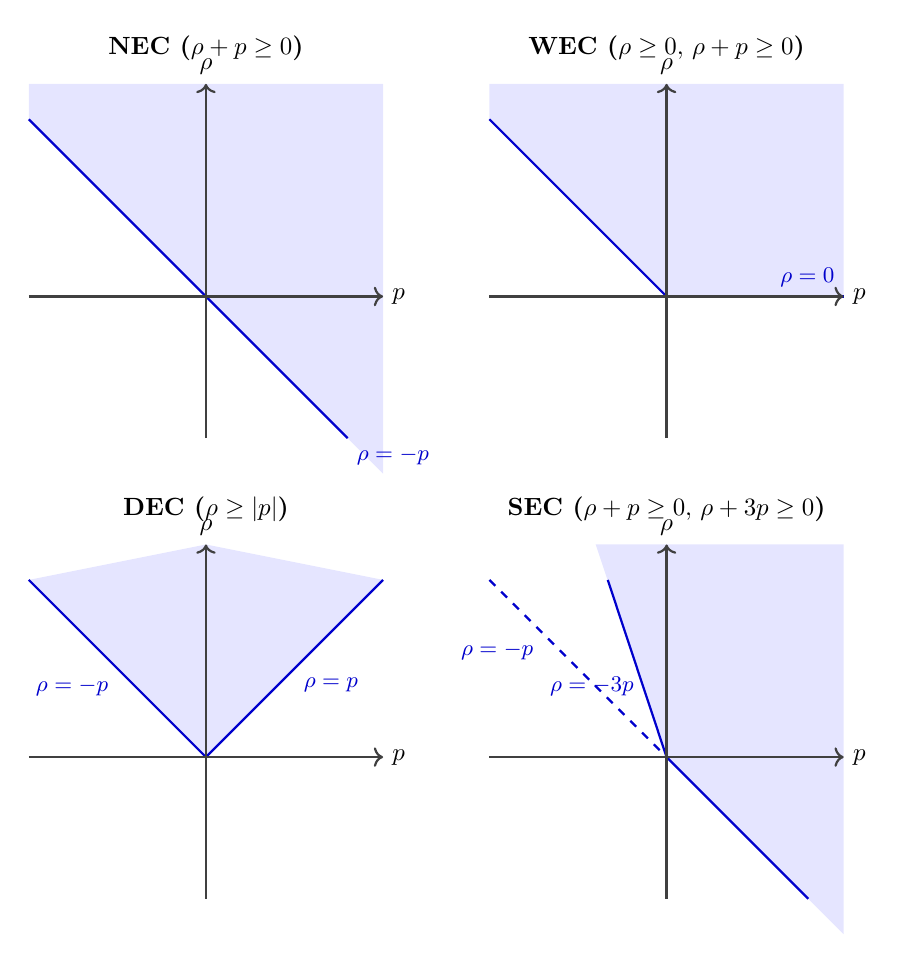
\begin{tikzpicture}[scale=0.9, every node/.style={scale=0.9}]
  % Common axes macro
  \def\drawaxes{
    \draw[->, thick, darkgray] (-2.5,0) -- (2.5,0) node[right, text=black] {$p$};
    \draw[->, thick, darkgray] (0,-2) -- (0,3) node[above, text=black] {$\rho$};
  }

  % NEC (Null Energy Condition)
  \begin{scope}[shift={(0, 6.5)}]
    \fill[blue!10] (-2.5, 2.5) -- (2.5, -2.5) -- (2.5, 3) -- (-2.5, 3) -- cycle;
    \draw[thick, blue!80!black] (-2.5, 2.5) -- (2.0, -2.0) node[below right, font=\small] {$\rho = -p$};
    \drawaxes
    \node[font=\bfseries] at (0, 3.5) {NEC ($\rho + p \ge 0$)};
  \end{scope}

  % WEC (Weak Energy Condition)
  \begin{scope}[shift={(6.5, 6.5)}]
    \fill[blue!10] (-2.5, 2.5) -- (0, 0) -- (2.5, 0) -- (2.5, 3) -- (-2.5, 3) -- cycle;
    \draw[thick, blue!80!black] (-2.5, 2.5) -- (0, 0);
    \draw[thick, blue!80!black] (0, 0) -- (2.5, 0) node[above left, font=\small] {$\rho = 0$};
    \drawaxes
    \node[font=\bfseries] at (0, 3.5) {WEC ($\rho \ge 0, \, \rho + p \ge 0$)};
  \end{scope}

  % DEC (Dominant Energy Condition)
  \begin{scope}[shift={(0, 0)}]
    \fill[blue!10] (0,0) -- (2.5, 2.5) -- (0, 3) -- (-2.5, 2.5) -- cycle;
    \draw[thick, blue!80!black] (-2.5, 2.5) -- (0, 0) node[midway, below left, font=\small] {$\rho = -p$};
    \draw[thick, blue!80!black] (0, 0) -- (2.5, 2.5) node[midway, below right, font=\small] {$\rho = p$};
    \drawaxes
    \node[font=\bfseries] at (0, 3.5) {DEC ($\rho \ge |p|$)};
  \end{scope}

  % SEC (Strong Energy Condition)
  \begin{scope}[shift={(6.5, 0)}]
    \fill[blue!10] (-1.0, 3) -- (0,0) -- (2.5, -2.5) -- (2.5, 3) -- cycle;
    \draw[thick, blue!80!black, dashed] (-2.5, 2.5) -- (0, 0) node[pos=0.3, below left, font=\small] {$\rho = -p$};
    \draw[thick, blue!80!black] (-0.83, 2.5) -- (0, 0) node[pos=0.6, left, font=\small] {$\rho = -3p$};
    \draw[thick, blue!80!black] (0,0) -- (2.0, -2.0);
    \drawaxes
    \node[font=\bfseries] at (0, 3.5) {SEC ($\rho + p \ge 0, \, \rho + 3p \ge 0$)};
  \end{scope}
\end{tikzpicture}
\end{center}



\subsubsection*{The SEC and Gravitational Attraction}
\begin{align}
R_{\mu\nu} t^{\mu} t^{\nu} &= 8\pi G \left( T_{\mu\nu} t^{\mu} t^{\nu} - \frac{1}{2} T g_{\mu\nu} t^{\mu} t^{\nu} \right) \nonumber \\
&= 8\pi G \left( T_{\mu\nu} t^{\mu} t^{\nu} - \frac{1}{2} T t_{\sigma} t^{\sigma} \right).
\end{align}
\begin{equation}
T_{\mu\nu} t^{\mu} t^{\nu} - \frac{1}{2} T t_{\sigma} t^{\sigma} \ge 0 \implies T_{\mu\nu} t^{\mu} t^{\nu} \ge \frac{1}{2} T t_{\sigma} t^{\sigma}.
\end{equation}

\section{The Equivalence Principle Revisited}
\subsection{The Approximation of Minimal Coupling}
\begin{equation}
\label{eq:minimal_scalar}
S_{\text{min}} = \int d^{4}x \sqrt{-g} \left[ -\frac{1}{2} g^{\mu\nu} \nabla_{\mu}\phi \nabla_{\nu}\phi - \frac{1}{2}m^{2}\phi^{2} \right].
\end{equation}
\begin{equation}
\label{eq:nonminimal_scalar}
S_{\text{non-min}} = \int d^{4}x \sqrt{-g} \left[ \frac{1}{2} \xi R \phi^{2} \right],
\end{equation}

\section{Alternative Theories of Gravity}
\subsection{Higher-Order Actions: $f(R)$ Gravity}
\begin{equation}
\label{eq:fR_action}
S = \int d^{4}x \sqrt{-g} \left[ \frac{1}{16\pi G} f(R) + \mathcal{L}*{M} \right].
\end{equation}
\begin{equation}
\delta S*{f(R)} = \frac{1}{16\pi G} \int d^{4}x \left[ \delta(\sqrt{-g}) f(R) + \sqrt{-g} \delta(f(R)) \right].
\end{equation}
\begin{equation}
\delta S_{f(R)} = \frac{1}{16\pi G} \int d^{4}x \sqrt{-g} \left[ -\frac{1}{2}f(R)g_{\mu\nu}\delta g^{\mu\nu} + f'(R)\delta R \right],
\end{equation}
\begin{equation}
\label{eq:delta_R_expansion}
\delta R = R_{\mu\nu}\delta g^{\mu\nu} + g^{\mu\nu}\delta R_{\mu\nu}.
\end{equation}
\begin{equation}
\delta R_{\mu\nu} = \nabla_{\lambda}(\delta \Gamma^{\lambda}*{\mu\nu}) - \nabla*{\nu}(\delta \Gamma^{\lambda}*{\mu\lambda}).
\end{equation}
\begin{equation}
\label{eq:palatini_contracted}
g^{\mu\nu}\delta R*{\mu\nu} = \nabla_{\mu}\nabla_{\nu}(\delta g^{\mu\nu}) - \Box(g_{\mu\nu}\delta g^{\mu\nu}),
\end{equation}
\begin{equation}
\delta S_{f(R)} = \frac{1}{16\pi G} \int d^{4}x \sqrt{-g} \left[ f'(R)R_{\mu\nu} - \frac{1}{2}f(R)g_{\mu\nu} \right] \delta g^{\mu\nu} + \frac{1}{16\pi G} \int d^{4}x \sqrt{-g} f'(R) \left[ \nabla_{\mu}\nabla_{\nu} - g_{\mu\nu}\Box \right] \delta g^{\mu\nu}.
\end{equation}
\begin{equation}
\int d^{4}x \sqrt{-g} f'(R) \nabla_{\mu}\nabla_{\nu} (\delta g^{\mu\nu}) = \int d^{4}x \sqrt{-g} \left[ \nabla_{\mu}\nabla_{\nu} f'(R) \right] \delta g^{\mu\nu},
\end{equation}
\begin{equation}
\delta S_{f(R)} = \frac{1}{16\pi G} \int d^{4}x \sqrt{-g} \left[ f'(R)R_{\mu\nu} - \frac{1}{2}f(R)g_{\mu\nu} + \nabla_{\mu}\nabla_{\nu}f'(R) - g_{\mu\nu}\Box f'(R) \right] \delta g^{\mu\nu}.
\end{equation}
\begin{equation}
\label{eq:fR_field_equation}
f'(R)R_{\mu\nu} - \frac{1}{2}f(R)g_{\mu\nu} + \left( \nabla_{\mu}\nabla_{\nu} - g_{\mu\nu}\Box \right) f'(R) = 8\pi G T_{\mu\nu}.
\end{equation}

\subsection{Scalar-Tensor Theories}
\begin{equation}
S = \int d^{4}x \sqrt{-g} \left[ \phi R - \frac{\omega(\phi)}{\phi} g^{\mu\nu}\nabla_{\mu}\phi\nabla_{\nu}\phi - V(\phi) + \mathcal{L}_{M} \right],
\end{equation}

\subsection{Torsion and Non-Christoffel Connections}
\begin{equation}
T^{\rho}*{\ \mu\nu} = \Gamma^{\rho}*{\mu\nu} - \Gamma^{\rho}_{\nu\mu}.
\end{equation}

\subsection{Additional Tensor Fields and Geometric Generalizations}
\begin{equation}
\Gamma^{\rho}*{\mu\nu} = \mathring{\Gamma}^{\rho}*{\mu\nu} + C^{\rho}_{\mu\nu}.
\end{equation}

\section{Variational Derivations of Advanced Field Equations}
\subsection{The Electromagnetic Stress-Energy Tensor}
\begin{equation}
\label{eq:em_action}
S_{\text{EM}} = \int d^{4}x \sqrt{-g} \left( -\frac{1}{4} F^{\mu\nu}F_{\mu\nu} + A_{\mu}J^{\mu} \right),
\end{equation}
\begin{equation}
F^{\mu\nu}F_{\mu\nu} = g^{\mu\alpha}g^{\nu\beta}F_{\mu\nu}F_{\alpha\beta}.
\end{equation}
\begin{align}
\delta S_{\text{EM}} &= \delta \int d^{4}x \left[ \sqrt{-g} \left( -\frac{1}{4} g^{\mu\alpha}g^{\nu\beta}F_{\mu\nu}F_{\alpha\beta} \right) \right] \nonumber \\
&= \int d^{4}x \left[ (\delta\sqrt{-g})\left(-\frac{1}{4} F^{\mu\nu}F_{\mu\nu}\right) - \frac{1}{4}\sqrt{-g} \delta(g^{\mu\alpha}g^{\nu\beta}) F_{\mu\nu}F_{\alpha\beta} \right].
\end{align}
\begin{equation}
\delta(g^{\mu\alpha}g^{\nu\beta}) = (\delta g^{\mu\alpha})g^{\nu\beta} + g^{\mu\alpha}(\delta g^{\nu\beta}).
\end{equation}
\begin{align}
-\frac{1}{4}\sqrt{-g} \left[ (\delta g^{\mu\alpha})g^{\nu\beta}F_{\mu\nu}F_{\alpha\beta} + g^{\mu\alpha}(\delta g^{\nu\beta})F_{\mu\nu}F_{\alpha\beta} \right].
\end{align}
\begin{equation}
-\frac{1}{4}\sqrt{-g} \left[ \delta g^{\rho\sigma}(g^{\nu\beta}F_{\rho\nu}F_{\sigma\beta}) + \delta g^{\rho\sigma}(g^{\mu\alpha}F_{\mu\rho}F_{\alpha\sigma}) \right].
\end{equation}
\begin{equation}
-\frac{1}{4}\sqrt{-g} \left[ 2 \delta g^{\rho\sigma} F_{\rho}^{\ \beta} F_{\sigma\beta} \right] = -\frac{1}{2}\sqrt{-g} F_{\rho\lambda}F_{\sigma}^{\ \lambda} \delta g^{\rho\sigma}.
\end{equation}
\begin{equation}
\delta S_{\text{EM}} = \int d^{4}x \sqrt{-g} \left[ \frac{1}{8} g_{\rho\sigma} F_{\mu\nu}F^{\mu\nu} - \frac{1}{2} F_{\rho\lambda}F_{\sigma}^{\ \lambda} \right] \delta g^{\rho\sigma}.
\end{equation}
\begin{equation}
\label{eq:em_tensor_derived}
T_{\rho\sigma} = F_{\rho\lambda}F_{\sigma}^{\ \lambda} - \frac{1}{4} g_{\rho\sigma} F_{\mu\nu}F^{\mu\nu}.
\end{equation}

\subsection{The Palatini Formulation of General Relativity}
\begin{equation}
S[g, \Gamma] = \int d^{4}x \sqrt{-g} g^{\mu\nu} R_{\mu\nu}(\Gamma).
\end{equation}
\begin{equation}
\delta R_{\mu\nu} = \nabla_{\lambda}(\delta\Gamma^{\lambda}*{\mu\nu}) - \nabla*{\nu}(\delta\Gamma^{\lambda}*{\mu\lambda}).
\end{equation}
\begin{equation}
\delta*{\Gamma} S = \int d^{4}x \sqrt{-g} g^{\mu\nu} \left[ \nabla_{\lambda}(\delta\Gamma^{\lambda}*{\mu\nu}) - \nabla*{\nu}(\delta\Gamma^{\lambda}*{\mu\lambda}) \right] = 0.
\end{equation}
\begin{equation}
\int d^{4}x \sqrt{-g} f \nabla*{\lambda}V^{\lambda} = - \int d^{4}x \sqrt{-g} V^{\lambda} \nabla_{\lambda}f + \text{boundary terms}.
\end{equation}
\begin{equation}
\delta_{\Gamma} S = \int d^{4}x \left[ -\nabla_{\lambda}(\sqrt{-g}g^{\mu\nu}) \delta\Gamma^{\lambda}*{\mu\nu} + \nabla*{\nu}(\sqrt{-g}g^{\mu\nu}) \delta\Gamma^{\lambda}*{\mu\lambda} \right].
\end{equation}
\begin{equation}
\delta*{\Gamma} S = \int d^{4}x \left[ -\nabla_{\lambda}(\sqrt{-g}g^{\mu\nu}) + \delta^{\nu}*{\lambda} \nabla*{\sigma}(\sqrt{-g}g^{\mu\sigma}) \right] \delta\Gamma^{\lambda}*{\mu\nu} = 0.
\end{equation}
\begin{equation}
\label{eq:palatini_bracket}
\nabla*{\lambda}(\sqrt{-g}g^{\mu\nu}) - \delta^{\nu}*{\lambda} \nabla*{\sigma}(\sqrt{-g}g^{\mu\sigma}) = 0.
\end{equation}
\begin{equation}
\nabla_{\sigma}(\sqrt{-g}g^{\mu\sigma}) - 4 \nabla_{\sigma}(\sqrt{-g}g^{\mu\sigma}) = 0 \implies -3 \nabla_{\sigma}(\sqrt{-g}g^{\mu\sigma}) = 0.
\end{equation}
\begin{equation}
\nabla_{\lambda}(\sqrt{-g}g^{\mu\nu}) = 0.
\end{equation}
\begin{equation}
\sqrt{-g} \nabla_{\lambda}g^{\mu\nu} + g^{\mu\nu} \nabla_{\lambda}\sqrt{-g} = 0.
\end{equation}
\begin{equation}
\nabla_{\lambda}g^{\mu\nu} = 0.
\end{equation}


\chapter{The Schwarzschild Solution}
\section{The Schwarzschild Solution}

\subsection{Metric Ansatz and Symmetry Justification}
To describe the exterior gravitational field of a static, spherically symmetric mass, we start with Minkowski space:
\begin{equation}
ds_{\text{Minkowski}}^2 = -dt^2 + dr^2 + r^2 d\Omega^2,
\end{equation}
\begin{equation}
d\Omega^2 = d\theta^2 + \sin^2\theta , d\phi^2.
\end{equation}
Imposing a static condition requires $t$-independence and time-reversal invariance ($t \rightarrow -t, dt \rightarrow -dt$) on a generic metric:
\begin{equation}
ds^2 = g_{tt} dt^2 + 2 g_{ti} dt dx^i + g_{ij} dx^i dx^j.
\end{equation}
\begin{equation}
ds^2 = g_{tt} (-dt)^2 + 2 g_{ti} (-dt) dx^i + g_{ij} dx^i dx^j,
\end{equation}
\begin{equation}
ds^2 = g_{tt} dt^2 - 2 g_{ti} dt dx^i + g_{ij} dx^i dx^j.
\end{equation}
Invariance demands:
\begin{equation}
2 g_{ti} dt dx^i = -2 g_{ti} dt dx^i.
\end{equation}
Thus $g_{ti} = 0$. Spherical symmetry limits angular dependence to $d\Omega^2$. To maintain a Lorentzian signature, we write the remaining components as exponentials:
\begin{equation}
ds^2 = -e^{2\alpha(r)} dt^2 + e^{2\beta(r)} dr^2 + e^{2\gamma(r)} r^2 d\Omega^2.
\end{equation}
Absorbing $e^{2\gamma(r)}$ into a new radial coordinate $\overline{r} = e^{\gamma(r)} r$:
\begin{equation}
\overline{r} = e^{\gamma(r)} r.
\end{equation}
\begin{equation}
d\overline{r} = \frac{d}{dr} \left( e^{\gamma(r)} r \right) dr,
\end{equation}
\begin{equation}
d\overline{r} = \left( \frac{d}{dr} \left( e^{\gamma(r)} \right) r + e^{\gamma(r)} \frac{d}{dr} (r) \right) dr,
\end{equation}
\begin{equation}
d\overline{r} = \left( e^{\gamma(r)} \frac{d\gamma(r)}{dr} r + e^{\gamma(r)} \right) dr.
\end{equation}
\begin{equation}
d\overline{r} = e^{\gamma(r)} \left( 1 + r \frac{d\gamma(r)}{dr} \right) dr.
\end{equation}
\begin{equation}
dr = e^{-\gamma(r)} \left( 1 + r \frac{d\gamma(r)}{dr} \right)^{-1} d\overline{r}.
\end{equation}
\begin{equation}
dr^2 = e^{-2\gamma(r)} \left( 1 + r \frac{d\gamma(r)}{dr} \right)^{-2} d\overline{r}^2.
\end{equation}
Substituting back:
\begin{equation}
ds^2 = -e^{2\alpha(r)} dt^2 + e^{2\beta(r)} \left[ e^{-2\gamma(r)} \left( 1 + r \frac{d\gamma(r)}{dr} \right)^{-2} d\overline{r}^2 \right] + \overline{r}^2 d\Omega^2,
\end{equation}
\begin{equation}
ds^2 = -e^{2\alpha(r)} dt^2 + e^{2\beta(r) - 2\gamma(r)} \left( 1 + r \frac{d\gamma(r)}{dr} \right)^{-2} d\overline{r}^2 + \overline{r}^2 d\Omega^2.
\end{equation}
Grouping factors:
\begin{equation}
e^{2\overline{\beta}(\overline{r})} = e^{2\beta(r) - 2\gamma(r)} \left( 1 + r \frac{d\gamma(r)}{dr} \right)^{-2},
\end{equation}
\begin{equation}
ds^2 = -e^{2\overline{\alpha}(\overline{r})} dt^2 + e^{2\overline{\beta}(\overline{r})} d\overline{r}^2 + \overline{r}^2 d\Omega^2.
\end{equation}
Dropping overbars gives the simplified general ansatz:
\begin{equation}
ds^2 = -e^{2\alpha(r)} dt^2 + e^{2\beta(r)} dr^2 + r^2 d\Omega^2.
\end{equation}

\subsection{Inverse Metric and Determinant}

\subsubsection{Covariant Metric Tensor Components}
\begin{equation}
ds^2 = g_{\mu\nu} dx^\mu dx^\nu = -e^{2\alpha(r)} dt^2 + e^{2\beta(r)} dr^2 + r^2 d\theta^2 + r^2 \sin^2\theta , d\phi^2.
\end{equation}
\begin{align}
g_{tt} &= -e^{2\alpha(r)}, \\
g_{rr} &= e^{2\beta(r)}, \\
g_{\theta\theta} &= r^2, \\
g_{\phi\phi} &= r^2 \sin^2\theta.
\end{align}
\begin{equation}
g_{\mu\nu} = 0 \quad \text{for} \quad \mu \neq \nu.
\end{equation}
\begin{equation}
g_{\mu\nu} = \begin{pmatrix}
-e^{2\alpha(r)} & 0 & 0 & 0 \\
0 & e^{2\beta(r)} & 0 & 0 \\
0 & 0 & r^2 & 0 \\
0 & 0 & 0 & r^2 \sin^2\theta
\end{pmatrix}.
\end{equation}

\subsubsection{Computation of the Inverse Metric Tensor}
\begin{equation}
g^{\mu\lambda} g_{\lambda\nu} = \delta^\mu_\nu,
\end{equation}
\begin{equation}
\sum_{\lambda} g^{t\lambda} g_{\lambda t} = \delta^t_t.
\end{equation}
\begin{equation}
g^{tt} g_{tt} + g^{tr} g_{rt} + g^{t\theta} g_{\theta t} + g^{t\phi} g_{\phi t} = 1.
\end{equation}
\begin{equation}
g^{tt} g_{tt} = 1.
\end{equation}
\begin{equation}
g^{tt} \left( -e^{2\alpha(r)} \right) = 1.
\end{equation}
\begin{equation}
g^{tt} = \frac{1}{-e^{2\alpha(r)}}.
\end{equation}
\begin{equation}
g^{tt} = -e^{-2\alpha(r)}.
\end{equation}
\begin{align}
g^{rr} g_{rr} &= 1, \\
g^{\theta\theta} g_{\theta\theta} &= 1, \\
g^{\phi\phi} g_{\phi\phi} &= 1.
\end{align}
\begin{align}
g^{rr} &= \frac{1}{g_{rr}} = \frac{1}{e^{2\beta(r)}} = e^{-2\beta(r)}, \\
g^{\theta\theta} &= \frac{1}{g_{\theta\theta}} = \frac{1}{r^2}, \\
g^{\phi\phi} &= \frac{1}{g_{\phi\phi}} = \frac{1}{r^2 \sin^2\theta}.
\end{align}
\begin{equation}
\sum_{\lambda} g^{t\lambda} g_{\lambda r} = \delta^t_r.
\end{equation}
\begin{equation}
g^{tt} g_{tr} + g^{tr} g_{rr} + g^{t\theta} g_{\theta r} + g^{t\phi} g_{\phi r} = 0.
\end{equation}
\begin{equation}
g^{tr} g_{rr} = 0.
\end{equation}
\begin{equation}
g^{tr} = 0.
\end{equation}
\begin{equation}
g^{\mu\nu} = \begin{pmatrix}
-e^{-2\alpha(r)} & 0 & 0 & 0 \\
0 & e^{-2\beta(r)} & 0 & 0 \\
0 & 0 & \frac{1}{r^2} & 0 \\
0 & 0 & 0 & \frac{1}{r^2 \sin^2\theta}
\end{pmatrix}.
\end{equation}

\subsubsection{Verification of the Inverse Metric via Matrix Multiplication}
\begin{equation}
g^{\mu\lambda} g_{\lambda\nu} = \begin{pmatrix}
-e^{-2\alpha(r)} & 0 & 0 & 0 \\
0 & e^{-2\beta(r)} & 0 & 0 \\
0 & 0 & \frac{1}{r^2} & 0 \\
0 & 0 & 0 & \frac{1}{r^2 \sin^2\theta}
\end{pmatrix}
\begin{pmatrix}
-e^{2\alpha(r)} & 0 & 0 & 0 \\
0 & e^{2\beta(r)} & 0 & 0 \\
0 & 0 & r^2 & 0 \\
0 & 0 & 0 & r^2 \sin^2\theta
\end{pmatrix}.
\end{equation}
\begin{align}
(g \cdot g)*{tt} &= \left(-e^{-2\alpha(r)}\right)\left(-e^{2\alpha(r)}\right) + 0 + 0 + 0, \\
(g \cdot g)*{rr} &= 0 + \left(e^{-2\beta(r)}\right)\left(e^{2\beta(r)}\right) + 0 + 0, \\
(g \cdot g)*{\theta\theta} &= 0 + 0 + \left(\frac{1}{r^2}\right)\left(r^2\right) + 0, \\
(g \cdot g)*{\phi\phi} &= 0 + 0 + 0 + \left(\frac{1}{r^2 \sin^2\theta}\right)\left(r^2 \sin^2\theta\right).
\end{align}
\begin{align}
(g \cdot g)*{tt} &= e^{-2\alpha(r) + 2\alpha(r)} = e^0 = 1, \\
(g \cdot g)*{rr} &= e^{-2\beta(r) + 2\beta(r)} = e^0 = 1, \\
(g \cdot g)*{\theta\theta} &= 1, \\
(g \cdot g)*{\phi\phi} &= 1.
\end{align}
\begin{equation}
g^{\mu\lambda} g_{\lambda\nu} = \begin{pmatrix}
1 & 0 & 0 & 0 \\
0 & 1 & 0 & 0 \\
0 & 0 & 1 & 0 \\
0 & 0 & 0 & 1
\end{pmatrix} = \delta^\mu_\nu.
\end{equation}

\subsubsection{Computation of the Metric Determinant}
\begin{equation}
g = g_{tt} g_{rr} g_{\theta\theta} g_{\phi\phi}.
\end{equation}
\begin{equation}
g = \left( -e^{2\alpha(r)} \right) \left( e^{2\beta(r)} \right) \left( r^2 \right) \left( r^2 \sin^2\theta \right).
\end{equation}
\begin{equation}
g = - \left( e^{2\alpha(r)} e^{2\beta(r)} \right) \left( r^2 \cdot r^2 \right) \left( \sin^2\theta \right).
\end{equation}
\begin{equation}
g = - e^{2\alpha(r) + 2\beta(r)} r^4 \sin^2\theta.
\end{equation}
\begin{equation}
g = - e^{2(\alpha(r) + \beta(r))} r^4 \sin^2\theta.
\end{equation}

\subsubsection{Computation of the Invariant Volume Element Factor}
\begin{equation}
-g = - \left( - e^{2(\alpha(r) + \beta(r))} r^4 \sin^2\theta \right).
\end{equation}
\begin{equation}
-g = e^{2(\alpha(r) + \beta(r))} r^4 \sin^2\theta.
\end{equation}
\begin{equation}
\sqrt{-g} = \sqrt{e^{2(\alpha(r) + \beta(r))} r^4 \sin^2\theta}.
\end{equation}
\begin{equation}
\sqrt{-g} = \left( e^{2(\alpha(r) + \beta(r))} \right)^{\frac{1}{2}} \left( r^4 \right)^{\frac{1}{2}} \left( \sin^2\theta \right)^{\frac{1}{2}}.
\end{equation}
\begin{align}
\left( e^{2(\alpha(r) + \beta(r))} \right)^{\frac{1}{2}} &= e^{\alpha(r) + \beta(r)}, \\
\left( r^4 \right)^{\frac{1}{2}} &= r^2, \\
\left( \sin^2\theta \right)^{\frac{1}{2}} &= \sin\theta.
\end{align}
\begin{equation}
\sqrt{-g} = e^{\alpha(r) + \beta(r)} r^2 \sin\theta.
\end{equation}

\subsection*{Deriving Christoffel Symbols via the Lagrangian Method}
Using $\mathcal{L} = g_{\mu\nu} \dot{x}^\mu \dot{x}^\nu$:
\begin{equation}
\mathcal{L} = g_{\mu\nu} \dot{x}^\mu \dot{x}^\nu
\end{equation}
\begin{equation}
\mathcal{L} = -e^{2\alpha(t,r)} \dot{t}^2 + e^{2\beta(t,r)} \dot{r}^2 + r^2 \dot{\theta}^2 + r^2 \sin^2\theta \dot{\phi}^2
\end{equation}
Euler-Lagrange equations yield geodesics:
\begin{equation}
\frac{d}{d\lambda} \left( \frac{\partial \mathcal{L}}{\partial \dot{x}^\mu} \right) - \frac{\partial \mathcal{L}}{\partial x^\mu} = 0 \label{eq:EL_general}
\end{equation}
\begin{equation}
\ddot{x}^\mu + \Gamma^\mu_{\rho\sigma} \dot{x}^\rho \dot{x}^\sigma = 0 \label{eq:geodesic_general}
\end{equation}

\subsubsection*{1. The $t$-equation}
\begin{equation}
\frac{\partial \mathcal{L}}{\partial \dot{t}} = -2e^{2\alpha(t,r)} \dot{t}
\end{equation}
\begin{align}
\frac{d}{d\lambda} \left( \frac{\partial \mathcal{L}}{\partial \dot{t}} \right) &= -2 \frac{d}{d\lambda} \left( e^{2\alpha(t,r)} \right) \dot{t} - 2e^{2\alpha(t,r)} \ddot{t} \nonumber \\
&= -2 \left( e^{2\alpha(t,r)} \cdot 2 \left[ \frac{\partial \alpha}{\partial t} \dot{t} + \frac{\partial \alpha}{\partial r} \dot{r} \right] \right) \dot{t} - 2e^{2\alpha(t,r)} \ddot{t} \nonumber \\
&= -4e^{2\alpha(t,r)} \partial_t \alpha , \dot{t}^2 - 4e^{2\alpha(t,r)} \partial_r \alpha , \dot{t}\dot{r} - 2e^{2\alpha(t,r)} \ddot{t}
\end{align}
\begin{equation}
\frac{\partial \mathcal{L}}{\partial t} = -2\dot{t}^2 e^{2\alpha(t,r)} \partial_t \alpha + 2\dot{r}^2 e^{2\beta(t,r)} \partial_t \beta
\end{equation}
\begin{equation}
-2e^{2\alpha(t,r)} \ddot{t} - 4e^{2\alpha(t,r)} \partial_t \alpha , \dot{t}^2 - 4e^{2\alpha(t,r)} \partial_r \alpha , \dot{t}\dot{r} - \left( -2e^{2\alpha(t,r)} \partial_t \alpha , \dot{t}^2 + 2e^{2\beta(t,r)} \partial_t \beta , \dot{r}^2 \right) = 0
\end{equation}
\begin{equation}
\ddot{t} + 2\partial_t \alpha , \dot{t}^2 + 2\partial_r \alpha , \dot{t}\dot{r} - \partial_t \alpha , \dot{t}^2 + e^{2(\beta - \alpha)} \partial_t \beta , \dot{r}^2 = 0
\end{equation}
\begin{equation}
\ddot{t} + (\partial_t \alpha) \dot{t}^2 + e^{2(\beta - \alpha)} (\partial_t \beta) \dot{r}^2 + 2 (\partial_r \alpha) \dot{t}\dot{r} = 0 \label{eq:geo_t}
\end{equation}
\begin{equation}
\ddot{t} + \Gamma^t_{tt}\dot{t}^2 + \Gamma^t_{rr}\dot{r}^2 + \Gamma^t_{\theta\theta}\dot{\theta}^2 + \Gamma^t_{\phi\phi}\dot{\phi}^2 + 2\Gamma^t_{tr}\dot{t}\dot{r} + \dots = 0
\end{equation}
\begin{align}
\Gamma^t_{tt} &= \partial_t \alpha \\
\Gamma^t_{rr} &= e^{2(\beta - \alpha)} \partial_t \beta \\
\Gamma^t_{tr} &= \partial_r \alpha
\end{align}

\subsubsection*{2. The $r$-equation}
\begin{equation}
\frac{\partial \mathcal{L}}{\partial \dot{r}} = 2e^{2\beta(t,r)} \dot{r}
\end{equation}
\begin{align}
\frac{d}{d\lambda} \left( \frac{\partial \mathcal{L}}{\partial \dot{r}} \right) &= 2 \left( e^{2\beta(t,r)} \cdot 2 \left[ \frac{\partial \beta}{\partial t} \dot{t} + \frac{\partial \beta}{\partial r} \dot{r} \right] \right) \dot{r} + 2e^{2\beta(t,r)} \ddot{r} \nonumber \\
&= 4e^{2\beta(t,r)} \partial_t \beta , \dot{t}\dot{r} + 4e^{2\beta(t,r)} \partial_r \beta , \dot{r}^2 + 2e^{2\beta(t,r)} \ddot{r}
\end{align}
\begin{equation}
\frac{\partial \mathcal{L}}{\partial r} = -2\dot{t}^2 e^{2\alpha(t,r)} \partial_r \alpha + 2\dot{r}^2 e^{2\beta(t,r)} \partial_r \beta + 2r\dot{\theta}^2 + 2r\sin^2\theta \dot{\phi}^2
\end{equation}
\begin{equation}
2e^{2\beta} \ddot{r} + 4e^{2\beta} \partial_t \beta , \dot{t}\dot{r} + 4e^{2\beta} \partial_r \beta , \dot{r}^2 - \left( -2e^{2\alpha} \partial_r \alpha , \dot{t}^2 + 2e^{2\beta} \partial_r \beta , \dot{r}^2 + 2r\dot{\theta}^2 + 2r\sin^2\theta \dot{\phi}^2 \right) = 0
\end{equation}
\begin{equation}
\ddot{r} + 2\partial_t \beta , \dot{t}\dot{r} + 2\partial_r \beta , \dot{r}^2 + e^{2(\alpha - \beta)} \partial_r \alpha , \dot{t}^2 - \partial_r \beta , \dot{r}^2 - r e^{-2\beta} \dot{\theta}^2 - r \sin^2\theta e^{-2\beta} \dot{\phi}^2 = 0
\end{equation}
\begin{equation}
\ddot{r} + e^{2(\alpha - \beta)} (\partial_r \alpha) \dot{t}^2 + (\partial_r \beta) \dot{r}^2 - r e^{-2\beta} \dot{\theta}^2 - r \sin^2\theta e^{-2\beta} \dot{\phi}^2 + 2 (\partial_t \beta) \dot{t}\dot{r} = 0 \label{eq:geo_r}
\end{equation}
\begin{equation}
\ddot{r} + \Gamma^r_{tt}\dot{t}^2 + \Gamma^r_{rr}\dot{r}^2 + \Gamma^r_{\theta\theta}\dot{\theta}^2 + \Gamma^r_{\phi\phi}\dot{\phi}^2 + 2\Gamma^r_{tr}\dot{t}\dot{r} + \dots = 0
\end{equation}
\begin{align}
\Gamma^r_{tt} &= e^{2(\alpha - \beta)} \partial_r \alpha \\
\Gamma^r_{rr} &= \partial_r \beta \\
\Gamma^r_{\theta\theta} &= -r e^{-2\beta} \\
\Gamma^r_{\phi\phi} &= -r e^{-2\beta} \sin^2\theta \\
\Gamma^r_{tr} &= \partial_t \beta
\end{align}

\subsubsection*{3. The $\theta$-equation}
\begin{equation}
\frac{\partial \mathcal{L}}{\partial \dot{\theta}} = 2r^2 \dot{\theta}
\end{equation}
\begin{equation}
\frac{d}{d\lambda} \left( \frac{\partial \mathcal{L}}{\partial \dot{\theta}} \right) = 4r\dot{r}\dot{\theta} + 2r^2 \ddot{\theta}
\end{equation}
\begin{equation}
\frac{\partial \mathcal{L}}{\partial \theta} = 2r^2 \sin\theta \cos\theta , \dot{\phi}^2
\end{equation}
\begin{equation}
2r^2 \ddot{\theta} + 4r\dot{r}\dot{\theta} - 2r^2 \sin\theta \cos\theta , \dot{\phi}^2 = 0
\end{equation}
\begin{equation}
\ddot{\theta} + (-\sin\theta \cos\theta) \dot{\phi}^2 + 2 \left(\frac{1}{r}\right) \dot{r}\dot{\theta} = 0 \label{eq:geo_theta}
\end{equation}
\begin{equation}
\ddot{\theta} + \Gamma^\theta_{\phi\phi}\dot{\phi}^2 + 2\Gamma^\theta_{r\theta}\dot{r}\dot{\theta} + \dots = 0
\end{equation}
\begin{align}
\Gamma^\theta_{\phi\phi} &= -\sin\theta \cos\theta \\
\Gamma^\theta_{r\theta} &= \frac{1}{r}
\end{align}
\subsubsection*{4. The $\phi$-equation}
\begin{equation}
\frac{\partial \mathcal{L}}{\partial \dot{\phi}} = 2r^2 \sin^2\theta , \dot{\phi}
\end{equation}
\begin{align}
\frac{d}{d\lambda} \left( \frac{\partial \mathcal{L}}{\partial \dot{\phi}} \right) &= 2 \frac{d}{d\lambda} (r^2 \sin^2\theta) \dot{\phi} + 2r^2 \sin^2\theta , \ddot{\phi} \nonumber \\
&= 2 \left( 2r\dot{r} \sin^2\theta + r^2 (2\sin\theta\cos\theta)\dot{\theta} \right) \dot{\phi} + 2r^2 \sin^2\theta , \ddot{\phi} \nonumber \\
&= 4r\sin^2\theta , \dot{r}\dot{\phi} + 4r^2 \sin\theta \cos\theta , \dot{\theta}\dot{\phi} + 2r^2 \sin^2\theta , \ddot{\phi}
\end{align}
\begin{equation}
\frac{\partial \mathcal{L}}{\partial \phi} = 0
\end{equation}
\begin{equation}
2r^2 \sin^2\theta , \ddot{\phi} + 4r\sin^2\theta , \dot{r}\dot{\phi} + 4r^2 \sin\theta \cos\theta , \dot{\theta}\dot{\phi} = 0
\end{equation}
\begin{equation}
\ddot{\phi} + \frac{2}{r} \dot{r}\dot{\phi} + 2 \frac{\cos\theta}{\sin\theta} \dot{\theta}\dot{\phi} = 0
\end{equation}
\begin{equation}
\ddot{\phi} + 2 \left(\frac{1}{r}\right) \dot{r}\dot{\phi} + 2 (\cot\theta) \dot{\theta}\dot{\phi} = 0 \label{eq:geo_phi}
\end{equation}
\begin{equation}
\ddot{\phi} + 2\Gamma^\phi_{r\phi}\dot{r}\dot{\phi} + 2\Gamma^\phi_{\theta\phi}\dot{\theta}\dot{\phi} + \dots = 0
\end{equation}
\begin{align}
\Gamma^\phi_{r\phi} &= \frac{1}{r} \\
\Gamma^\phi_{\theta\phi} &= \cot\theta
\end{align}

\subsubsection*{5. Summary}
\begin{align}
\Gamma^t_{tt} &= \partial_t \alpha \\
\Gamma^t_{rr} &= e^{2(\beta - \alpha)} \partial_t \beta \\
\Gamma^t_{tr} &= \partial_r \alpha \\
\Gamma^r_{tt} &= e^{2(\alpha - \beta)} \partial_r \alpha \\
\Gamma^r_{rr} &= \partial_r \beta \\
\Gamma^r_{tr} &= \partial_t \beta \\
\Gamma^r_{\theta\theta} &= -r e^{-2\beta} \\
\Gamma^r_{\phi\phi} &= -r e^{-2\beta} \sin^2\theta \\
\Gamma^\theta_{r\theta} &= \frac{1}{r} \\
\Gamma^\theta_{\phi\phi} &= -\sin\theta \cos\theta \\
\Gamma^\phi_{r\phi} &= \frac{1}{r} \\
\Gamma^\phi_{\theta\phi} &= \cot\theta
\end{align}

\subsection{Derivation of the Ricci Tensor}
\begin{equation}
R_{\mu\nu} = {R^\lambda}*{\mu\lambda\nu} = \partial*\lambda \Gamma^\lambda_{\mu\nu} - \partial_\nu \Gamma^\lambda_{\mu\lambda} + \Gamma^\lambda_{\sigma\lambda} \Gamma^\sigma_{\mu\nu} - \Gamma^\lambda_{\sigma\nu} \Gamma^\sigma_{\mu\lambda}.
\end{equation}
\begin{equation}
\Gamma^\lambda_{\mu\lambda} = \partial_\mu \ln \sqrt{-g}.
\end{equation}
\begin{equation}
\sqrt{-g} = e^{\alpha(r) + \beta(r)} r^2 \sin\theta.
\end{equation}
\begin{equation}
\ln \sqrt{-g} = \alpha(r) + \beta(r) + 2\ln r + \ln(\sin\theta).
\end{equation}
\begin{equation}
\Gamma^\lambda_{r\lambda} = \partial_r \left[ \alpha(r) + \beta(r) + 2\ln r + \ln(\sin\theta) \right].
\end{equation}
\begin{equation}
\Gamma^\lambda_{r\lambda} = \partial_r\alpha + \partial_r\beta + \frac{2}{r}.
\end{equation}
\begin{equation}
\Gamma^\lambda_{\theta\lambda} = \partial_\theta \left[ \alpha(r) + \beta(r) + 2\ln r + \ln(\sin\theta) \right].
\end{equation}
\begin{equation}
\Gamma^\lambda_{\theta\lambda} = \frac{1}{\sin\theta} \cos\theta = \cot\theta.
\end{equation}

\subsubsection{Temporal Component: $R_{tt}$}
\begin{equation}
R_{tt} = \partial_\lambda \Gamma^\lambda_{tt} - \partial_t \Gamma^\lambda_{t\lambda} + \Gamma^\lambda_{\sigma\lambda} \Gamma^\sigma_{tt} - \Gamma^\lambda_{\sigma t} \Gamma^\sigma_{t\lambda}.
\end{equation}
\begin{equation}
\partial_\lambda \Gamma^\lambda_{tt} = \partial_r \Gamma^r_{tt}.
\end{equation}
\begin{equation}
\partial_r \Gamma^r_{tt} = \partial_r \left( e^{2(\alpha-\beta)} \partial_r\alpha \right).
\end{equation}
\begin{equation}
\partial_r \Gamma^r_{tt} = 2(\partial_r\alpha - \partial_r\beta)e^{2(\alpha-\beta)}\partial_r\alpha + e^{2(\alpha-\beta)}\partial_r^2\alpha.
\end{equation}
\begin{equation}
\partial_r \Gamma^r_{tt} = e^{2(\alpha-\beta)} \left[ 2(\partial_r\alpha)^2 - 2\partial_r\alpha\partial_r\beta + \partial_r^2\alpha \right].
\end{equation}
\begin{equation}
\Gamma^\lambda_{\sigma\lambda} \Gamma^\sigma_{tt} = \Gamma^\lambda_{r\lambda} \Gamma^r_{tt}.
\end{equation}
\begin{equation}
\Gamma^\lambda_{r\lambda} \Gamma^r_{tt} = \left( \partial_r\alpha + \partial_r\beta + \frac{2}{r} \right) \left( e^{2(\alpha-\beta)} \partial_r\alpha \right).
\end{equation}
\begin{equation}
\Gamma^\lambda_{r\lambda} \Gamma^r_{tt} = e^{2(\alpha-\beta)} \left[ (\partial_r\alpha)^2 + \partial_r\alpha\partial_r\beta + \frac{2}{r}\partial_r\alpha \right].
\end{equation}
\begin{equation}
-\Gamma^\lambda_{\sigma t} \Gamma^\sigma_{t\lambda} = -\left( \Gamma^t_{rt} \Gamma^r_{tt} + \Gamma^r_{tt} \Gamma^t_{tr} \right).
\end{equation}
\begin{equation}
-\Gamma^\lambda_{\sigma t} \Gamma^\sigma_{t\lambda} = -2 \Gamma^t_{tr} \Gamma^r_{tt}.
\end{equation}
\begin{equation}
-\Gamma^\lambda_{\sigma t} \Gamma^\sigma_{t\lambda} = -2 (\partial_r\alpha) \left( e^{2(\alpha-\beta)} \partial_r\alpha \right) = e^{2(\alpha-\beta)} \left[ -2(\partial_r\alpha)^2 \right].
\end{equation}
\begin{align}
R_{tt} &= e^{2(\alpha-\beta)} \left[ 2(\partial_r\alpha)^2 - 2\partial_r\alpha\partial_r\beta + \partial_r^2\alpha \right] \nonumber \\
&\quad + e^{2(\alpha-\beta)} \left[ (\partial_r\alpha)^2 + \partial_r\alpha\partial_r\beta + \frac{2}{r}\partial_r\alpha \right] \nonumber \\
&\quad + e^{2(\alpha-\beta)} \left[ -2(\partial_r\alpha)^2 \right].
\end{align}
\begin{equation}
R_{tt} = e^{2(\alpha-\beta)} \left[ \partial_r^2\alpha + (\partial_r\alpha)^2 - \partial_r\alpha\partial_r\beta + \frac{2}{r}\partial_r\alpha \right].
\end{equation}

\subsubsection{Radial Component: $R_{rr}$}
\begin{equation}
R_{rr} = \partial_\lambda \Gamma^\lambda_{rr} - \partial_r \Gamma^\lambda_{r\lambda} + \Gamma^\lambda_{\sigma\lambda} \Gamma^\sigma_{rr} - \Gamma^\lambda_{\sigma r} \Gamma^\sigma_{r\lambda}.
\end{equation}
\begin{equation}
\partial_\lambda \Gamma^\lambda_{rr} = \partial_r \Gamma^r_{rr} = \partial_r (\partial_r\beta) = \partial_r^2\beta.
\end{equation}
\begin{equation}
-\partial_r \Gamma^\lambda_{r\lambda} = -\partial_r \left( \partial_r\alpha + \partial_r\beta + \frac{2}{r} \right) = -\partial_r^2\alpha - \partial_r^2\beta + \frac{2}{r^2}.
\end{equation}
\begin{equation}
\Gamma^\lambda_{\sigma\lambda} \Gamma^\sigma_{rr} = \Gamma^\lambda_{r\lambda} \Gamma^r_{rr}.
\end{equation}
\begin{equation}
\Gamma^\lambda_{r\lambda} \Gamma^r_{rr} = \left( \partial_r\alpha + \partial_r\beta + \frac{2}{r} \right) (\partial_r\beta) = \partial_r\alpha\partial_r\beta + (\partial_r\beta)^2 + \frac{2}{r}\partial_r\beta.
\end{equation}
\begin{equation}
-\Gamma^\lambda_{\sigma r} \Gamma^\sigma_{r\lambda} = -\left( \Gamma^t_{tr} \Gamma^t_{rt} + \Gamma^r_{rr} \Gamma^r_{rr} + \Gamma^\theta_{\theta r} \Gamma^\theta_{r\theta} + \Gamma^\phi_{\phi r} \Gamma^\phi_{r\phi} \right).
\end{equation}
\begin{equation}
-\Gamma^\lambda_{\sigma r} \Gamma^\sigma_{r\lambda} = -\left[ (\partial_r\alpha)^2 + (\partial_r\beta)^2 + \left(\frac{1}{r}\right)^2 + \left(\frac{1}{r}\right)^2 \right].
\end{equation}
\begin{equation}
-\Gamma^\lambda_{\sigma r} \Gamma^\sigma_{r\lambda} = -(\partial_r\alpha)^2 - (\partial_r\beta)^2 - \frac{2}{r^2}.
\end{equation}
\begin{align}
R_{rr} &= \partial_r^2\beta - \partial_r^2\alpha - \partial_r^2\beta + \frac{2}{r^2} \nonumber \\
&\quad + \partial_r\alpha\partial_r\beta + (\partial_r\beta)^2 + \frac{2}{r}\partial_r\beta \nonumber \\
&\quad - (\partial_r\alpha)^2 - (\partial_r\beta)^2 - \frac{2}{r^2}.
\end{align}
\begin{equation}
R_{rr} = -\partial_r^2\alpha - (\partial_r\alpha)^2 + \partial_r\alpha\partial_r\beta + \frac{2}{r}\partial_r\beta.
\end{equation}

\subsubsection{Polar Component: $R_{\theta\theta}$}
\begin{equation}
R_{\theta\theta} = \partial_\lambda \Gamma^\lambda_{\theta\theta} - \partial_\theta \Gamma^\lambda_{\theta\lambda} + \Gamma^\lambda_{\sigma\lambda} \Gamma^\sigma_{\theta\theta} - \Gamma^\lambda_{\sigma\theta} \Gamma^\sigma_{\theta\lambda}.
\end{equation}
\begin{equation}
\partial_\lambda \Gamma^\lambda_{\theta\theta} = \partial_r \Gamma^r_{\theta\theta} = \partial_r \left( -re^{-2\beta} \right).
\end{equation}
\begin{equation}
\partial_r \Gamma^r_{\theta\theta} = -e^{-2\beta} - r \left( -2\partial_r\beta e^{-2\beta} \right) = e^{-2\beta} \left( 2r\partial_r\beta - 1 \right).
\end{equation}
\begin{equation}
-\partial_\theta \Gamma^\lambda_{\theta\lambda} = -\partial_\theta (\cot\theta) = \csc^2\theta.
\end{equation}
\begin{equation}
\Gamma^\lambda_{\sigma\lambda} \Gamma^\sigma_{\theta\theta} = \Gamma^\lambda_{r\lambda} \Gamma^r_{\theta\theta}.
\end{equation}
\begin{equation}
\Gamma^\lambda_{r\lambda} \Gamma^r_{\theta\theta} = \left( \partial_r\alpha + \partial_r\beta + \frac{2}{r} \right) \left( -re^{-2\beta} \right) = e^{-2\beta} \left( -r\partial_r\alpha - r\partial_r\beta - 2 \right).
\end{equation}
\begin{equation}
-\Gamma^\lambda_{\sigma\theta} \Gamma^\sigma_{\theta\lambda} = -\left( \Gamma^\phi_{\phi\theta} \Gamma^\phi_{\theta\phi} + \Gamma^r_{\theta\theta} \Gamma^\theta_{\theta r} + \Gamma^\theta_{r\theta} \Gamma^r_{\theta\theta} \right).
\end{equation}
\begin{equation}
-\Gamma^\lambda_{\sigma\theta} \Gamma^\sigma_{\theta\lambda} = -\left[ (\cot\theta)^2 + \left( -re^{-2\beta} \right) \left(\frac{1}{r}\right) + \left(\frac{1}{r}\right) \left( -re^{-2\beta} \right) \right].
\end{equation}
\begin{equation}
-\Gamma^\lambda_{\sigma\theta} \Gamma^\sigma_{\theta\lambda} = -\cot^2\theta + 2e^{-2\beta}.
\end{equation}
\begin{equation}
R_{\theta\theta} = e^{-2\beta} \left( 2r\partial_r\beta - 1 \right) + \csc^2\theta + e^{-2\beta} \left( -r\partial_r\alpha - r\partial_r\beta - 2 \right) - \cot^2\theta + 2e^{-2\beta}.
\end{equation}
\begin{equation}
R_{\theta\theta} = e^{-2\beta} \left[ r\partial_r\beta - r\partial_r\alpha - 1 \right] + 1.
\end{equation}

\subsubsection{Azimuthal Component: $R_{\phi\phi}$}
\begin{equation}
R_{\phi\phi} = \partial_\lambda \Gamma^\lambda_{\phi\phi} - \partial_\phi \Gamma^\lambda_{\phi\lambda} + \Gamma^\lambda_{\sigma\lambda} \Gamma^\sigma_{\phi\phi} - \Gamma^\lambda_{\sigma\phi} \Gamma^\sigma_{\phi\lambda}.
\end{equation}
\begin{equation}
\partial_\lambda \Gamma^\lambda_{\phi\phi} = \partial_r \Gamma^r_{\phi\phi} + \partial_\theta \Gamma^\theta_{\phi\phi}.
\end{equation}
\begin{equation}
\partial_r \left( -re^{-2\beta}\sin^2\theta \right) = \sin^2\theta \left( -e^{-2\beta} + 2r\partial_r\beta e^{-2\beta} \right).
\end{equation}
\begin{equation}
\partial_\theta \left( -\sin\theta\cos\theta \right) = -\cos^2\theta + \sin^2\theta.
\end{equation}
\begin{equation}
-\partial_\phi \Gamma^\lambda_{\phi\lambda} = 0.
\end{equation}
\begin{equation}
\Gamma^\lambda_{\sigma\lambda} \Gamma^\sigma_{\phi\phi} = \Gamma^\lambda_{r\lambda} \Gamma^r_{\phi\phi} + \Gamma^\lambda_{\theta\lambda} \Gamma^\theta_{\phi\phi}.
\end{equation}
\begin{equation}
\Gamma^\lambda_{\sigma\lambda} \Gamma^\sigma_{\phi\phi} = \left( \partial_r\alpha + \partial_r\beta + \frac{2}{r} \right) \left( -re^{-2\beta}\sin^2\theta \right) + (\cot\theta) \left( -\sin\theta\cos\theta \right).
\end{equation}
\begin{equation}
\Gamma^\lambda_{\sigma\lambda} \Gamma^\sigma_{\phi\phi} = \sin^2\theta , e^{-2\beta} \left( -r\partial_r\alpha - r\partial_r\beta - 2 \right) - \cos^2\theta.
\end{equation}
\begin{equation}
-\Gamma^\lambda_{\sigma\phi} \Gamma^\sigma_{\phi\lambda} = -\left( \Gamma^r_{\phi\phi} \Gamma^\phi_{\phi r} + \Gamma^\phi_{r\phi} \Gamma^r_{\phi\phi} + \Gamma^\theta_{\phi\phi} \Gamma^\phi_{\phi\theta} + \Gamma^\phi_{\theta\phi} \Gamma^\theta_{\phi\phi} \right).
\end{equation}
\begin{equation}
-\Gamma^\lambda_{\sigma\phi} \Gamma^\sigma_{\phi\lambda} = -2\Gamma^r_{\phi\phi} \Gamma^\phi_{\phi r} - 2\Gamma^\theta_{\phi\phi} \Gamma^\phi_{\phi\theta}.
\end{equation}
\begin{equation}
-\Gamma^\lambda_{\sigma\phi} \Gamma^\sigma_{\phi\lambda} = -2\left( -re^{-2\beta}\sin^2\theta \right)\left(\frac{1}{r}\right) - 2\left(-\sin\theta\cos\theta\right)\left(\frac{\cos\theta}{\sin\theta}\right).
\end{equation}
\begin{equation}
-\Gamma^\lambda_{\sigma\phi} \Gamma^\sigma_{\phi\lambda} = 2e^{-2\beta}\sin^2\theta + 2\cos^2\theta.
\end{equation}
\begin{align}
R_{\phi\phi} &= \sin^2\theta \left( -e^{-2\beta} + 2r\partial_r\beta e^{-2\beta} \right) - \cos^2\theta + \sin^2\theta \nonumber \\
&\quad + \sin^2\theta , e^{-2\beta} \left( -r\partial_r\alpha - r\partial_r\beta - 2 \right) - \cos^2\theta \nonumber \\
&\quad + 2e^{-2\beta}\sin^2\theta + 2\cos^2\theta.
\end{align}
\begin{equation}
R_{\phi\phi} = \sin^2\theta \left[ e^{-2\beta} \left( -1 + 2r\partial_r\beta - r\partial_r\alpha - r\partial_r\beta - 2 + 2 \right) + 1 \right].
\end{equation}
\begin{equation}
R_{\phi\phi} = \sin^2\theta \left[ e^{-2\beta} \left( r\partial_r\beta - r\partial_r\alpha - 1 \right) + 1 \right].
\end{equation}

\subsection{Einstein Equations and Solution}
\begin{equation}
R_{\mu\nu} = 0.
\end{equation}
\begin{align}
R_{tt} &= e^{2(\alpha-\beta)} \left[ \partial_r^2\alpha + (\partial_r\alpha)^2 - \partial_r\alpha\partial_r\beta + \frac{2}{r}\partial_r\alpha \right] = 0, \\
R_{rr} &= -\partial_r^2\alpha - (\partial_r\alpha)^2 + \partial_r\alpha\partial_r\beta + \frac{2}{r}\partial_r\beta = 0, \\
R_{\theta\theta} &= e^{-2\beta} \left[ r(\partial_r\beta - \partial_r\alpha) - 1 \right] + 1 = 0.
\end{align}
\begin{equation}
e^{2(\beta-\alpha)} R_{tt} + R_{rr} = 0.
\end{equation}
\begin{align}
e^{2(\beta-\alpha)} R_{tt} + R_{rr} &= \left[ \partial_r^2\alpha + (\partial_r\alpha)^2 - \partial_r\alpha\partial_r\beta + \frac{2}{r}\partial_r\alpha \right] \nonumber \\
&\quad + \left[ -\partial_r^2\alpha - (\partial_r\alpha)^2 + \partial_r\alpha\partial_r\beta + \frac{2}{r}\partial_r\beta \right].
\end{align}
\begin{equation}
e^{2(\beta-\alpha)} R_{tt} + R_{rr} = \frac{2}{r}\partial_r\alpha + \frac{2}{r}\partial_r\beta = 0.
\end{equation}
\begin{equation}
\frac{2}{r} \left( \partial_r\alpha + \partial_r\beta \right) = 0.
\end{equation}
\begin{equation}
\partial_r \left( \alpha + \beta \right) = 0.
\end{equation}
\begin{equation}
\alpha(r) + \beta(r) = c,
\end{equation}
Absorbing the constant $c$:
\begin{equation}
\alpha(r) = -\beta(r).
\end{equation}
Substituting $\beta = -\alpha$:
\begin{equation}
e^{-2\beta} \left[ r(\partial_r\beta - \partial_r\alpha) - 1 \right] + 1 = 0.
\end{equation}
\begin{equation}
e^{2\alpha} \left[ r(-\partial_r\alpha - \partial_r\alpha) - 1 \right] + 1 = 0.
\end{equation}
\begin{equation}
e^{2\alpha} \left( -2r\partial_r\alpha - 1 \right) + 1 = 0.
\end{equation}
\begin{equation}
e^{2\alpha} \left( 2r\partial_r\alpha + 1 \right) = 1.
\end{equation}
\begin{equation}
\partial_r \left( r e^{2\alpha} \right) = \left( \partial_r r \right) e^{2\alpha} + r \left( \partial_r e^{2\alpha} \right).
\end{equation}
\begin{equation}
\partial_r \left( r e^{2\alpha} \right) = e^{2\alpha} + r \left( 2\partial_r\alpha , e^{2\alpha} \right).
\end{equation}
\begin{equation}
\partial_r \left( r e^{2\alpha} \right) = e^{2\alpha} \left( 1 + 2r\partial_r\alpha \right).
\end{equation}
\begin{equation}
\partial_r \left( r e^{2\alpha} \right) = 1.
\end{equation}
\begin{equation}
\int \partial_r \left( r e^{2\alpha} \right) dr = \int 1 , dr.
\end{equation}
\begin{equation}
r e^{2\alpha(r)} = r + C_1,
\end{equation}
\begin{equation}
e^{2\alpha(r)} = 1 + \frac{C_1}{r}.
\end{equation}
Setting $C_1 = -R_S$:
\begin{equation}
e^{2\alpha(r)} = 1 - \frac{R_S}{r}.
\end{equation}
\begin{equation}
e^{2\beta(r)} = e^{-2\alpha(r)} = \left( 1 - \frac{R_S}{r} \right)^{-1}.
\end{equation}

\subsection{Final Schwarzschild Metric and Interpretation}
\begin{equation}
ds^2 = -\left( 1 - \frac{R_S}{r} \right) dt^2 + \left( 1 - \frac{R_S}{r} \right)^{-1} dr^2 + r^2 d\Omega^2.
\end{equation}
Matching the Newtonian limit:
\begin{equation}
g_{tt} \approx -(1 + 2\Phi).
\end{equation}
\begin{equation}
\Phi = -\frac{GM}{r}.
\end{equation}
\begin{equation}
g_{tt} \approx -\left( 1 - \frac{2GM}{r} \right).
\end{equation}
\begin{equation}
g_{tt} = -\left( 1 - \frac{R_S}{r} \right).
\end{equation}
\begin{equation}
-\left( 1 - \frac{R_S}{r} \right) = -\left( 1 - \frac{2GM}{r} \right).
\end{equation}
\begin{equation}
-\frac{R_S}{r} = -\frac{2GM}{r}.
\end{equation}
\begin{equation}
R_S = 2GM.
\end{equation}
\begin{equation}
ds^2 = -\left( 1 - \frac{2GM}{r} \right) dt^2 + \left( 1 - \frac{2GM}{r} \right)^{-1} dr^2 + r^2 d\Omega^2.
\end{equation}
\begin{equation}
ds^2 = -\left( 1 - \frac{2GM}{r} \right) dt^2 + \left( 1 - \frac{2GM}{r} \right)^{-1} dr^2 + r^2 d\theta^2 + r^2 \sin^2\theta , d\phi^2.
\end{equation}

\section{Birkhoff's Theorem}
\subsection{General Spherically Symmetric Metric}
\begin{equation}
ds^{2}=g_{aa}(a,b)da^{2}+g_{ab}(a,b)(da db+db da)+g_{bb}(a,b)db^{2}+r^{2}(a,b)d\Omega^{2}
\end{equation}
\begin{equation}
ds^{2}=g_{aa}(a,b)da^{2}+2g_{ab}(a,b)da db+g_{bb}(a,b)db^{2}+r^{2}(a,b)d\Omega^{2}
\end{equation}
Changing coordinates to $(a,r)$:
\begin{equation}
db = \frac{\partial b}{\partial a} da + \frac{\partial b}{\partial r} dr
\end{equation}
\begin{align}
db^2 &= \left( \frac{\partial b}{\partial a} da + \frac{\partial b}{\partial r} dr \right)^2 \nonumber \\
&= \left( \frac{\partial b}{\partial a} \right)^2 da^2 + 2 \left( \frac{\partial b}{\partial a} \right) \left( \frac{\partial b}{\partial r} \right) da dr + \left( \frac{\partial b}{\partial r} \right)^2 dr^2
\end{align}
\begin{align}
2g_{ab} da db &= 2g_{ab} da \left( \frac{\partial b}{\partial a} da + \frac{\partial b}{\partial r} dr \right) \nonumber \\
&= 2g_{ab} \frac{\partial b}{\partial a} da^2 + 2g_{ab} \frac{\partial b}{\partial r} da dr
\end{align}
\begin{align}
ds^{2} &= g_{aa} da^{2} + \left[ 2g_{ab} \frac{\partial b}{\partial a} da^2 + 2g_{ab} \frac{\partial b}{\partial r} da dr \right] \nonumber \\
&\quad + g_{bb} \left[ \left( \frac{\partial b}{\partial a} \right)^2 da^2 + 2 \left( \frac{\partial b}{\partial a} \right) \left( \frac{\partial b}{\partial r} \right) da dr + \left( \frac{\partial b}{\partial r} \right)^2 dr^2 \right] + r^{2}d\Omega^{2}
\end{align}
\begin{align}
ds^{2} &= \left[ g_{aa} + 2g_{ab} \frac{\partial b}{\partial a} + g_{bb} \left( \frac{\partial b}{\partial a} \right)^2 \right] da^{2} \nonumber \\
&\quad + 2 \left[ g_{ab} \frac{\partial b}{\partial r} + g_{bb} \left( \frac{\partial b}{\partial a} \right) \left( \frac{\partial b}{\partial r} \right) \right] da dr \nonumber \\
&\quad + \left[ g_{bb} \left( \frac{\partial b}{\partial r} \right)^2 \right] dr^{2} + r^{2}d\Omega^{2}
\end{align}
Defining new effective components:
\begin{align}
\tilde{g}*{aa}(a,r) &= g*{aa} + 2g_{ab} \frac{\partial b}{\partial a} + g_{bb} \left( \frac{\partial b}{\partial a} \right)^2 \\
\tilde{g}*{ar}(a,r) &= g*{ab} \frac{\partial b}{\partial r} + g_{bb} \frac{\partial b}{\partial a} \frac{\partial b}{\partial r} \\
\tilde{g}*{rr}(a,r) &= g*{bb} \left( \frac{\partial b}{\partial r} \right)^2
\end{align}
\begin{equation}
ds^{2}=g_{aa}(a,r)da^{2}+g_{ar}(a,r)(da dr+dr da)+g_{rr}(a,r)dr^{2}+r^{2}d\Omega^{2}
\end{equation}
Introducing time coordinate $t(a,r)$:
\begin{equation}
dt = \frac{\partial t}{\partial a} da + \frac{\partial t}{\partial r} dr
\end{equation}
\begin{equation}
dt^{2} = \left( \frac{\partial t}{\partial a} \right)^2 da^{2} + 2 \left( \frac{\partial t}{\partial a} \right) \left( \frac{\partial t}{\partial r} \right) da dr + \left( \frac{\partial t}{\partial r} \right)^2 dr^{2}
\end{equation}
Targeting a diagonal metric:
\begin{equation}
ds^{2} = m(t,r)dt^{2} + n(t,r)dr^{2} + r^{2}d\Omega^{2}
\end{equation}
\begin{align}
m(t,r)dt^{2} + n(t,r)dr^{2} &= m(t,r) \left[ \left( \frac{\partial t}{\partial a} \right)^2 da^{2} + 2 \left( \frac{\partial t}{\partial a} \right) \left( \frac{\partial t}{\partial r} \right) da dr + \left( \frac{\partial t}{\partial r} \right)^2 dr^{2} \right] + n(t,r)dr^{2} \nonumber \\
&= \left[ m(t,r) \left( \frac{\partial t}{\partial a} \right)^2 \right] da^{2} + 2 \left[ m(t,r) \left( \frac{\partial t}{\partial a} \right) \left( \frac{\partial t}{\partial r} \right) \right] da dr \nonumber \\
&\quad + \left[ m(t,r) \left( \frac{\partial t}{\partial r} \right)^2 + n(t,r) \right] dr^{2}
\end{align}
Equating coefficients yields:
\begin{align}
g_{aa} &= m \left( \frac{\partial t}{\partial a} \right)^2 \\
g_{ar} &= m \left( \frac{\partial t}{\partial a} \right) \left( \frac{\partial t}{\partial r} \right) \\
g_{rr} &= m \left( \frac{\partial t}{\partial r} \right)^2 + n
\end{align}
This allows full diagonalization:
\begin{equation}
ds^{2}=m(t,r)dt^{2}+n(t,r)dr^{2}+r^{2}d\Omega^{2}
\end{equation}
Defining positive functions:
\begin{equation}
m(t,r) = -e^{2\alpha(t,r)}
\end{equation}
\begin{equation}
n(t,r) = e^{2\beta(t,r)}
\end{equation}
\begin{equation}
ds^{2}=-e^{2\alpha(t,r)}dt^{2}+e^{2\beta(t,r)}dr^{2}+r^{2}d\Omega^{2}
\end{equation}

By Ricci tensor conditions derived analogously to the static case:
\begin{equation}
R_{\mu\nu} = 0 \label{eq:vacuum_einstein}
\end{equation}
\begin{equation}
\frac{2}{r} \partial_t \beta(t,r) = 0 \label{eq:Rtr_zero}
\end{equation}
\begin{equation}
\partial_t \beta(t,r) = 0 \label{eq:dt_beta_zero}
\end{equation}
\begin{equation}
\beta(t,r) = \beta(r) \label{eq:beta_r_only}
\end{equation}
\begin{equation}
R_{\theta\theta} = e^{-2\beta(r)} \left[ r(\partial_r \beta(r) - \partial_r \alpha(t,r)) - 1 \right] + 1 = 0 \label{eq:R_thetatheta_zero}
\end{equation}
\begin{equation}
-r e^{-2\beta(r)} \partial_t \partial_r \alpha(t,r) = 0 \label{eq:dt_dr_alpha}
\end{equation}
\begin{equation}
\alpha(t,r) = f(r) + g(t) \label{eq:alpha_separable}
\end{equation}
Absorbing the time dependence via a new coordinate $\tilde{t}$:
\begin{equation}
d\tilde{t}^2 = e^{2g(t)} dt^2 \label{eq:dttilde_squared}
\end{equation}
\begin{equation}
\tilde{t}(t) = \int e^{g(t)} , dt \label{eq:t_tilde_def}
\end{equation}
\begin{equation}
ds^2 = -e^{2f(r)} d\tilde{t}^2 + e^{2\beta(r)} dr^2 + r^2 d\Omega^2 \label{eq:metric_ttilde}
\end{equation}
Dropping the tilde, we recover the static form, proving Birkhoff's theorem:
\begin{equation}
ds^2 = -e^{2\alpha(r)} dt^2 + e^{2\beta(r)} dr^2 + r^2 d\Omega^2 \label{eq:static_metric}
\end{equation}

\section{Coordinate vs. Curvature Singularities}
The Kretschmann scalar $K = R^{\mu\nu\rho\sigma}R_{\mu\nu\rho\sigma}$ indicates true singularities:
\begin{equation}
K = R^{\mu\nu\rho\sigma}R_{\mu\nu\rho\sigma}.
\end{equation}
In an orthonormal tetrad basis:
\begin{equation}
K = \sum_{\mu,\nu,\rho,\sigma} R^{\hat{\mu}\hat{\nu}\hat{\rho}\hat{\sigma}}R_{\hat{\mu}\hat{\nu}\hat{\rho}\hat{\sigma}}.
\end{equation}
\begin{align}
K =& \ 4 \times (R_{\hat{t}\hat{r}\hat{t}\hat{r}})^{2} \nonumber \\
&+ 4 \times (R_{\hat{t}\hat{\theta}\hat{t}\hat{\theta}})^{2} + 4 \times (R_{\hat{t}\hat{\phi}\hat{t}\hat{\phi}})^{2} \nonumber \\
&+ 4 \times (R_{\hat{r}\hat{\theta}\hat{r}\hat{\theta}})^{2} + 4 \times (R_{\hat{r}\hat{\phi}\hat{r}\hat{\phi}})^{2} \nonumber \\
&+ 4 \times (R_{\hat{\theta}\hat{\phi}\hat{\theta}\hat{\phi}})^{2}.
\end{align}
\begin{align}
K &= 4\left(-\frac{2GM}{r^{3}}\right)^{2} + 4\left(\frac{GM}{r^{3}}\right)^{2} + 4\left(\frac{GM}{r^{3}}\right)^{2} + 4\left(-\frac{GM}{r^{3}}\right)^{2} + 4\left(-\frac{GM}{r^{3}}\right)^{2} + 4\left(\frac{2GM}{r^{3}}\right)^{2} \nonumber \\
&= 4\left(\frac{4G^{2}M^{2}}{r^{6}}\right) + 4\left(\frac{G^{2}M^{2}}{r^{6}}\right) + 4\left(\frac{G^{2}M^{2}}{r^{6}}\right) + 4\left(\frac{G^{2}M^{2}}{r^{6}}\right) + 4\left(\frac{G^{2}M^{2}}{r^{6}}\right) + 4\left(\frac{4G^{2}M^{2}}{r^{6}}\right) \nonumber \\
&= \frac{G^{2}M^{2}}{r^{6}} \left[ 16 + 4 + 4 + 4 + 4 + 16 \right] \nonumber \\
K &= \frac{48G^{2}M^{2}}{r^{6}}.
\end{align}
$K \to \infty$ at $r=0$ indicates a true curvature singularity. At $r=2GM$, $K$ is finite:
\begin{equation}
K(r=2GM) = \frac{48G^{2}M^{2}}{(2GM)^{6}} = \frac{48G^{2}M^{2}}{64G^{6}M^{6}} = \frac{3}{4G^{4}M^{4}}.
\end{equation}
This confirms $r=2GM$ is merely a coordinate singularity.

\section{Geodesics of the Schwarzschild Geometry}
\begin{equation}
\label{eq:schwarzschild_metric_geodesic}
ds^{2} = -\left(1-\frac{2GM}{r}\right)dt^{2} + \left(1-\frac{2GM}{r}\right)^{-1}dr^{2} + r^{2}(d\theta^{2} + \sin^{2}\theta d\phi^{2}).
\end{equation}
\begin{equation}
\mathcal{L} = \frac{1}{2} g_{\mu\nu} \frac{dx^{\mu}}{d\lambda} \frac{dx^{\nu}}{d\lambda}.
\end{equation}
\begin{equation}
\label{eq:schwarz_lagrangian}
\mathcal{L} = \frac{1}{2} \left[ -\left(1-\frac{2GM}{r}\right)\dot{t}^{2} + \left(1-\frac{2GM}{r}\right)^{-1}\dot{r}^{2} + r^{2}\dot{\theta}^{2} + r^{2}\sin^{2}\theta \dot{\phi}^{2} \right],
\end{equation}
Constants of motion $E$ and $L$:
\begin{equation}
\label{eq:energy_conserved}
-E \equiv p_{t} = \frac{\partial \mathcal{L}}{\partial \dot{t}} = -\left(1-\frac{2GM}{r}\right)\dot{t} \quad \implies \quad E = \left(1-\frac{2GM}{r}\right)\frac{dt}{d\lambda}.
\end{equation}
\begin{equation}
\label{eq:angular_conserved}
L \equiv p_{\phi} = \frac{\partial \mathcal{L}}{\partial \dot{\phi}} = r^{2}\sin^{2}\theta \frac{d\phi}{d\lambda}.
\end{equation}
Restricting to the equatorial plane $\theta = \pi/2$:
\begin{equation}
\theta = \frac{\pi}{2}, \quad \sin\theta = 1, \quad \dot{\theta} = 0.
\end{equation}
\begin{equation}
L = r^{2} \frac{d\phi}{d\lambda}.
\end{equation}
Using the normalization $g_{\mu\nu}\frac{dx^{\mu}}{d\lambda}\frac{dx^{\nu}}{d\lambda} = -\epsilon$:
\begin{equation}
\label{eq:normalization_expanded}
-\left(1-\frac{2GM}{r}\right)\left(\frac{dt}{d\lambda}\right)^{2} + \left(1-\frac{2GM}{r}\right)^{-1}\left(\frac{dr}{d\lambda}\right)^{2} + r^{2}\left(\frac{d\phi}{d\lambda}\right)^{2} = -\epsilon.
\end{equation}
\begin{align}
\frac{dt}{d\lambda} &= E \left(1-\frac{2GM}{r}\right)^{-1}, \\
\frac{d\phi}{d\lambda} &= \frac{L}{r^{2}}.
\end{align}
\begin{equation}
-\left(1-\frac{2GM}{r}\right) \left[ E \left(1-\frac{2GM}{r}\right)^{-1} \right]^{2} + \left(1-\frac{2GM}{r}\right)^{-1}\left(\frac{dr}{d\lambda}\right)^{2} + r^{2}\left(\frac{L}{r^{2}}\right)^{2} = -\epsilon.
\end{equation}
\begin{equation}
-E^{2} \left(1-\frac{2GM}{r}\right)^{-1} + \left(1-\frac{2GM}{r}\right)^{-1}\left(\frac{dr}{d\lambda}\right)^{2} + \frac{L^{2}}{r^{2}} = -\epsilon.
\end{equation}
\begin{equation}
-E^{2} + \left(\frac{dr}{d\lambda}\right)^{2} + \left(1-\frac{2GM}{r}\right)\frac{L^{2}}{r^{2}} = -\epsilon \left(1-\frac{2GM}{r}\right).
\end{equation}
\begin{equation}
\label{eq:radial_energy_eq}
\frac{1}{2}\left(\frac{dr}{d\lambda}\right)^{2} + V_{\text{eff}}(r) = \mathcal{E},
\end{equation}
\begin{equation}
\label{eq:effective_potential}
V_{\text{eff}}(r) = \frac{1}{2}\epsilon - \epsilon\frac{GM}{r} + \frac{L^{2}}{2r^{2}} - \frac{GML^{2}}{r^{3}}.
\end{equation}



\begin{center}
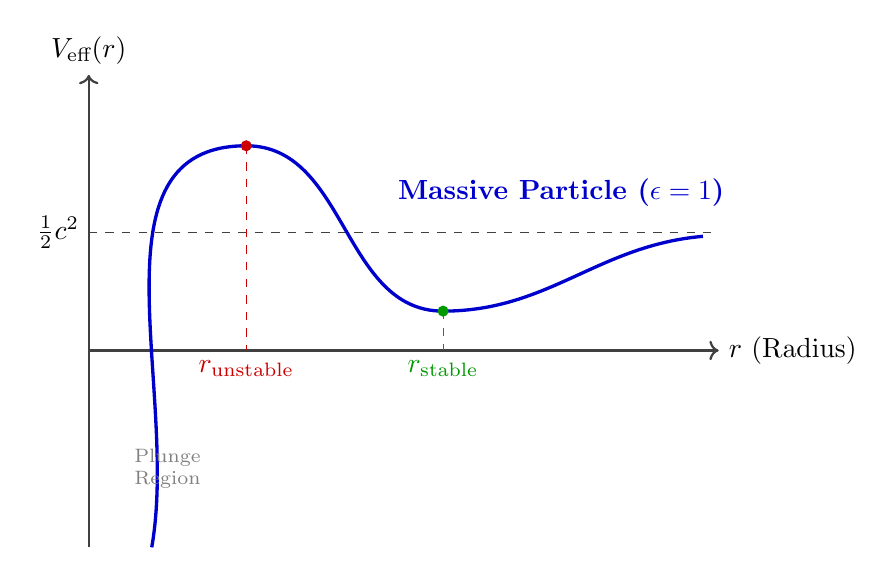
\begin{tikzpicture}[scale=1.0]
  % Axes
  \draw[->, thick, darkgray] (0,-2.5) -- (0, 3.5) node[above, text=black] {$V_{\text{eff}}(r)$};
  \draw[->, thick, darkgray] (0,0) -- (8, 0) node[right, text=black] {$r$ (Radius)};
  
  % Asymptote for massive particles (E_rest / m c^2)
  \draw[dashed, darkgray] (0, 1.5) node[left, text=black] {$\frac{1}{2}c^2$} -- (8, 1.5);

  % Extrema Coordinates
  \coordinate (Peak) at (2.0, 2.6);
  \coordinate (Min) at (4.5, 0.5);

  % The Effective Potential Curve (Massive Particle)
  \draw[very thick, blue!80!black] (0.8, -2.5)
    to[out=80, in=180] (Peak)
    to[out=0, in=180] (Min)
    to[out=0, in=185] (7.8, 1.45);
    
  % Annotations for Extrema
  \draw[dashed, red!80!black] (Peak) -- (2.0, 0) node[below] {$r_{\text{unstable}}$};
  \draw[dashed, green!60!black] (Min) -- (4.5, 0) node[below] {$r_{\text{stable}}$};
  
  \fill[red!80!black] (Peak) circle (2pt);
  \fill[green!60!black] (Min) circle (2pt);

  % Add a label for the curve
  \node[blue!80!black, font=\bfseries] at (6, 2.0) {Massive Particle ($\epsilon=1$)};
  
  % Singularity Region
  \node[align=center, font=\scriptsize, gray] at (1.0, -1.5) {Plunge \\ Region};
\end{tikzpicture}
\end{center}





For photons ($\epsilon=0$):
\begin{equation}
V_{\text{eff}}(r) = \frac{L^{2}}{2r^{2}} - \frac{GML^{2}}{r^{3}}.
\end{equation}
\begin{equation}
\frac{dV_{\text{eff}}}{dr} = -\frac{L^{2}}{r^{3}} + \frac{3GML^{2}}{r^{4}}.
\end{equation}
\begin{equation}
\frac{L^{2}}{r^{3}} = \frac{3GML^{2}}{r^{4}} \quad \implies \quad r_{c} = 3GM.
\end{equation}
\begin{equation}
\frac{d^{2}V_{\text{eff}}}{dr^{2}} = \frac{3L^{2}}{r^{4}} - \frac{12GML^{2}}{r^{5}}.
\end{equation}
\begin{equation}
\frac{d^{2}V_{\text{eff}}}{dr^{2}}\bigg|*{r=3GM} = -\frac{L^{2}}{81G^{4}M^{4}}.
\end{equation}
For massive particles ($\epsilon=1$):
\begin{equation}
V*{\text{eff}}(r) = \frac{1}{2} - \frac{GM}{r} + \frac{L^{2}}{2r^{2}} - \frac{GML^{2}}{r^{3}}.
\end{equation}
\begin{equation}
\frac{dV_{\text{eff}}}{dr} = \frac{GM}{r^{2}} - \frac{L^{2}}{r^{3}} + \frac{3GML^{2}}{r^{4}} = 0.
\end{equation}
\begin{equation}
r^{2} - \left(\frac{L^{2}}{GM}\right)r + 3L^{2} = 0.
\end{equation}
\begin{equation}
\label{eq:circular_radii}
r_{c} = \frac{L^{2} \pm \sqrt{L^{4} - 12G^{2}M^{2}L^{2}}}{2GM}.
\end{equation}
Critical threshold angular momentum for orbits:
\begin{equation}
L_{c} = \sqrt{12}GM.
\end{equation}
Innermost Stable Circular Orbit (ISCO):
\begin{equation}
r_{\text{ISCO}} = \frac{12G^{2}M^{2}}{2GM} = 6GM.
\end{equation}

\section{Experimental Tests of General Relativity}
\subsection{The Precession of Perihelia}
\begin{equation}
\label{eq:radial_energy_massive}
\frac{1}{2}\left(\frac{dr}{d\lambda}\right)^{2} + \frac{1}{2} - \frac{GM}{r} + \frac{L^{2}}{2r^{2}} - \frac{GML^{2}}{r^{3}} = \frac{1}{2}E^{2}.
\end{equation}
\begin{equation}
\frac{dr}{d\lambda} = \frac{dr}{d\phi}\frac{d\phi}{d\lambda} = \frac{L}{r^{2}}\frac{dr}{d\phi}.
\end{equation}
\begin{equation}
\frac{L^{2}}{r^{4}}\left(\frac{dr}{d\phi}\right)^{2} + 1 - \frac{2GM}{r} + \frac{L^{2}}{r^{2}} - \frac{2GML^{2}}{r^{3}} = E^{2}.
\end{equation}
Substituting $u = 1/r$:
\begin{equation}
\frac{dr}{d\phi} = -r^{2}\frac{du}{d\phi}.
\end{equation}
\begin{equation}
L^{2}\left(\frac{du}{d\phi}\right)^{2} + 1 - 2GMu + L^{2}u^{2} - 2GML^{2}u^{3} = E^{2}.
\end{equation}
\begin{equation}
2L^{2}\left(\frac{du}{d\phi}\right)\frac{d^{2}u}{d\phi^{2}} - 2GM\frac{du}{d\phi} + 2L^{2}u\frac{du}{d\phi} - 6GML^{2}u^{2}\frac{du}{d\phi} = 0.
\end{equation}
\begin{equation}
\frac{d^{2}u}{d\phi^{2}} + u = \frac{GM}{L^{2}} + 3GMu^{2}.
\end{equation}
Scaling $x = L^2 u / GM$:
\begin{equation}
x = \frac{L^{2}}{GM}u = \frac{L^{2}}{GMr}.
\end{equation}
\begin{equation}
\label{eq:perihelion_ode}
\frac{d^{2}x}{d\phi^{2}} - 1 + x = \frac{3G^{2}M^{2}}{L^{2}}x^{2}.
\end{equation}
Using perturbative expansion $x = x_0 + x_1$:
\begin{equation}
x(\phi) = x_{0}(\phi) + x_{1}(\phi).
\end{equation}
\begin{align}
\text{Zeroth order: } & \frac{d^{2}x_{0}}{d\phi^{2}} + x_{0} = 1, \label{eq:zero_order} \\
\text{First order: } & \frac{d^{2}x_{1}}{d\phi^{2}} + x_{1} = \alpha x_{0}^{2}. \label{eq:first_order}
\end{align}
\begin{equation}
\label{eq:x0_solution}
x_{0}(\phi) = 1 + e \cos\phi,
\end{equation}
\begin{equation}
\frac{d^{2}x_{1}}{d\phi^{2}} + x_{1} = \alpha (1 + e \cos\phi)^{2} = \alpha (1 + 2e \cos\phi + e^{2} \cos^{2}\phi).
\end{equation}
\begin{equation}
\frac{d^{2}x_{1}}{d\phi^{2}} + x_{1} = \alpha \left[ \left(1 + \frac{1}{2}e^{2}\right) + 2e \cos\phi + \frac{1}{2}e^{2} \cos 2\phi \right].
\end{equation}
\begin{align}
\frac{d}{d\phi}(D\phi\sin\phi) &= D\sin\phi + D\phi\cos\phi, \\
\frac{d^{2}}{d\phi^{2}}(D\phi\sin\phi) &= 2D\cos\phi - D\phi\sin\phi.
\end{align}
\begin{equation}
x_{1}(\phi) = \alpha \left[ \left(1 + \frac{1}{2}e^{2}\right) + e\phi\sin\phi - \frac{1}{6}e^{2}\cos 2\phi \right].
\end{equation}
\begin{equation}
x(\phi) \approx 1 + e\cos\phi + \alpha e \phi \sin\phi.
\end{equation}
\begin{equation}
\label{eq:precession_phase}
x(\phi) \approx 1 + e \cos(\phi - \alpha\phi) = 1 + e \cos[(1-\alpha)\phi].
\end{equation}


\begin{center}
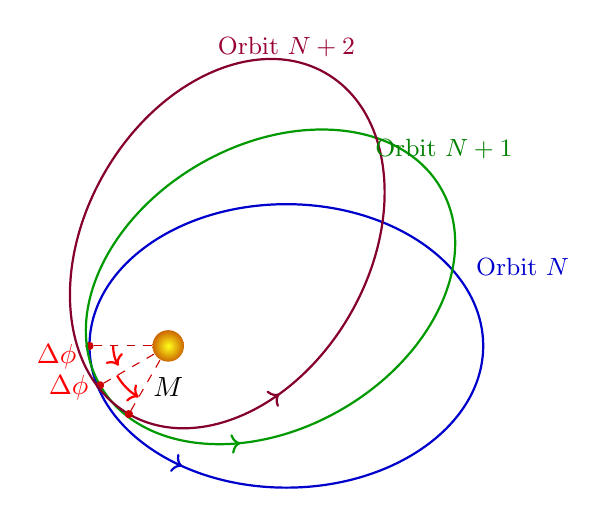
\begin{tikzpicture}[scale=1.0]
  \coordinate (O) at (0,0);

  % Orbit 1 (Initial)
  \begin{scope}[rotate=0]
    \draw[thick, blue!80!black, decoration={markings, mark=at position 0.65 with {\arrow{>}}}, postaction={decorate}] (1.5, 0) ellipse (2.5 and 1.8);
    \draw[dashed, red!80!black] (O) -- (-1, 0) coordinate (P1);
    \fill[red!80!black] (-1,0) circle (1.5pt);
  \end{scope}

  % Orbit 2 (Precessed)
  \begin{scope}[rotate=30]
    \draw[thick, green!60!black, decoration={markings, mark=at position 0.65 with {\arrow{>}}}, postaction={decorate}] (1.5, 0) ellipse (2.5 and 1.8);
    \draw[dashed, red!80!black] (O) -- (-1, 0) coordinate (P2);
    \fill[red!80!black] (-1,0) circle (1.5pt);
  \end{scope}
  
  % Orbit 3 (Further Precessed)
  \begin{scope}[rotate=60]
    \draw[thick, purple!70!black, decoration={markings, mark=at position 0.65 with {\arrow{>}}}, postaction={decorate}] (1.5, 0) ellipse (2.5 and 1.8);
    \draw[dashed, red!80!black] (O) -- (-1, 0) coordinate (P3);
    \fill[red!80!black] (-1,0) circle (1.5pt);
  \end{scope}

  % Central mass (Sun/Black Hole)
  \shade[inner color=yellow!90!white, outer color=orange!80!black] (O) circle (0.2) node[below=8pt, text=black, font=\bfseries] {$M$};

  % Precession angle arcs
  \draw[->, thick, red] (-0.7, 0) arc (180:210:0.5) node[midway, left=10pt] {$\Delta\phi$};
  \draw[->, thick, red] (-0.65, -0.375) arc (210:240:0.75) node[midway, left=10pt] {$\Delta\phi$};

  % Legend / Labels
  \node[blue!80!black, font=\small] at (4.5, 1.0) {Orbit $N$};
  \node[green!50!black, font=\small] at (3.5, 2.5) {Orbit $N+1$};
  \node[purple!80!black, font=\small] at (1.5, 3.8) {Orbit $N+2$};

\end{tikzpicture}
\end{center}

\begin{equation}
(1 - \alpha)\phi_{p} = 2\pi \quad \implies \quad \phi_{p} = \frac{2\pi}{1-\alpha}.
\end{equation}
\begin{equation}
\phi_{p} \approx 2\pi(1 + \alpha) = 2\pi + 2\pi\alpha.
\end{equation}
\begin{equation}
\Delta\phi = 2\pi\alpha = \frac{6\pi G^{2}M^{2}}{L^{2}}.
\end{equation}
\begin{equation}
\Delta\phi = \frac{6\pi GM}{c^{2}a(1-e^{2})} \text{ radians per orbit}.
\end{equation}

\subsection{Gravitational Redshift}
\begin{equation}
g_{tt}(U^{t})^{2} = -1 \quad \implies \quad -\left(1-\frac{2GM}{r}\right)(U^{t})^{2} = -1.
\end{equation}
\begin{equation}
U^{\mu} = \left( \left(1-\frac{2GM}{r}\right)^{-1/2}, 0, 0, 0 \right).
\end{equation}
\begin{equation}
\omega = -g_{\mu\nu}p^{\mu}U^{\nu}.
\end{equation}
\begin{equation}
\omega = -g_{tt} p^{t} U^{t} = -\left[ -\left(1-\frac{2GM}{r}\right) \right] \left( \frac{dt}{d\lambda} \right) \left(1-\frac{2GM}{r}\right)^{-1/2}.
\end{equation}
\begin{equation}
E = \left(1-\frac{2GM}{r}\right)\frac{dt}{d\lambda} \quad \implies \quad \frac{dt}{d\lambda} = E \left(1-\frac{2GM}{r}\right)^{-1}.
\end{equation}
\begin{align}
\omega &= \left(1-\frac{2GM}{r}\right) \left[ E \left(1-\frac{2GM}{r}\right)^{-1} \right] \left(1-\frac{2GM}{r}\right)^{-1/2} \nonumber \\
\omega &= E \left(1-\frac{2GM}{r}\right)^{-1/2}.
\end{align}
\begin{equation}
\frac{\omega_{2}}{\omega_{1}} = \frac{ E \left(1-\frac{2GM}{r_{2}}\right)^{-1/2} }{ E \left(1-\frac{2GM}{r_{1}}\right)^{-1/2} } = \left( \frac{1-\frac{2GM}{r_{1}}}{1-\frac{2GM}{r_{2}}} \right)^{1/2}.
\end{equation}
Weak field limit:
\begin{align}
\frac{\omega_{2}}{\omega_{1}} &= \left(1-\frac{2GM}{r_{1}}\right)^{1/2} \left(1-\frac{2GM}{r_{2}}\right)^{-1/2} \nonumber \\
&\approx \left(1 - \frac{GM}{r_{1}}\right) \left(1 + \frac{GM}{r_{2}}\right) \nonumber \\
&\approx 1 - \frac{GM}{r_{1}} + \frac{GM}{r_{2}} + \mathcal{O}\left(\frac{G^{2}M^{2}}{r^{2}}\right).
\end{align}
\begin{equation}
\frac{\omega_{2}}{\omega_{1}} \approx 1 + \Phi(r_{1}) - \Phi(r_{2}) = 1 - \Delta\Phi.
\end{equation}

\section{Schwarzschild Black Holes and Causal Structure}
\subsection{Causal Structure in Schwarzschild Coordinates}
\begin{equation}
0 = -\left(1-\frac{2GM}{r}\right)dt^{2} + \left(1-\frac{2GM}{r}\right)^{-1}dr^{2}.
\end{equation}
\begin{equation}
\label{eq:radial_light_cone}
\frac{dt}{dr} = \pm \left( 1 - \frac{2GM}{r} \right)^{-1},
\end{equation}
\begin{equation}
\lim_{r \to 2GM} \frac{dt}{dr} = \pm \infty.
\end{equation}


\begin{center}
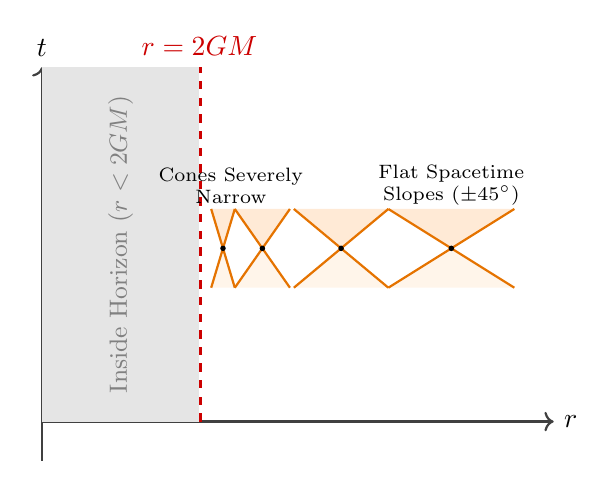
\begin{tikzpicture}[scale=1.0]
  % Axes
  \draw[->, thick, darkgray] (0,-0.5) -- (0, 4.5) node[above, text=black] {$t$};
  \draw[->, thick, darkgray] (0,0) -- (6.5, 0) node[right, text=black] {$r$};

  % Horizon line
  \draw[ultra thick, dashed, red!80!black] (2.0, 0) -- (2.0, 4.5) node[above] {$r = 2GM$};
  
  % Singularity placeholder shaded area
  \fill[gray!20] (0,0) rectangle (2.0, 4.5);
  \node[rotate=90, gray, font=\small] at (1.0, 2.25) {Inside Horizon ($r < 2GM$)};

  % Light cones macro
  \newcommand{\schwarzschildcone}[3]{
    % #1: center x, #2: center y, #3: width (dt/dr slope factor)
    \begin{scope}[shift={(#1,#2)}]
      \fill[orange!20, opacity=0.8] (0,0) -- (-#3, 0.5) -- (#3, 0.5) -- cycle;
      \fill[orange!10, opacity=0.8] (0,0) -- (-#3, -0.5) -- (#3, -0.5) -- cycle;
      \draw[thick, orange!90!black] (-#3, -0.5) -- (#3, 0.5);
      \draw[thick, orange!90!black] (#3, -0.5) -- (-#3, 0.5);
      \fill[black] (0,0) circle (1pt);
    \end{scope}
  }

  % Draw light cones at different radii
  % As r -> 2GM, dt/dr -> infinity, so the cone becomes extremely narrow in space (x-width decreases)
  \schwarzschildcone{2.3}{2.2}{0.15}
  \schwarzschildcone{2.8}{2.2}{0.35}
  \schwarzschildcone{3.8}{2.2}{0.6}
  \schwarzschildcone{5.2}{2.2}{0.8}

  % Labels
  \node[font=\scriptsize, align=center] at (5.2, 3.0) {Flat Spacetime \\ Slopes ($\pm 45^\circ$)};
  \node[font=\scriptsize, align=center] at (2.4, 3.0) {Cones Severely \\ Narrow};

\end{tikzpicture}
\end{center}




\subsection{The Tortoise Coordinate}
\begin{equation}
dt = \pm \frac{dr}{1 - 2GM/r} \quad \implies \quad \int dt = \pm \int \frac{r}{r - 2GM} dr.
\end{equation}
\begin{equation}
\pm t = r + 2GM \ln\left| \frac{r}{2GM} - 1 \right| + \text{constant}.
\end{equation}
\begin{equation}
\label{eq:tortoise_def}
r^{*} \equiv r + 2GM \ln\left| \frac{r}{2GM} - 1 \right|.
\end{equation}
\begin{equation}
dr^{*} = \left( 1 + \frac{2GM}{r - 2GM} \right) dr = \left( \frac{r}{r - 2GM} \right) dr = \left( 1 - \frac{2GM}{r} \right)^{-1} dr.
\end{equation}
\begin{equation}
\left( 1 - \frac{2GM}{r} \right)^{-1} dr^{2} = \left( 1 - \frac{2GM}{r} \right) (dr^{*})^{2}.
\end{equation}
\begin{equation}
ds^{2} = \left( 1 - \frac{2GM}{r} \right) \left[ -dt^{2} + (dr^{*})^{2} \right] + r^{2} d\Omega^{2},
\end{equation}

\subsection{Eddington-Finkelstein Coordinates}
\begin{equation}
\label{eq:advanced_v}
v \equiv t + r^{*}.
\end{equation}
\begin{equation}
dt = dv - dr^{*} = dv - \left( 1 - \frac{2GM}{r} \right)^{-1} dr.
\end{equation}
\begin{align}
ds^{2} &= -\left( 1 - \frac{2GM}{r} \right) \left[ dv - \left( 1 - \frac{2GM}{r} \right)^{-1} dr \right]^{2} + \left( 1 - \frac{2GM}{r} \right)^{-1} dr^{2} + r^{2} d\Omega^{2} \nonumber \\
&= -\left( 1 - \frac{2GM}{r} \right) \left[ dv^{2} - 2\left( 1 - \frac{2GM}{r} \right)^{-1} dv dr + \left( 1 - \frac{2GM}{r} \right)^{-2} dr^{2} \right] \nonumber \\
&\quad + \left( 1 - \frac{2GM}{r} \right)^{-1} dr^{2} + r^{2} d\Omega^{2}.
\end{align}
\begin{align}
ds^{2} &= -\left( 1 - \frac{2GM}{r} \right)dv^{2} + 2 dv dr - \left( 1 - \frac{2GM}{r} \right)^{-1} dr^{2} + \left( 1 - \frac{2GM}{r} \right)^{-1} dr^{2} + r^{2} d\Omega^{2}.
\end{align}
\begin{equation}
\label{eq:eddington_metric}
ds^{2} = -\left( 1 - \frac{2GM}{r} \right)dv^{2} + 2 dv dr + r^{2} d\Omega^{2}.
\end{equation}
\begin{equation}
g_{\mu\nu} =
\begin{pmatrix}
-\left(1-\frac{2GM}{r}\right) & 1 & 0 & 0 \\
1 & 0 & 0 & 0 \\
0 & 0 & r^{2} & 0 \\
0 & 0 & 0 & r^{2}\sin^{2}\theta
\end{pmatrix}
\end{equation}
\begin{equation}
g = \det(g_{\mu\nu}) = (-(0) - (1)(1))(r^{2})(r^{2}\sin^{2}\theta) = -r^{4}\sin^{2}\theta.
\end{equation}

\subsection{The Event Horizon and the Tipping of Light Cones}
\begin{equation}
0 = -\left( 1 - \frac{2GM}{r} \right)dv^{2} + 2 dv dr = dv \left[ -\left( 1 - \frac{2GM}{r} \right)dv + 2dr \right].
\end{equation}
\begin{align}
\text{Ingoing null geodesics: } \quad &\frac{dv}{dr} = 0 \quad \implies \quad v = \text{constant}, \\
\text{Outgoing null geodesics: } \quad &\frac{dv}{dr} = 2 \left( 1 - \frac{2GM}{r} \right)^{-1}.
\end{align}


\begin{center}
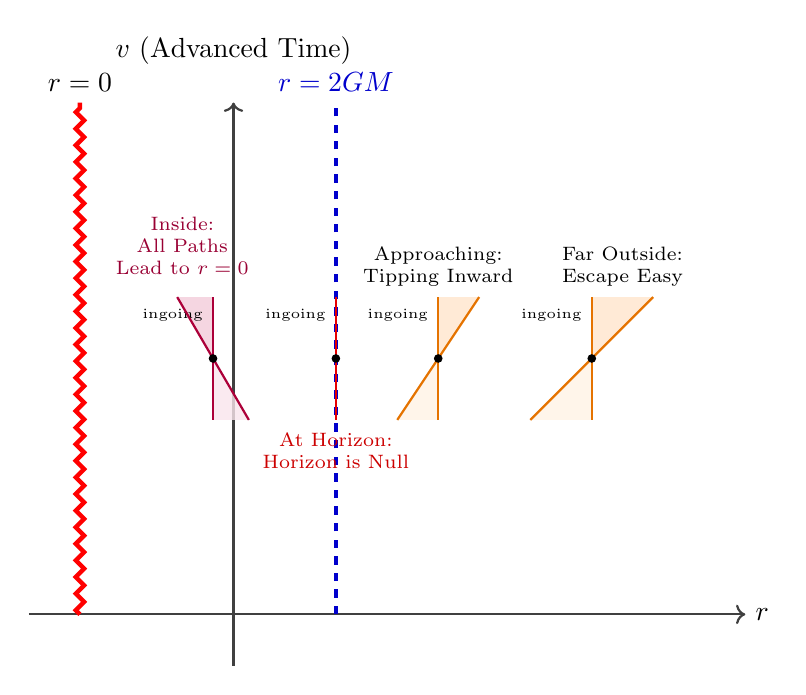
\begin{tikzpicture}[scale=1.3]
  % Axes
  \draw[->, thick, darkgray] (2.0,-0.5) -- (2.0, 5) node[above=10pt, text=black] {$v$ (Advanced Time)};
  \draw[->, thick, darkgray] (0,0) -- (7, 0) node[right, text=black] {$r$};

  % Singularity at r=0
  \draw[ultra thick, decorate, decoration={zigzag, segment length=6pt, amplitude=1.5pt}, red] 
    (0.5, 0) -- (0.5, 5) node[above, text=black] {$r = 0$};

  % Event Horizon
  \draw[ultra thick, dashed, blue!80!black] (3.0, 0) -- (3.0, 5) node[above] {$r = 2GM$};

  % Light Cones Macro for EF Coordinates
  % Ingoing line is always v = const (vertical on this grid).
  % Outgoing line has slope dv/dr = 2 / (1 - 2GM/r).
  \newcommand{\efcone}[4]{
    % #1: center x, #2: center y, #3: right bound slope displacement, #4: color choice
    \begin{scope}[shift={(#1,#2)}]
      \fill[#4!20, opacity=0.8] (0,0) -- (0, 0.6) -- (#3, 0.6) -- cycle;
      \fill[#4!10, opacity=0.8] (0,0) -- (0, -0.6) -- (-#3, -0.6) -- cycle;
      \draw[thick, #4!90!black] (0, -0.6) -- (0, 0.6) node[pos=0.85, left, font=\tiny, text=black] {ingoing};
      \draw[thick, #4!90!black] (-#3, -0.6) -- (#3, 0.6);
      \fill[black] (0,0) circle (1.2pt);
    \end{scope}
  }

  % Outside Horizon: Outgoing boundary points right (away from horizon)
  \efcone{5.5}{2.5}{0.6}{orange}
  \node[font=\scriptsize, align=center] at (5.8, 3.4) {Far Outside:\\Escape Easy};

  \efcone{4.0}{2.5}{0.4}{orange}
  \node[font=\scriptsize, align=center] at (4.0, 3.4) {Approaching:\\Tipping Inward};

  % At Horizon: Outgoing boundary becomes completely vertical (dv/dr -> infinity)
  \efcone{3.0}{2.5}{0.0}{red}
  \node[red!80!black, font=\scriptsize, align=center] at (3.0, 1.6) {At Horizon:\\Horizon is Null};

  % Inside Horizon: Outgoing boundary tilts left (towards singularity)
  \efcone{1.8}{2.5}{-0.35}{purple}
  \node[purple!80!black, font=\scriptsize, align=center] at (1.5, 3.6) {Inside:\\All Paths\\Lead to $r=0$};

\end{tikzpicture}
\end{center}

The surface $r=2GM$ forms an event horizon because all future light cones are tilted inward, making escape impossible.

\begin{equation}
\frac{1}{2} m v_{\text{esc}}^{2} = \frac{GMm}{r} \quad \implies \quad v_{\text{esc}} = \sqrt{\frac{2GM}{r}}.
\end{equation}

\end{document}